%---------------------------------------------------------------------------%
%-                                                                         -%
%-                           LaTeX Template                                -%
%-                                                                         -%
%---------------------------------------------------------------------------%
%- Copyright (C) Huangrui Mo <huangrui.mo@gmail.com> 
%- This is free software: you can redistribute it and/or modify it
%- under the terms of the GNU General Public License as published by
%- the Free Software Foundation, either version 3 of the License, or
%- (at your option) any later version.
%---------------------------------------------------------------------------%
%->> Document class declaration
%---------------------------------------------------------------------------%
\documentclass[twoside]{Style/ucasthesis}%
%- Multiple optional arguments:
%- [<oneside|twoside|print>]% oneside eprint, twoside eprint, or paper print
%- [fontset=<adobe|...>]% specify font set to replace automatic detection
%- [scheme=plain]% thesis writing of international students
%- [draftversion]% show draft version information
%- [standard options for ctex book class: draft|paper size|font size|...]%
%---------------------------------------------------------------------------%
%->> Document settings
%---------------------------------------------------------------------------%
\usepackage[authoryear,list]{Style/artratex}% document settings
%- usage: \usepackage[option1,option2,...,optionN]{artratex}
%- Multiple optional arguments:
%- [bibtex|biber]% set bibliography processor and package
%- [<numbers|super|authoryear|alpha>]% set citation and reference style
%- <numbers>: textual: Jones [1]; parenthetical: [1]
%- <super>: textual: Jones superscript [1]; parenthetical: superscript [1]
%- <authoryear>: textual: Jones (1995); parenthetical: (Jones, 1995)
%- <alpha>: textual: not available; parenthetical: [Jon95]
%- [geometry]% reconfigure page layout via geometry package
%- [lscape]% provide landscape layout environment
%- [xhf]% disable header and footer via fancyhdr package
%- [color]% provide color support via xcolor package
%- [background]% enable page background
%- [tikz]% provide complex diagrams via tikz package
%- [table]% provide complex tables via ctable package
%- [list]% provide enhanced list environments for algorithm and coding
%- [math]% enable some extra math packages
%- [xlink]% disable link colors
\usepackage{Style/artracom}% user defined commands

%---------------------------------------------------------------------------%
%->> Document inclusion
%---------------------------------------------------------------------------%
%\includeonly{Tex/Chap_1,...,Tex/Chap_N}% selected files compilation
%---------------------------------------------------------------------------%
%->> Document content
%---------------------------------------------------------------------------%
%-
%-> Titlepage information
%-
\usepackage{booktabs}
\usepackage{multirow}
%---------------------------------------------------------------------------%
%->> Titlepage information
%---------------------------------------------------------------------------%
%-
%-> 中文封面信息
%-
\confidential{}% 密级:只有涉密论文才填写
\schoollogo[scale=0.095]{ucas_logo}% 校徽
\title{面向加密流量的主机属性发现}% 论文中文题目
\author{范鑫磊}% 论文作者
\advisor{周晓飞~副研究员\\中国科学院信息工程研究所}% 指导教师:姓名 专业技术职务 工作单位
%\advisor{指导教师一\\指导教师二\\指导教师三}% 多行指导教师示例
\degree{硕士}% 学位:学士、硕士、博士
\degreetype{工学}% 学位类别:理学、工学、工程、医学等
\major{网络空间安全}% 二级学科专业名称
\institute{中国科学院信息工程研究所}% 院系名称
%\institute{中国科学院力学研究所\\流固耦合实验室}% 多行院系名称示例
\date{2020~年~6~月}% 毕业日期:夏季为6月、冬季为12月
%-
%-> 英文封面信息
%-
\TITLE{Host Attribute Discovery for Encrypted Traffic}% 论文英文题目
\AUTHOR{Fan Xinlei}% 论文作者
\ADVISOR{Supervisor: Professor Zhou Xiaofei}% 指导教师
\DEGREE{Master}% 学位:Bachelor, Master, Doctor, Postdoctor。封面据英文学位名称自动切换,需确保拼写准确
\DEGREETYPE{Science in Engineering}% 学位类别:Philosophy, Natural Science, Engineering, Economics, Agriculture 等
\MAJOR{Cyberspace security}% 二级学科专业名称
\INSTITUTE{Institute of Information Engineering, Chinese Academy of Sciences}% 院系名称
\DATE{June, 2020}% 毕业日期:夏季为June、冬季为December
%---------------------------------------------------------------------------%
%
\begin{document}
%-
%-> Frontmatter: title page, abstract, content list, symbol list, preface
%-
\frontmatter% initialize the environment
%---------------------------------------------------------------------------%
%->> Frontmatter
%---------------------------------------------------------------------------%
%-
%-> 生成封面
%-
\maketitle% 生成中文封面
\MAKETITLE% 生成英文封面
%-
%-> 作者声明
%-
\makedeclaration% 生成声明页
%-
%-> 中文摘要
%-
\intobmk\chapter*{摘\quad 要}% 显示在书签但不显示在目录
\setcounter{page}{1}% 开始页码
\pagenumbering{Roman}% 页码符号

随着互联网规模的快速增长,网络安全问题得到越来越多的重视。无论是信息时代中的国家安全,电子商务应用中的财产安全,还是即时通信应用中的隐私安全,都需要网络安全技术的保障。而在网络攻防领域中,对主机信息的采集既是网络攻击的首要任务,又是入侵防御的关键所在。一方面,攻击者需要基于目标主机信息确定下一步入侵手段,另一方面,网络管理员可以利用本地网络中的主机信息优化防御策略,及时修补漏洞。

与此同时,加密协议和伪装技术的普及,虽然从多个方面保护了企业和个人的数据安全,但也给主机属性识别技术带来了新的挑战。因此,本文针对加密网络中的被动主机属性发现技术进行深入研究,从流量数据中提取人工特征和原始载荷特征,结合LightGBM模型、神经网络模型、Stacking集成技术等算法构建分类器,并设计和开发一套原型系统,用于识别真实网络中海量主机的操作系统类型、版本以及浏览器类型等属性信息。

本文的主要贡献包括:
\begin{enumerate}
\item
开放环境中的细粒度主机属性发现。本文以双向流为单位,从TLS会话中提取13维协议首部字段特征和3类流统计特征,协议首部包括IP协议首部、TCP协议首部以及TLS协议首部等,流统计特征包括包长序列统计特征、时间序列统计特征以及速率统计特征等。然后结合以LightGBM模型为代表的机器学习算法,实现了对开放环境中细粒度主机属性的高精度识别。
\item
基于加密流原始载荷的主机属性发现。由于人工提取特征方法的有效性过于依赖专家知识,本文提出了基于表示学习和原始字节特征的主机属性发现技术。通过提取TLS会话中TCP SYN包和TLS Client Hello包的原始字节信息,并结合以卷积神经网络模型和长短期记忆网络模型为代表的深度学习算法,可以在不需要先验知识的前提下,进一步提高开放环境中主机属性的识别精度。
\item
主机属性识别系统的设计与实现。本文利用Stacking技术,将基于人工特征的机器学习模型和基于原始字节特征的神经网络模型进行融合,开发了一套用于海量主机属性发现的原型系统。其中,流量采集模块用于在高速网络中识别并采集目标流量。特征提取模块用于从原始TLS流量中提取所需的人工特征和原始载荷特征。属性识别模块基于Stacking技术,综合分析各学习模型的检测结果,得到最终的识别信息。分类器更新模块基于对标注数据集的再学习,可以对属性识别模块中的分类器进行更新和优化。数据存储与可视化模块用于识别结果的存储和可视化展示。
\end{enumerate}

\keywords{加密流量,属性识别,机器学习}% 中文关键词
%-
%-> 英文摘要
%-
\intobmk\chapter*{Abstract}% 显示在书签但不显示在目录

With the rapid growth of the Internet, more and more attention has been paid to network security issues. Whether it is national security in the information age, property security in e-commerce applications, or privacy security in instant messaging applications, network security technology is required. In the field of network attack and defense, the collection of host information is both the primary task of network attacks and the key to intrusion prevention.On the one hand, the attacker needs to determine the next intrusion method based on the target host information. On the other hand, the network administrator can use the host information in the local network to optimize the defense strategy and patch the vulnerabilities in time.

At the same time, the popularity of encryption protocols and camouflage technology has protected the data security of enterprises and individuals from multiple aspects, but it has also brought new challenges to the identification of host attributes. Therefore, this thesis conducts in-depth research on passive host attribute discovery technology in encrypted networks, extracts artificial features and original payload features from traffic data, combines LightGBM model, neural network model, stacking ensemble technology and other algorithms to build a classifier, and designs a set of The prototype system is used to identify attribute information such as the operating system type, version, and browser type of the host in a large-scale network.

The main contributions of this thesis include:
\begin{enumerate}
\item

Fine-grained host attribute discovery in an open environment. This thesis uses two-way flow as the unit to extract the 13-dimensional protocol header field features and 3 types of flow statistical features from the TLS session. The protocol header includes IP protocol header, TCP protocol header and TLS protocol header. Flow statistical features include packet length sequence statistical features, time sequence statistical features and rate statistical features. Then combined with the machine learning algorithm represented by the LightGBM model, it realizes high-precision identification of fine-grained host attributes in an open environment.
\item

Discovery of host attributes based on the original payload of the encrypted stream. Because the effectiveness of the artificial feature extraction method depends too much on expert knowledge, this thesis proposes a host attribute discovery technique based on representation learning and original byte data. By extracting the original byte information of the TCP SYN packet and TLS Client Hello packet in the TLS session, and combining the deep learning algorithm represented by the convolutional neural network model and the long short-term memory network model, it can further improve the identification accuracy of host attributes in an open environment without requiring prior knowledge.

\item
Design and implementation of host attribute identification system. This thesis uses stacking technology to integrate machine learning model based on artificial features and neural network model based on original byte features, and develops a prototype system for mass host attribute discovery. Among them, the traffic collection module is used to identify and collect target traffic in a high-speed network. The feature extraction module is used to extract the required artificial features and original load features from the original TLS traffic. The attribute identification module is based on the stacking technology and integrates the detection results of each learning model to obtain the final identification information. The classifier update module can update and optimize the classifier in the attribute identification module by re-learning the labeled data set. The data storage and visualization module is used to store and visualize the identification results.
\end{enumerate}

\KEYWORDS{Encrypted Traffic, Attribute Identification, Machine Learning}% 英文关键词
%---------------------------------------------------------------------------%
% title page, abstract
{% content list region
\linespread{1.2}% local line space
\intobmk*{\cleardoublepage}{\contentsname}% add link to bookmark
\tableofcontents% content catalog
\intobmk*{\cleardoublepage}{\listfigurename}% add link to bookmark
\listoffigures% figure catalog
\intobmk*{\cleardoublepage}{\listtablename}% add link to bookmark
\listoftables% table catalog
}
%\intobmk\chapter*{符号列表}% 显示在书签但不显示在目录

\section*{字符}
\nomenclatureitem[\textbf{Unit}]{\textbf{Symbol}}{\textbf{Description}}
\nomenclatureitem[$\Unit{m^{2} \cdot s^{-2} \cdot K^{-1}}$]{$R$}{the gas constant}
\nomenclatureitem[$\Unit{m^{2} \cdot s^{-2} \cdot K^{-1}}$]{$C_v$}{specific heat capacity at constant volume}
\nomenclatureitem[$\Unit{m^{2} \cdot s^{-2} \cdot K^{-1}}$]{$C_p$}{specific heat capacity at constant pressure}
\nomenclatureitem[$\Unit{m^{2} \cdot s^{-2}}$]{$E$}{specific total energy}
\nomenclatureitem[$\Unit{m^{2} \cdot s^{-2}}$]{$e$}{specific internal energy}
\nomenclatureitem[$\Unit{m^{2} \cdot s^{-2}}$]{$h_T$}{specific total enthalpy}
\nomenclatureitem[$\Unit{m^{2} \cdot s^{-2}}$]{$h$}{specific enthalpy}
\nomenclatureitem[$\Unit{kg \cdot m \cdot s^{-3} \cdot K^{-1}}$]{$k$}{thermal conductivity}
\nomenclatureitem[$\Unit{kg \cdot m^{-1} \cdot s^{-2}}$]{$S_{ij}$}{deviatoric stress tensor}
\nomenclatureitem[$\Unit{kg \cdot m^{-1} \cdot s^{-2}}$]{$\tau_{ij}$}{viscous stress tensor}
\nomenclatureitem[$\Unit{1}$]{$\delta_{ij}$}{Kronecker tensor}
\nomenclatureitem[$\Unit{1}$]{$I_{ij}$}{identity tensor}

\section*{算子}
\nomenclatureitem{\textbf{Symbol}}{\textbf{Description}}
\nomenclatureitem{$\Delta$}{difference}
\nomenclatureitem{$\nabla$}{gradient operator}
\nomenclatureitem{$\delta^{\pm}$}{upwind-biased interpolation scheme}

\section*{缩写}
\nomenclatureitem{CFD}{Computational Fluid Dynamics}
\nomenclatureitem{CFL}{Courant-Friedrichs-Lewy}
\nomenclatureitem{EOS}{Equation of State}
\nomenclatureitem{JWL}{Jones-Wilkins-Lee}
\nomenclatureitem{WENO}{Weighted Essentially Non-oscillatory}
\nomenclatureitem{ZND}{Zel'dovich-von Neumann-Doering}

% symbol list, preface content
%-
%-> Mainmatter
%-
\mainmatter% initialize the environment
%---------------------------------------------------------------------------%
%->> Main content
%---------------------------------------------------------------------------%
\chapter{引言}\label{chap:introduction}
\section{研究背景}
进入21世纪以来,网络与信息技术的发展日新月异,快速改变着人们的工作和生活方式。越来越多的政府、企业建立了依赖于网络的业务信息系统,例如电子商务、网上银行、电子政务等,对社会的各行各业造成了深远的影响。

与此同时,网络安全的重要性也在不断提升。无论是即时通信技术中的隐私保护,还是网上银行和电子商务中的财产安全,乃至信息时代中的国家安全,都离不开网络安全技术的保障。根据\cite{xintong2019zhong}发布的《中国网络安全产业白皮书》统计,2018年全球网络安全产业规模达到1119.88亿美元,预计2019年增长至1216.68亿美元。从增速上看,2018年全球网络安全产业增速为11.3\%,创下自2016年以来的新高。2014-2019年全球网络安全产业规模及增速如图1.1所示。
\begin{figure}[!htbp]
    \centering
    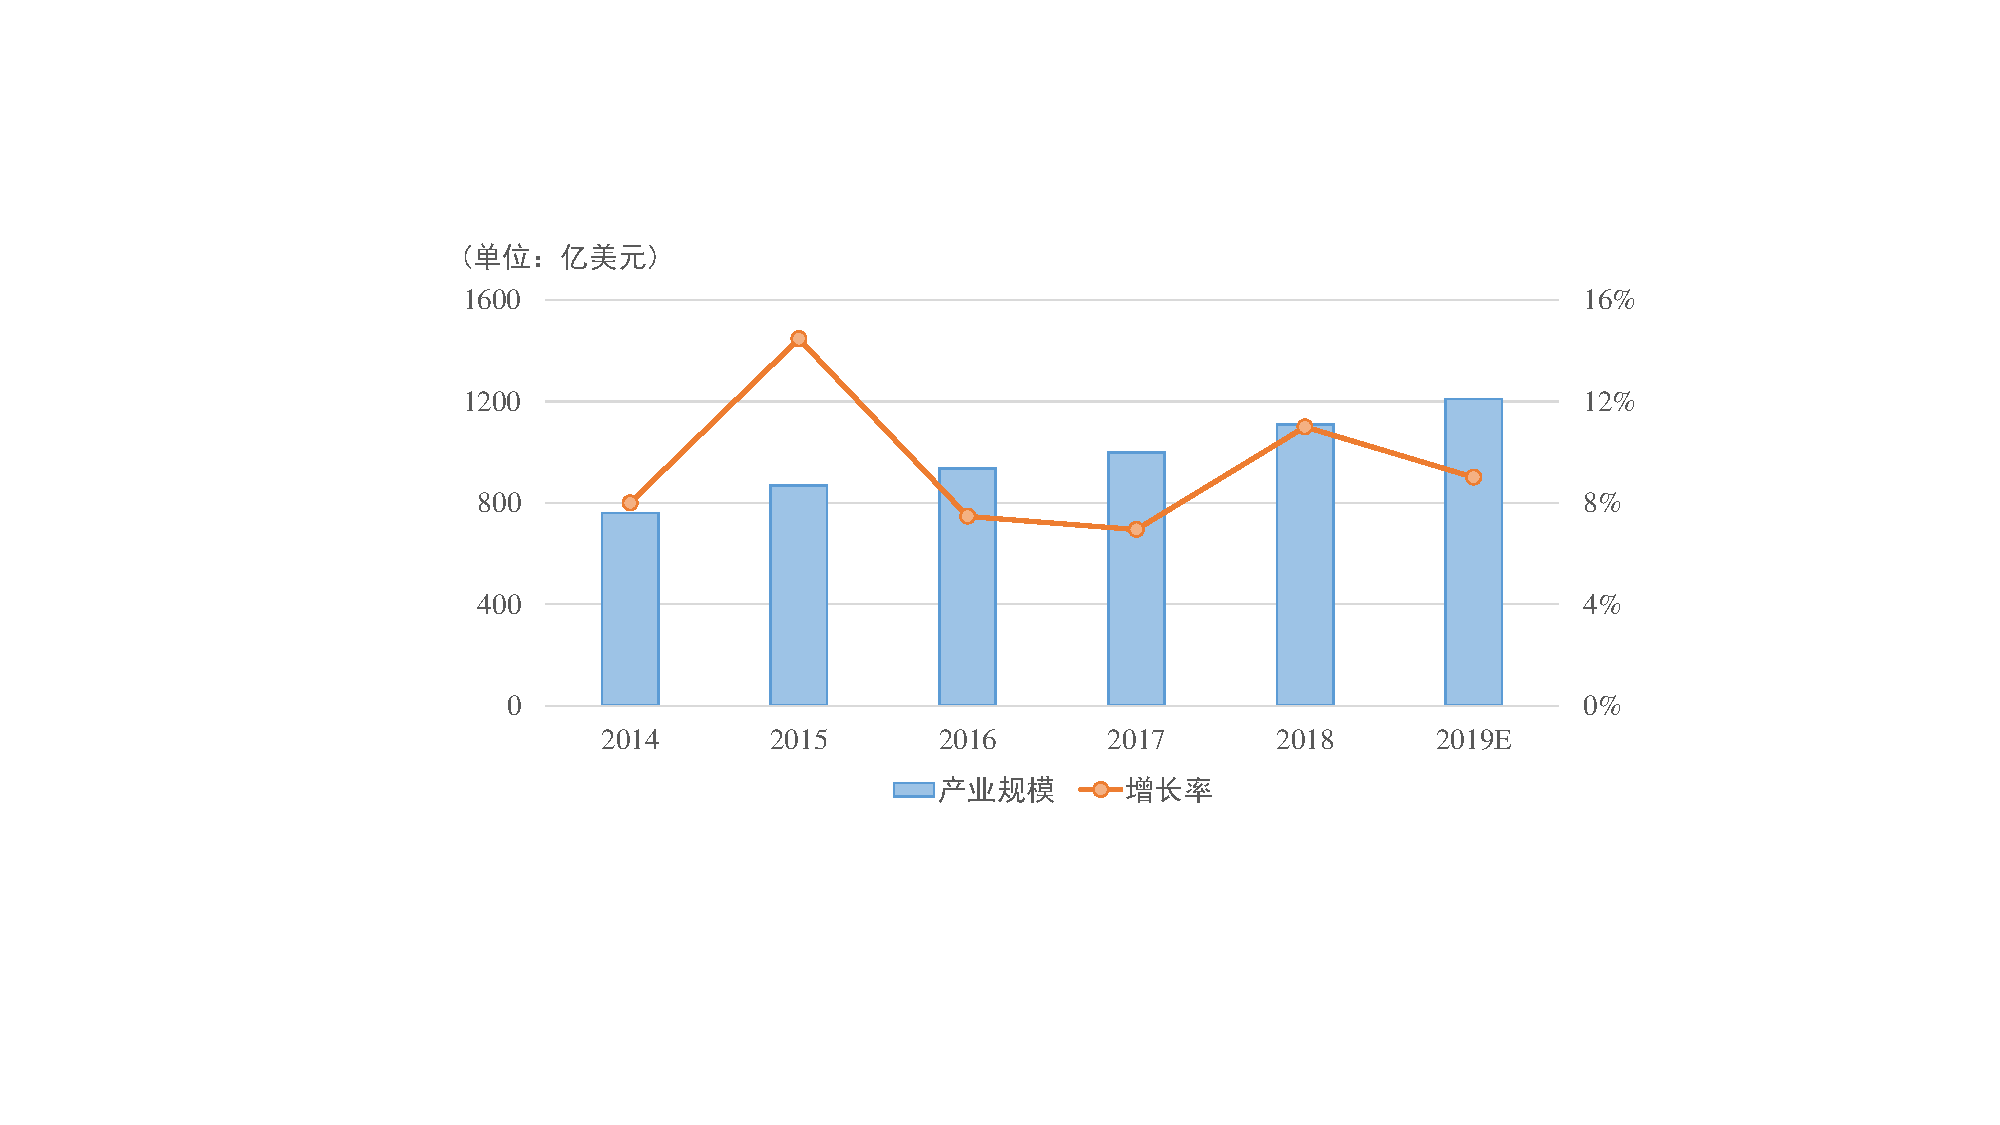
\includegraphics[width=0.9\textwidth]{网络安全产业规模及增速}
    \bicaption{2014-2019年全球网络安全产业规模及增速}{Global cyber security industry scale and growth rate, 2014-2019}
\end{figure}

此外,随着近些年互联网中移动和物联网设备数量的增多,许多企业和组织采用了日益复杂的多云架构,使得网络中的数据流不再处于传统意义上静态和高度安全的网段。同时,基于Web和移动应用的网络流量在互联网流量中的占比开始超过桌面端流量,其中大部分移动流量涉及个人敏感数据,例如支付凭证、隐私信息、社交网络等。为了适应这种变化,企业越来越依赖于利用加密手段保护数据安全,包括安全套接层(SSL)协议和传输层安全(TLS)协议。据《Google透明度报告》显示,Google产品和服务中加密流量所占比例正在平稳增长,从2014年约占48\%发展到2019年约占94\%。

\begin{figure}[!htbp]
    \centering
    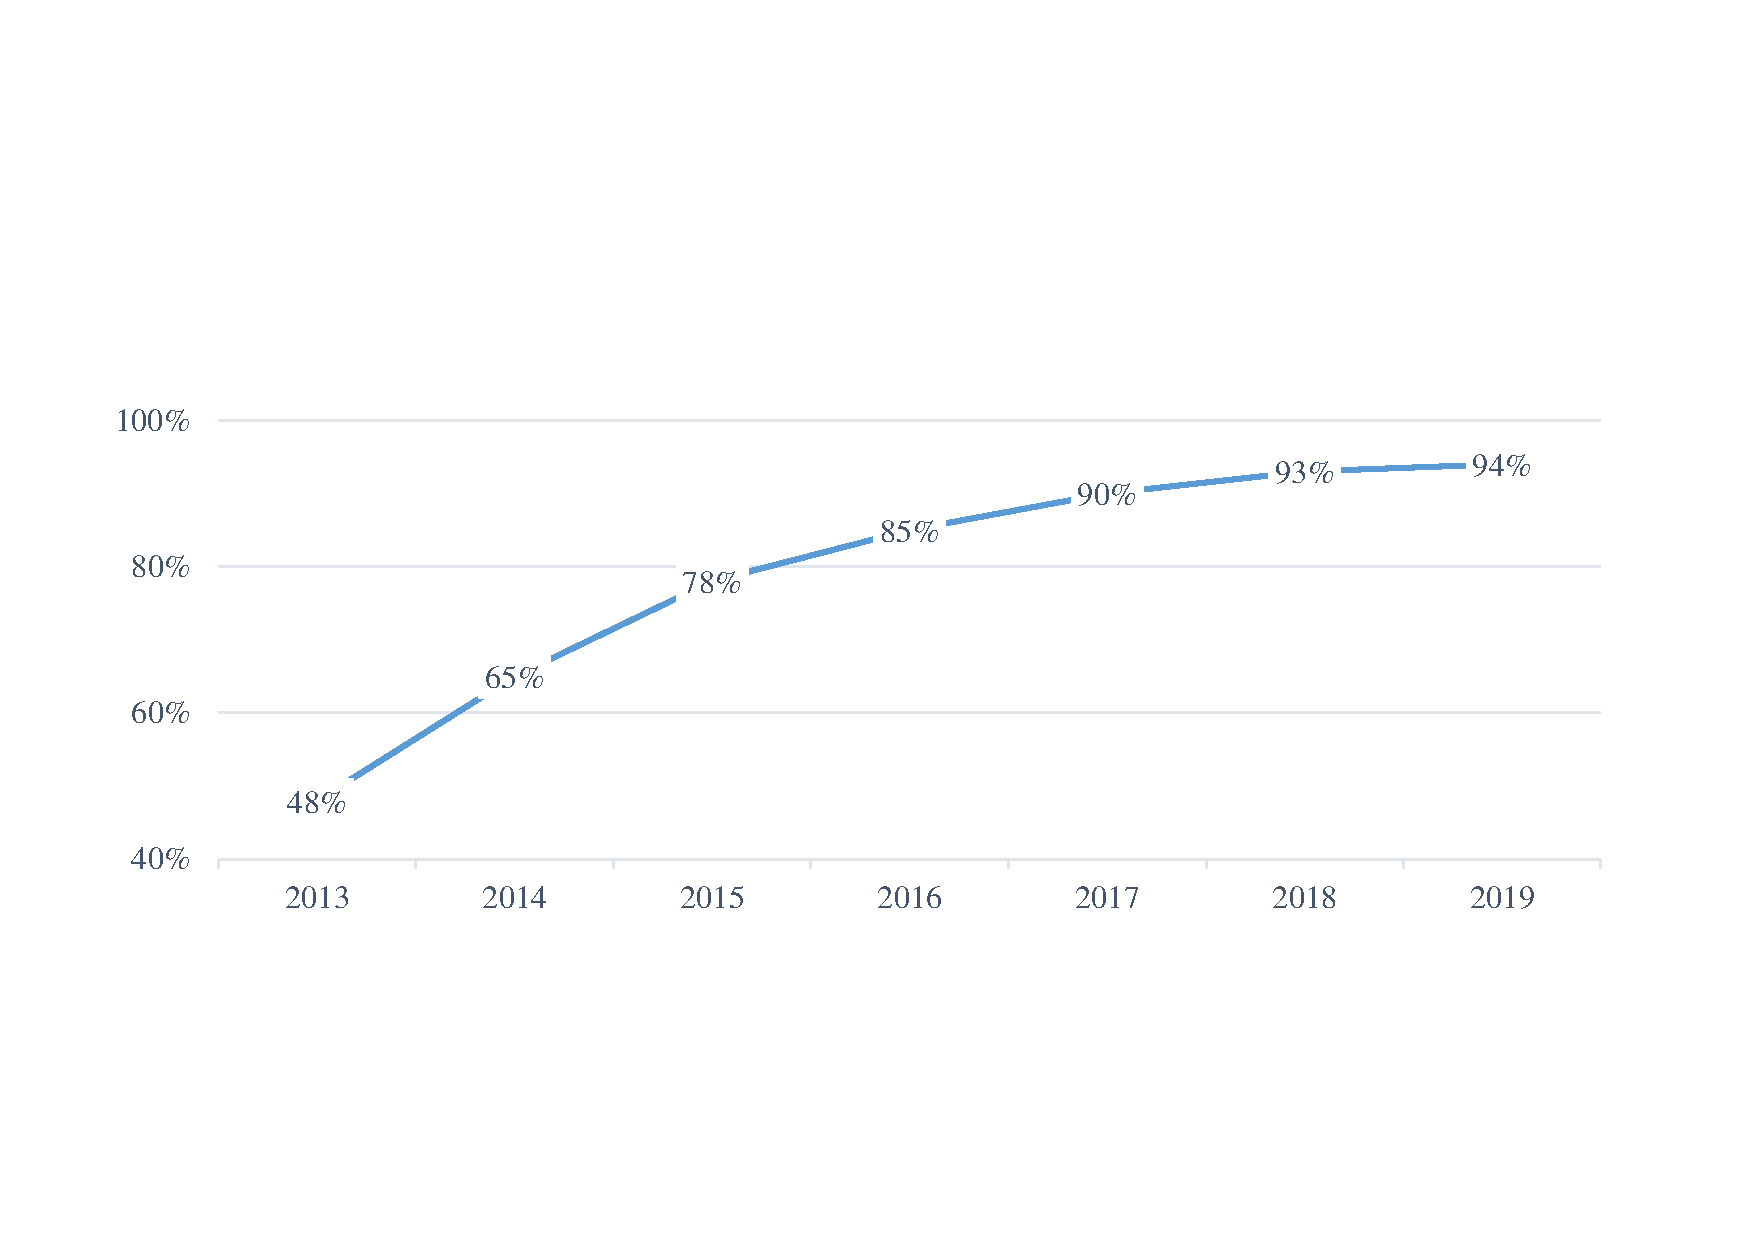
\includegraphics[width=0.9\textwidth]{1-2}
    \bicaption{2014-2019年Google产品和服务中加密流量占比增长趋势}{The growth trend of encrypted traffic in Google products and services, 2014-2019}
\end{figure}

尽管从许多方面来看,加密技术的普及对网络安全都是有利的,但同时加密流量比例的增长也对网络监管和威胁检测带来了严峻的挑战。由于加密技术只是一种工具,网络犯罪分子同样可以利用加密技术对其发起的恶意攻击进行伪装掩饰,从而逃避检测。因此,面向加密网络的流量检测技术是未来发展的必然趋势之一。

\section{研究目的和意义}

随着网络攻击行为日趋复杂,政府、企业以及个人所面临的安全威胁正在飞速增长,如蠕虫病毒、木马后门、僵尸网络、DDOS攻击等,给企业的信息网络造成严重破坏。其中,多数网络攻击的发起都与操作系统和浏览器软件漏洞有关,属于主机属性研究对象的一部分。根据\cite{guo2018zhong}发布的《中国互联网网络安全报告》显示,国家信息安全漏洞共享平台(China National Vulnerability Database, CNVD)在2018年共收录通用软硬件漏洞14201个。根据影响对象的类型,漏洞可分为:应用程序漏洞,Web应用漏洞,操作系统漏洞,网络设备漏洞,安全产品漏洞和数据库漏洞。如图1.3所示,在2018年CNVD收录的漏洞信息中,操作系统漏洞占10.6\%,Web应用漏洞占18.7\%。
\begin{figure}[!htbp]
    \centering
    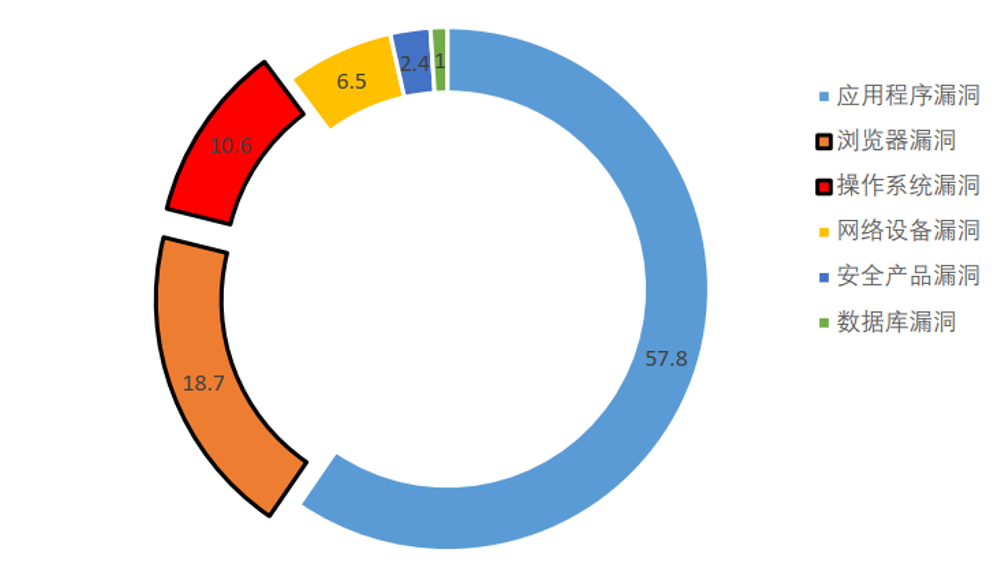
\includegraphics[width=0.8\textwidth]{1-3}
    \bicaption{2018年CNVD收录的漏洞类型分布}{Distribution of vulnerability types included in CNVD in 2018}
\end{figure}

北京时间2017年5月12日,多家安全机构监测到黑客利用美国国家安全局黑客武器库泄漏的“永恒之蓝”工具发起的网络攻击事件:大量服务器和个人电脑感染病毒后被远程控制,成为不法分子的比特币挖矿机(挖矿会耗费大量计算资源,导致机器性能降低),甚至被安装勒索软件,磁盘文件会被病毒加密为.onion或者.WNCRY后缀,用户只有支付高额赎金后才能解密恢复文件,对个人及企业的重要文件数据造成严重损失。“永恒之蓝”工具利用的是微软Windows操作系统的SMBv1协议漏洞。未经身份验证的攻击者可以向目标机器发送特制报文触发缓冲区溢出,进而在目标机器上远程执行任意代码。“永恒之蓝”工具会扫描开放445文件共享端口的Windows机器,只要用户开机上网,黑客就可能在电脑和服务器中植入勒索软件。这次攻击袭击了上百个国家不计其数的电子设备,对全球经济发展造成了难以估量的损失。

在一次完整的入侵活动中,攻击者往往采取以下几个典型步骤:信息侦察、初步入侵、系统控制、横向移动以及数据泄露等。在信息侦察阶段中,攻击者为了确定潜在目标是否满足实施入侵的条件,会利用各种技术手段对目标设备进行扫描,获取操作系统、开放端口、应用服务等信息以寻找潜在漏洞。与此相对,网络防御者可以采取安装入侵检测系统、关闭不必要的端口、提高关键设备的访问权限等手段防止攻击者获取有效信息。此外,通过研究分析攻击者侦察信息的手段,可以针对性的伪装本地主机信息,如可以通过混淆操作系统指纹使得攻击者侦察到错误信息,进而防止恶意入侵。由此可见,无论是在网络攻击还是入侵防御中,对信息的采集和识别都至关重要。一方面,攻击者需要通过目标主机信息确定下一步入侵手段,另一方面,网络管理员可以利用本地网络主机信息优化防御策略,及时修补漏洞。

综上所述,网络信息安全问题在我国以及全球日趋严重,为了国家和人民的利益,必须加强网络安全保障,提升网络安全防护能力。而信息侦察是网络攻防任务中的首要步骤,目的是为了获取目标主机的关键属性信息。因此,研究主机属性的识别技术具有十分重要的现实意义。


\section{本文的研究内容与主要贡献}

本文拟研究开放环境中的细粒度主机属性发现技术,基于加密流原始载荷的主机属性发现技术以及主机属性识别系统的设计与实现技术。本文的主要贡献包括以下三个方面:
\begin{enumerate}
    \item \textbf{开放环境中的细粒度主机属性发现。}首先以双向流流为单位,从目标主机发起的TLS会话中提取13维协议首部字段特征和3类流统计特征,包括IP协议的跳数、包长、分片标识等字段,TCP协议的传输窗口大小、窗口缩放因子、最大报文长度等字段,TLS协议的版本、扩展长度、密钥算法套件序列等字段以及流的包长序列统计特征、时间序列统计特征、速率统计特征等。然后结合以LightGBM模型为代表的机器学习算法,识别目标主机的操作系统类型、版本以及浏览器类型。
    \item \textbf{基于加密流原始载荷的主机属性发现。}随着流量数据规模的增长和机器性能的提升,深度学习模型在流量分类领域中的表现越来越出色。通过提取TLS会话中TCP SYN包和TLS Client Hello包的原始流信息,并结合以卷积神经网络模型和长短期记忆网络模型为代表的深度学习算法,可以在不需要先验知识的前提下,进一步提高开放环境中主机属性的识别精度。
    \item \textbf{主机属性识别系统的设计与实现。}本文基于Stacking技术,结合以人工特征为基础的LightGBM模型和以原始流信息为基础的深度学习模型,构建了一个用于海量主机属性发现的原型系统。该系统主要包含五个模块:流量采集模块用于在高速网络中识别并采集目标流量。特征提取模块用于从原始TLS流量中提取所需的人工特征和原始特征。属性识别模块基于Stacking技术,综合各学习模型的的检测结果,得到最终的识别信息。分类器更新模块通过对标注数据集的再学习,更新和优化属性识别模块中的分类器。数据存储与可视化模块用于识别结果的存储和可视化展示。
\end{enumerate}

\section{论文组织结构}

本文共分为六个章节,组织结构如图1.4所示。第一章是引言,第二章是国内外研究现状,第三章至第五章为本文核心内容,是对研究内容与主要贡献的详细介绍,其中第三章与第四章的研究成果又为第五章的研究内容提供技术支撑,第六章是本文研究的内容总结与未来展望。

\begin{figure}[!htbp]
    \centering
    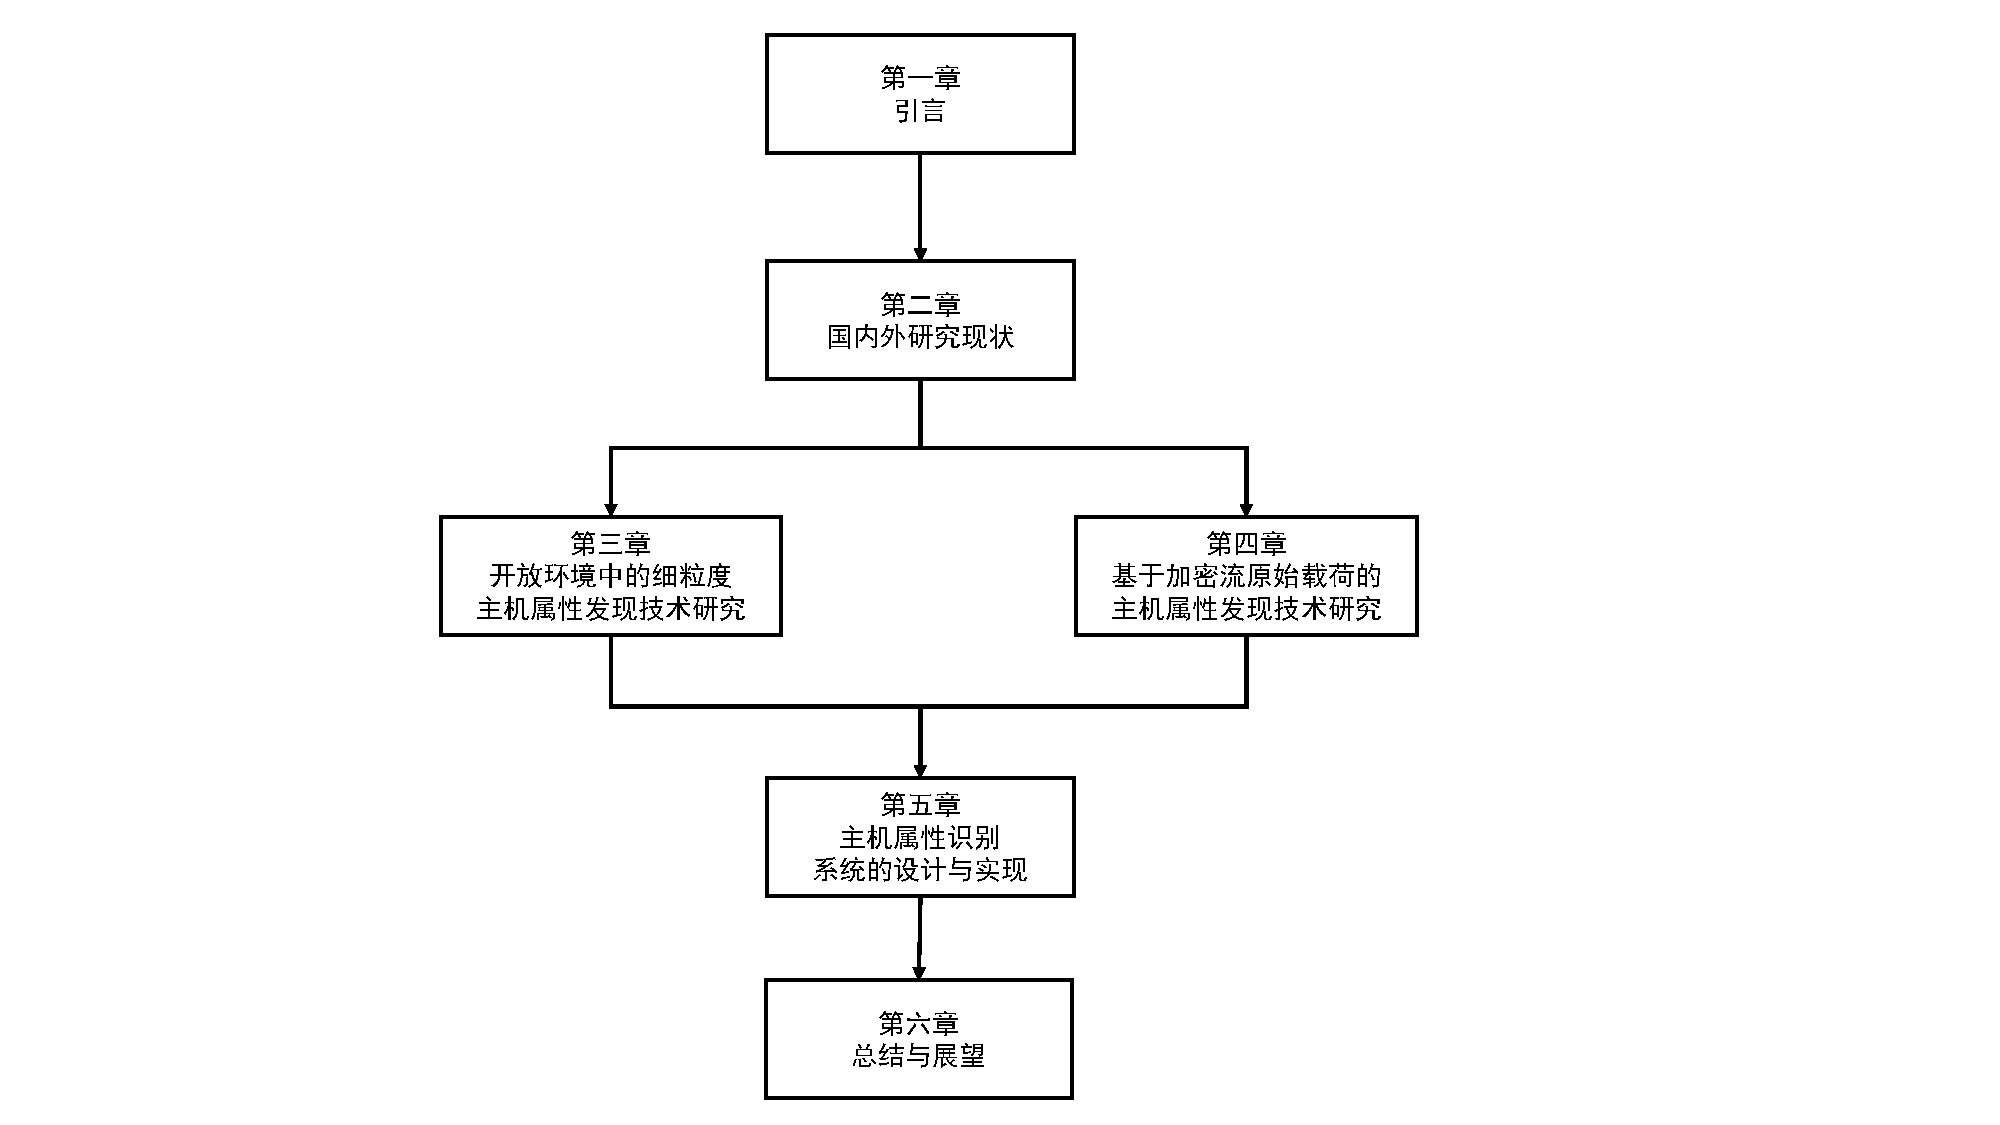
\includegraphics[width=0.8\textwidth]{论文组织结构}
    \bicaption{本文的组织结构}{The structure of this thesis}
\end{figure}

第一章为引言部分,介绍了选题的背景意义、研究内容以及主要贡献,并描述了本文的组织结构。

第二章为国内外研究现状,分别从主动和被动的角度总结了主机属性识别技术的基本原理和研究现状。通过对当前研究成果的总结,发现目前该领域存在的问题,明确本文的研究思路。

第三章为开放环境中的细粒度主机属性发现技术研究,提出了一种基于协议字段特征和流统计特征的主机属性识别方法,着重介绍识别方法的实现细节,包括特征集的选取和机器学习模型效果对比,最终展示识别技术的实验效果。

第四章为基于加密流原始载荷的主机属性发现技术研究,提出了一种利用深度学习模型的主机属性识别方法。此方法基于表示学习的思想,不需要任何先验知识,只需将网络流的原始流数据作为分类器输入,便可完成细粒度的主机属性发现,并拥有更佳的识别效果。

第五章为主机属性识别系统的设计与实现,开发了一套原型系统,可在真实网络中较为准确地识别客户端主机的操作系统类型、版本以及浏览器类型等属性,并具备网络协议识别与解析、TLS流数据属性标注、日志信息存储与查询、主机属性发现实时可视化等功能。

第六章为总结与展望,总结了本文的研究内容与成果,并对未来的研究方向进行了展望。
\chapter{国内外研究现状}

根据获取目标主机网络特征的方式,目前主机属性识别方法可分为主动方法和被动方法两类。因此,本章将从主被动两个角度分别介绍主机属性识别方法的技术思路和研究现状,然后针对目前该领域遇到的问题,明确本文的研究路线,最后对本章内容进行小结。

\section{主动识别方法}

主动识别方法通过构造特定的网络报文发往待测主机,根据待测主机的响应报文推断其主机属性,具有针对性强和准确性高等特点。然而,主动识别行为很容易被入侵检测系统或网络防火墙检测并阻止,经常导致目标主机无法收到探测数据包。因此,主动识别方法仅适用于少量场景。

\begin{figure}[!h]
    \centering
    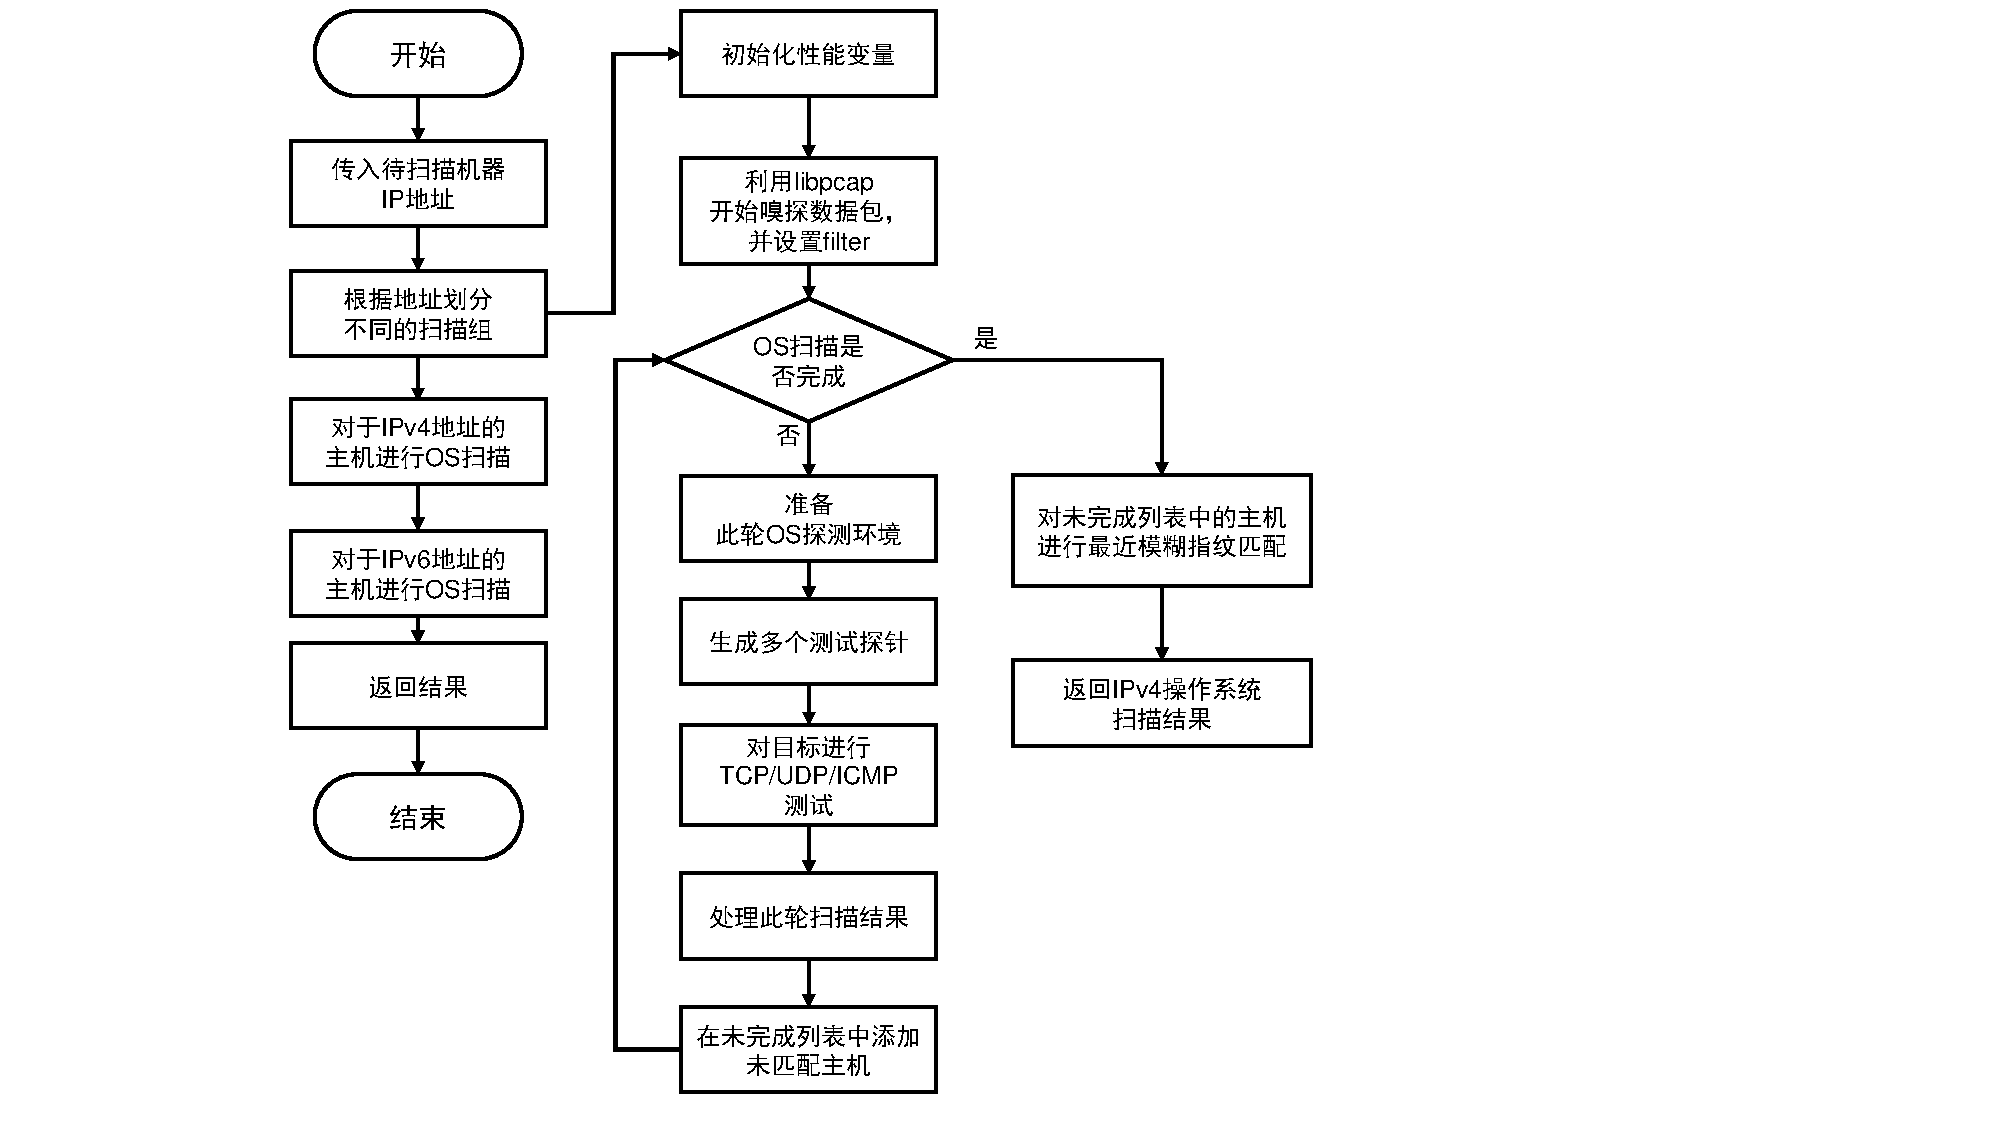
\includegraphics[width=0.7\textwidth]{nmap扫描}
    \bicaption{Nmap扫描流程图}{Nmap scanning flowchart}
\end{figure}

\citet{lyon1998remote}开发了著名的操作系统识别工具Nmap。Nmap工具扫描操作系统信息的流程如图2.1所示,其中网络探针包括6个用于获取序列折时间戳生成信息TCP探针,7个用于扫描开放端口的TCP探针、1个用于扫描关闭端口的UDP探针和2个ICMP探针,以此生成的指纹信息包括TCP时间戳、时钟频率、TCP标志、TCP可选项、IP字段等等。得到TCP/IP协议栈指纹后,Nmap工具会在一个已知系统的指纹数据库中进行匹配,从而获得待测指纹的操作系统信息。最新版本的Nmap同时支持对IPv6地址的主机进行操作系统扫描,其探测原理和IPv4网络中基本相同。该工具的缺点是易被入侵检测系统察觉,并且指纹库的升级需要消耗大量的人力成本。\citet{arkin2002remote}通过对比不同类型操作系统的ICMP协议栈实现,提出了一种基于ICMP报文探针的主动操作系统识别方法,通过向目标主机发送UDP和ICMP协议请求报文获取响应,然后解析响应报文格式得到目标主机的ICMP协议指纹,再借助模糊匹配方法从指纹库中推断目标主机的操作系统类型。该方法在当时解决了某些类型的操作系统因具备相同的TCP/IP协议栈指纹而无法识别的问题,有效提高了操作系统识别技术的准确率。

由于早期的主动操作系统指纹识别工具会向目标主机发送许多数据包,容易被网络防御设备检测,\citet{yarochkin2009xprobe2++}开发了Xprobe2工具,可以优先发送少量探针,降低被发现的可能性。该工具虽然具有模块编程接口,允许添加多种获取信息的网络探针,但默认建议只使用ICMP报文探针。Xprobe2对指纹库采取非严格匹配,对于指纹中的每个字段,分别根据匹配结果进行打分,并最终返回具有最高分数的匹配结果。此外,它还能发送一些针对程序应用层的测试探针。\citet{veysset2002new, beardsley2003snacktime, shamsi2014hershel}相继提出了仅利用单个SYN探针便可识别主机操作系统信息的方法。这些方法基于SYN包和ACK包重传差异,通过时间维度特征来扩展传统的指纹特征集。此类方法在发送探针后,都需要等到相对较长的时间(最多120秒),以便收集SYN包和ACK包重传后的时间差向量信息。

\citet{greenwald2007toward}提出了一种使用更少探针达到高精度识别操作系统的方法,仅需发送一到三个数据包便可获取远程主机的操作系统信息,其精度几乎与Nmap工具通过发送13个探针进行识别的方法一样高。并且他们还发现了TCP窗口大小和TCP可选项是携带特征信息最多的协议字段。同年,\citet{liuying2007ji}首次提出了仅依赖于TCP协议可选项字段的操作系统识别方法,识别原理是不同类型的操作系统对于网络探针的响应数据报文中的TCP可选项序列存在差异。虽然这种方式的探测成功率较高,但是识别的准确率较低。\citet{auffret2010sinfp}首次设计了一种基于IPv6网络进行操作系统识别的工具SinFP,并且此工具既可以进行主动识别,也可以进行被动识别。它首次配备了IPv6指纹库,如果待测指纹在IPv6指纹库中匹配失败,则可以回退到IPv4指纹库中再次进行匹配。为了实现IPv4指纹和IPv6指纹的自动转换,SinFP定义了以下对应关系:IPv4标志对应IPv6流标签,IPv4跳数对应IPv6跳数限制,IPv4分片标志对应IPv6流量类别等。由于操作系统通常在IPv4和IPv6之间共享TCP实现,因此这种转换是合理有效的。此外,SinFP利用启发式方法进行模糊匹配,可以解决部分未知指纹不能识别的问题。同样为了解决Nmap工具不能识别未知操作系统指纹的问题,\citet{zhoutiezheng2011ji}将支持向量机引入Nmap工具,但是该方法识别的操作系统类型范围较小,计算复杂度较高。

\section{被动识别方法}
被动识别技术利用网络监听技术获取目标主机与其他设备的镜像流量,通过从镜像流量中提取所需特征信息,结合数据库匹配方法或者机器学习算法,得到目标主机的属性信息,隐蔽性较强,但准确率相对主动方式较差。按照流量特征种类的不同,被动识别技术可以分为基于明文协议的方法,基于TCP/IP协议栈指纹的方法和基于流统计特征的方法。

\subsection{基于明文协议的方法}

由于早期协议开发未考虑数据安全的重要性,许多被广泛应用的网络协议都是明文协议。在未加密的HTTP协议、DNS协议、SSH协议等应用层协议中,都可以直接获取主机属性信息。例如,在Web应用HTTP流的GET请求报文中,首部的User-Agent字段通常都显式标注了客户端主机的属性信息,包括操作系统类型、版本以及浏览器类型。表2.1列出了部分主机属性与User-Agent字段的对应关系。此类方法的优势是识别速度非常快,准确率较高,但是随着流量加密技术的普及,基于明文信息的识别技术必将逐渐被淘汰。

\begin{table}[!htbp] 
    \bicaption{主机属性和User-Agent对应关系}{Correspondence between host attributes and User-Agent}
%    \label{tab:sample}
    \centering
    \footnotesize
    \setlength{\tabcolsep}{15pt}
    \renewcommand{\arraystretch}{1.2}
\begin{tabular}{cll}
\toprule
类型 & User-Agent字段 & 主机属性信息\\ \hline
\multirow{4}{*}{操作系统} & Windows NT 5.1 &Windows XP\\ 
& Windows NT 6.1 & Windows 7\\ 
& Windows NT 6.2 &Windows 8\\ 
& Windows NT 6.3 &Windows 8.1\\ \cline{2-3}
\multirow{4}{*}{浏览器} & Chrome/74.0.3729.169 & Chrome 74 \\
& OPR/43.0.2442.991 & Opera 43 \\
& Firefox/7.0.1 & Firefox 7 \\
& MSIE 6.0 & Internet Explorer 6 \\
\bottomrule
\end{tabular}
\end{table}

\citet{matsunaka2013passive}首次提出了一种基于DNS流量解析的操作系统识别方法。该方法主要利用各类操作系统的DNS查询特征不同进行识别,例如独特的查询域名,查询模式和时间间隔。虽然实验结果较好,但是该方法没有考虑异常查询行为的可能性。\citet{lastovicka2018passive}在一个大型校园网流量中对比了三种操作系统识别方法。结果表明,基于HTTP协议User-Agent字段的方法识别准确率最高,但识别范围仅能覆盖网络中一小部分主机。相反,基于TCP/IP协议参数的方法具有较广的识别范围,但识别精度较低。同时他们首次提出了一种新的基于特殊域名的识别方法,其性能不弱于前两种方法。此外,\citet{lastovicka2018passive}还测试了新型协议如IPv6和HTTP 2.0等对操作系统指纹识别技术的影响,认为基于HTTP协议User-Agent字段的方法和基于TCP/IP协议参数的方法在未来将不适用,只有基于特定域名的识别方法仍然可行。

\subsection{基于TCP/IP协议栈指纹的方法}

TCP/IP协议栈采用五层网络模型结构,主要包括物理层,数据链路层、网络层、传输层和应用层等。其中,网络层主要采用IP协议,IP协议可以提供无保证的尽可能快的网络传输服务,通过路由器将局域网连接成互联网。传输层主要采用TCP协议和UDP协议,TCP协议提供面向连接的服务,通过交互三次数据包完成连接的建立和相关参数的协商,如图2.2所示。

\begin{figure}[!h]
    \centering
    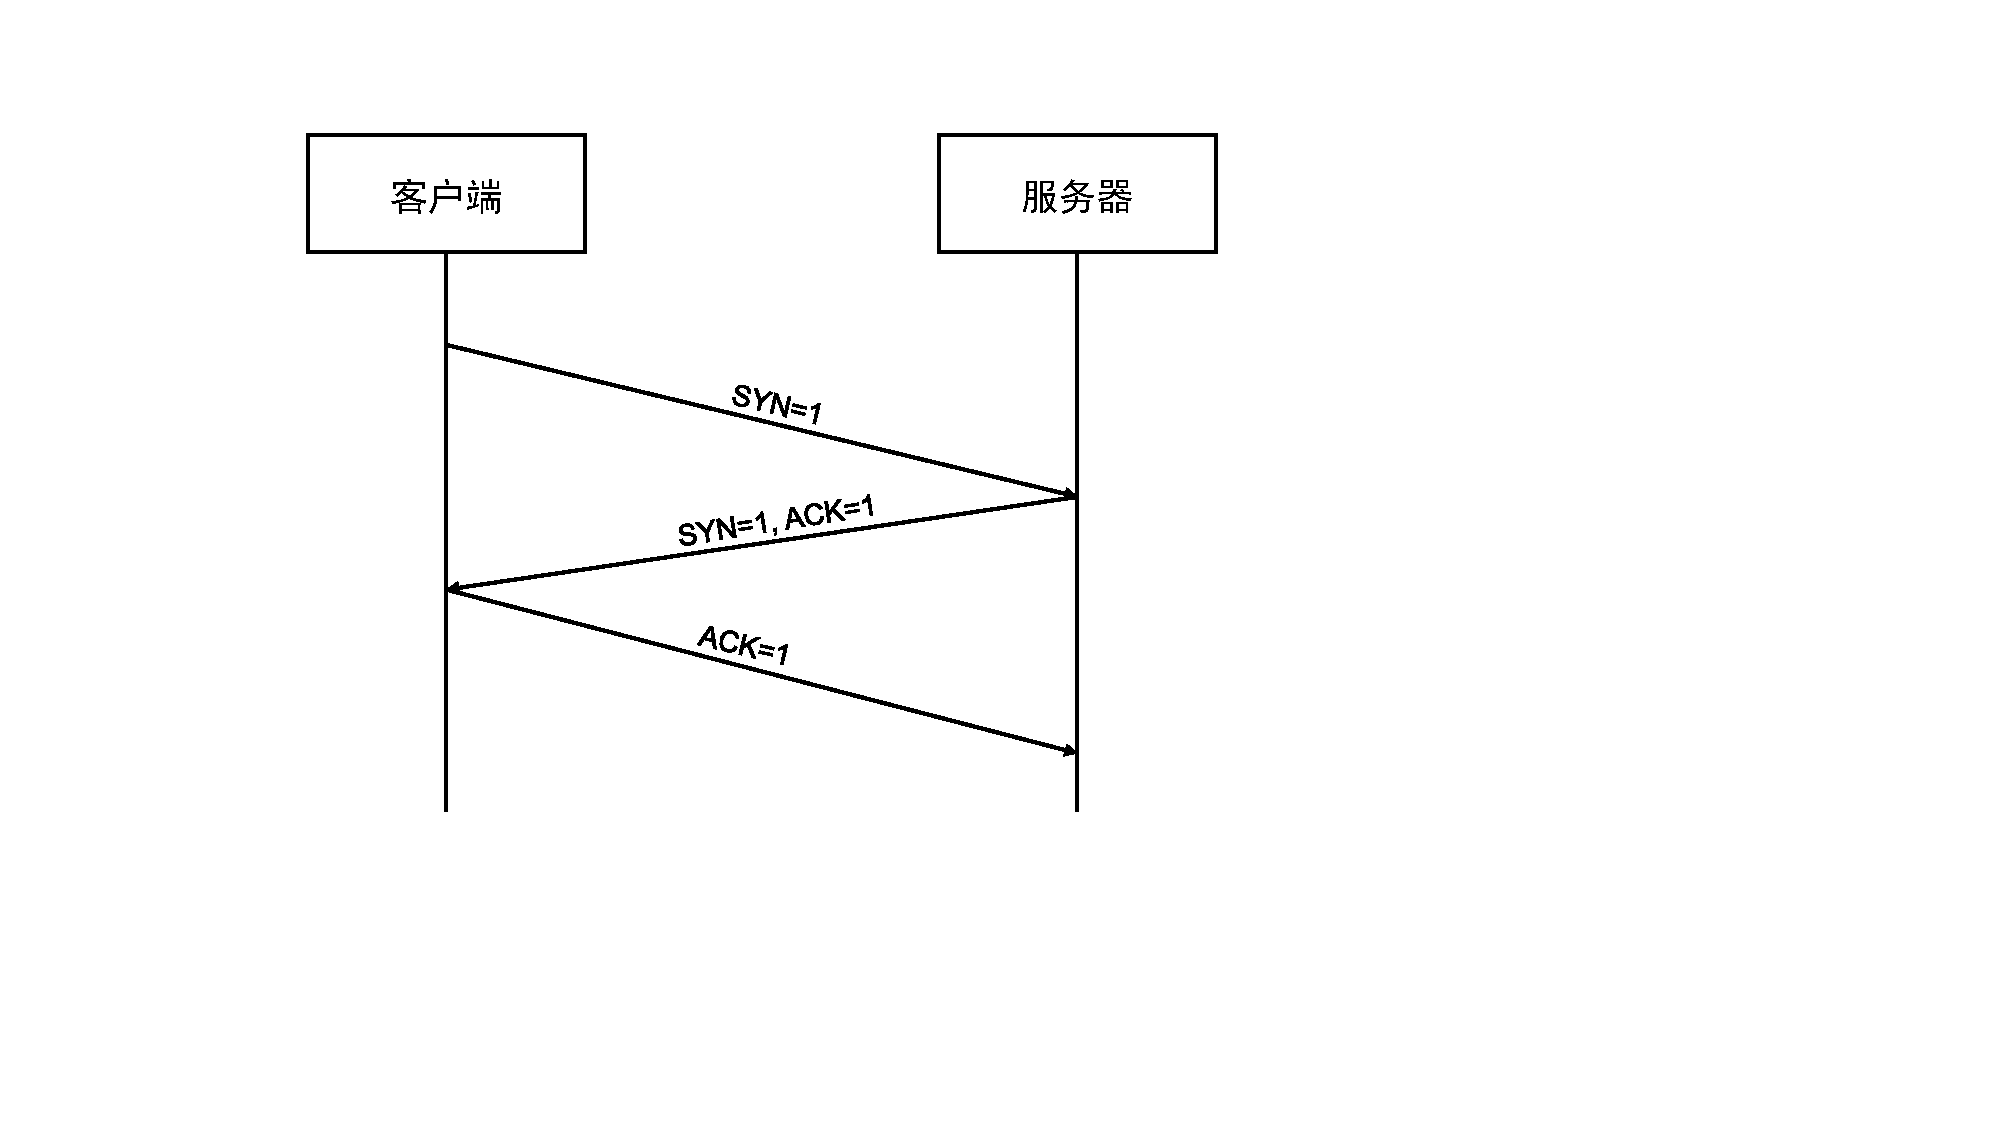
\includegraphics[width=0.5\textwidth]{TCP握手}
    \bicaption{TCP建立连接过程}{TCP connection establishment process}
\end{figure}

三个数据包的具体内容为:客户端首先向服务器发送一个请求建立连接的握手包,SYN字段标识为1,ACK字段标识为0,并附带客户端的协商参数,然后等待对方响应。若服务器正常运行,会回复一个SYN字段和ACK字段都标识为1的响应数据包,数据包附带服务器的协商参数。最后在协商完参数后,客户端会响应一个ACK标识为1的确认数据包,完成本次TCP连接。
 
由于不同属性的主机在实现TCP/IP协议栈时存在差别,称为TCP/IP协议栈指纹,可用于识别客户端的主机信息。TCP/IP协议栈指纹一般取自TCP建立连接过程中的第一个数据包,因为此数据包携带客户端主机的协商参数,如IP协议的分片标识、TCP协议的窗口大小和最大报文长度。表2.2列出了一些常见操作系统在以上参数的区别。

\begin{table}[!htbp] 
    \bicaption{常见操作系统TCP/IP协议栈指纹}{Common operating system TCP / IP protocol stack fingerprint}
    \centering
    \footnotesize
    \setlength{\tabcolsep}{10pt}
    \renewcommand{\arraystretch}{1.2}
\begin{tabular}{ccccc}
\toprule
操作系统 & IP跳数 & IP分片标识 & TCP窗口大小 & TCP最大报文长度\\ \hline
Windows 7 & 128 & 1 & 8192 & 1460 \\
Windows vista  & 64 & 0 & 8192 & 1200 \\
Linux 2.6 & 64& 1& 5792& 1460 \\
Linux 3.0 & 64 & 0 & 32736 & 1414 \\
MAC & 64 & 1& 33304 & 1460 \\
Openbsd & 64 & 1& 32768 & 1460 \\
\bottomrule
\end{tabular}
\end{table}

%TCP/IP协议栈指纹是基于不同属性主机在实现网络协议栈时的差异产生的,具有多样性和稳定性的特点。多样性是指不同属性的设备具备不同的协议栈指纹,稳定性是指同一类型的设备产生的指纹在一定的时期内不发生变化。

\citet{lippmann2003passive}实现了基于TCP/IP数据包头识别9种操作系统的分类器。该分类器主要利用KNN模型和决策树模型进行识别,通过交叉验证实验测试,准确率可以达到90\%。同时,\citet{beverly2004robust}借助概率学习思想,开发了一个朴素贝叶斯分类器,可以被动地从报文首部数据中推断出主机的操作系统类型,并比较了基于机器学习的方法和基于规则的推理工具(例如p0f的指纹数据库)之间的性能差异。最后通过分析一个因特网交换器上的流量,发现所有流量中的大部分流量都由一小部分操作系统产生。此外,作者利用该分类器统计了伪装在NAT设备后面的主机规模,并根据其他技术对结果进行评估,发现网络中由于NAT技术而导致的主机数量增多的比例大约为9\%。\citet{zalewski2006p0f}设计并开发了一套基于TCP/IP协议栈栈指纹的开源工具p0f,利用存储在文本文件中的指纹数据库来识别操作系统。\citet{barnes2013k}在p0f工具的基础上,开发出了k-p0f工具,其基于Linux内核实现,结合高效搜索算法,实现了高吞吐量、高精度的操作系统类型识别。\citet{richardson2010limits}讨论了操作系统指纹自动识别的局限性,提出了操作系统自动检测的四个主要挑战。第一个挑战是当前工具无法为不同的操作系统类型找到可概括样本空间并具有足够区分性的分类规则。其次,全自动工具无法有效利用协议的语义知识挖掘更多信息。最后两个挑战是全自动工具在实际网络中表现不好,并且普遍存在过拟合现象。总而言之,他们认为人工专家知识在未来一段时期内仍然是操作系统指纹生成技术中不可或缺的一部分。

在2014年,多篇关于主机属性识别技术的研究成果发表。\citet{chen2014fingerprinting}基于贝叶斯的规则分析比较了一系列TCP/IP协议首部特征对于操作系统分类任务中的有效性。结果表明,用于识别桌面端操作系统的一些技术并不能用于移动端操作系统的识别。\citet{jirsik2014identifying}提出了一种基于流的高性能操作系统检测系统,可以处理大规模流量。\citet{al2014improving}首次引入TCP FIN包特征,扩展了基于p0f指纹的特征集,可对移动端和桌面端的操作系统进行检测,并且检测的粒度更细。\citet{matouvsek2014towards}通过非监督机器学习中的聚类算法处理新的操作系统协议指纹,使得基于规则的推理方法具备了启发性。此外,还将指纹信息用于增强IPFIX标准记录,以便于大规模检测。

面对加密流量规模快速增长的现象,\citet{husak2016https}认为可以仅利用SSL/TLS握手参数便可识别客户端的主机属性。客户端在建立TLS连接时会发送一个Client Hello包,他们发现客户端在Client Hello包中存在主机标识。其中,最具有区分性的标识是客户端支持的密码套件列表。通过研究密码套件列表和HTTP协议的User-Agent字段之间的关系,提出可以构建密码套件列表和User-Agent信息的映射字典,基于该字典可以实时快速的识别客户端的主机属性,包括操作系统信息和浏览器信息。该研究的实验结果表明,此方法可以识别出95.4%的HTTPS网络流量。而在此之前,\citet{bujlow2015web}调查了当时已知的主机属性扫描技术,提出可以使用代理工具或者通过手动更改机器支持的密码套件列表等方法避免基于SSL/TLS协议指纹的恶意扫描活动。

\citet{tyagi2015packet}利用基于欧几里得距离的分类器可以从大约2000个SYN数据包中正确识别95.5%的数据包的操作系统。同时,\citet{fifield2015remote}通过查阅IPv6协议的的RFC文档,从中找出多处说明不详或未严格定义的协议实现,进而确定了基于IPv6协议字段的操作系统指纹,包括IPv6协议的长度字段,时间戳字段以及跳数限制字段等等。并利用线性分类器进行操作系统指纹的识别。\citet{anderson2017fingerprinting}的研究通过在一个时间窗口内聚合同一客户端发出的多条TLS会话特征,可以高精度地识别操作系统的主要版本和次要版本。\citet{aksoy2017operating}结合遗传思想,利用OneR模型、随机森林模型和J48模型三种机器学习算法对TCP/IP报文头部特征进行了最优特征子集选择。结果表明,遗传算法显著减少了需要分析的报文特征,同时也提高了识别性能。\citet{lavstovivcka2018machine}在计算效率、内存要求、准确率、精度和召回率等方面,比较了四种常用的机器学习方法性能,包括KNN模型,决策树模型,朴素贝叶斯模型和支持向量机模型等。实验结果表明,决策树模型是最适合处理主机属性发现任务的机器学习模型。

由于物联网近些年来得到了巨大的发展,同时继承了传统网络的安全性问题,操作系统识别引起了物联网网络安全性的研究关注。\citet{xuan2018identification}提出了一种基于RIPPER模型的被动操作系统识别方法。通过将其与现有的支持向量机和C45决策树分类算法进行实验对比。结果表明,基于RIPPER的算法具有更好的识别精度和识别效率。

\subsection{基于流统计特征的方法}

随着加密协议和私有协议的广泛应用,包括深度包检测技术在内的流量识别手段在越来越多的场景中失去作用,基于流统计特征的识别方法开始流行。流统计特征主要是指利用一次网络会话中所有数据包的包长、包达到时间以及包方向序列产生的统计值特征,例如最值、均值、均方差等等。此类方法一般需要结合机器学习模型或深度学习模型构建分类器,具有较高的识别准确率。

\citet{ruffing2016smartphone}认为移动设备产生的网络流量的时序特征由该移动设备运行的操作系统决定,提出通过分析网络报文时序的频谱以识别与操作系统相关的频率特性。由于无需利用报文内容,该方法可适用于流量加密的场景。通过收集运行 Android、iOS、Windows Phone和Symbian等操作系统的智能手机产生的流量,在观察时长为5分钟的报文序列后检测率能够达到90\%。然而该方法在判断同一操作系统的不同版本时效果并不理想。\citet{muehlstein2017analyzing}利用会话中每个数据包的长度序列特征和时间序列特征识别操作系统,结合以径向基函数作为内核的支持向量机模型,可以使得操作系统类型识别准确率达到96.06\%。

\section{本章小结}

本章主要从两个方面介绍了主机属性识别技术的研究现状。主动识别技术首先利用网络探针获取目标主机的响应报文,通过解析响应报文中的信息识别目标的主机属性。虽然具备准确率高和针对性强的优点,但易被网络防御设备干扰,适用场景有限。

而被动识别技术不需要和目标主机进行直接交互,只需监听网络中的数据包,通过提取并利用网络数据包中的协议首部信息、载荷信息和其他信息等便可识别目标主机属性。由于被动识别不受防火墙等安全设备的影响,其适用范围更广,缺陷是识别准确率相对较差。根据所需特征种类的不同,被动识别技术又分为基于明文协议的方法,基于TCP/IP协议栈指纹的方法和基于流统计特征的方法。每种方法的优缺点如表2.3所示。

\begin{table}[!htbp] 
    \bicaption{被动识别方法比较}{Comparison of passive identification methods}
%    \label{tab:sample}
    \centering
    \footnotesize
    \setlength{\tabcolsep}{15pt}
    \renewcommand{\arraystretch}{1.2}
\begin{tabular}{ccccc}
\toprule
被动识别方法 & 精度 & 性能 & 加密场景适用性 & 识别粒度\\ \hline
明文协议字段 & 高 & 快 & 否 & 细 \\ 
TCP/IP协议栈指纹 & 低 & 较快 & 是 & 细 \\ 
流统计特征 & 高 & 慢 & 是 & 粗 \\ 
\bottomrule
\end{tabular}
\end{table}

总体而言,当前主机属性识别领域依然存在以下问题:

\begin{itemize}

\item 识别成功率和准确率较低。由于入侵检测技术的日趋成熟,主动识别方法的适用范围越来越窄,成功探测到目标主机属性信息的成功率显著下降。所以未来应着重于研究被动识别方法,弥补其准确率较差的缺陷,从特征集和识别算法两个角度提升被动识别技术的效果和性能。

\item 识别粒度较粗,识别类型较少。大部分研究成果只能识别操作系统类型,无法识别操作系统版本和浏览器信息,而常见网络漏洞与操作系统类型和版本以及浏览器类型都密切相关,为了提高主机属性识别技术的应用价值,需要更细粒度和更广范围的识别方法研究。

\item 人工成本较高。无论是主动还是被动识别方法,主机网络指纹的设计都依赖于较高水平的专家经验,此外,在传统的指纹库匹配方法中,指纹库的更新也需要大量的人力和物力。因此,研究如何借助机器学习模型和表示学习方法识别主机属性具有重要意义。
\end{itemize}

面对上述挑战,本文将从被动角度面向加密网络进行主机属性发现技术的研究,综合当前主机属性识别方法的优点,扩展TCP/IP协议栈指纹,结合机器学习模型和神经网络模型,使得主机属性发现技术的准确率更高、性能更快、人工成本更低。


\chapter{开放环境中的细粒度主机属性发现}\label{chap:First_Point}
本章提出了一种基于协议字段特征和流统计特征的主机属性识别技术,用于在开放的动态网络中精准地识别主机的多维属性。本章首先概述该工作的背景意义、技术原理和思路流程,然后分别介绍识别技术中的关键环节,最终展示识别技术的实验效果。

\section{引言}
%保障网络安全最大的挑战之一就是及时发现漏洞,而绝大部分安全漏洞和隐患都与细粒度的主机属性息息相关。此外,识别网络中主机的多维细粒度属性还可以帮助网络运营者有效地进行网络管理、网络资源分配、网络服务质量优化。探测目标主机的相关属性一般分为主动和被动两种方式,而由于入侵检测技术的成熟,主动探测技术的局限性越来越明显,本章将介绍一种被动探测技术,可以精准、快速的识别加密网络中的细粒度主机属性。

尽管RFC文档已经对TCP/IP协议栈的规范进行了统一,但是不同厂商的软件开发者在实际开发和更新操作系统、浏览器等软件的过程中,由于缺乏协商,对网络协议栈的初始化参数进行了不同的设置。这一现象造成了不同属性的主机在网络会话过程中,存在明显的协议字段参数差异和流统计数据差异,称为TCP/IP协议栈指纹。本章方法以TCP/IP协议栈指纹为基础,结合以LightGBM为代表的机器学习模型,对当前主流的操作系统和浏览器进行识别。

如图3.1所示,本章方法首先从网络中采集TLS加密会话,以双向流为单位,提取每条TLS流的TCP/IP协议字段特征、TLS协议字段特征以及流统计特征,在经过数据处理后作为机器学习模型的输入,最终得到多维主机属性。

\begin{figure}[!htbp]
    \centering
    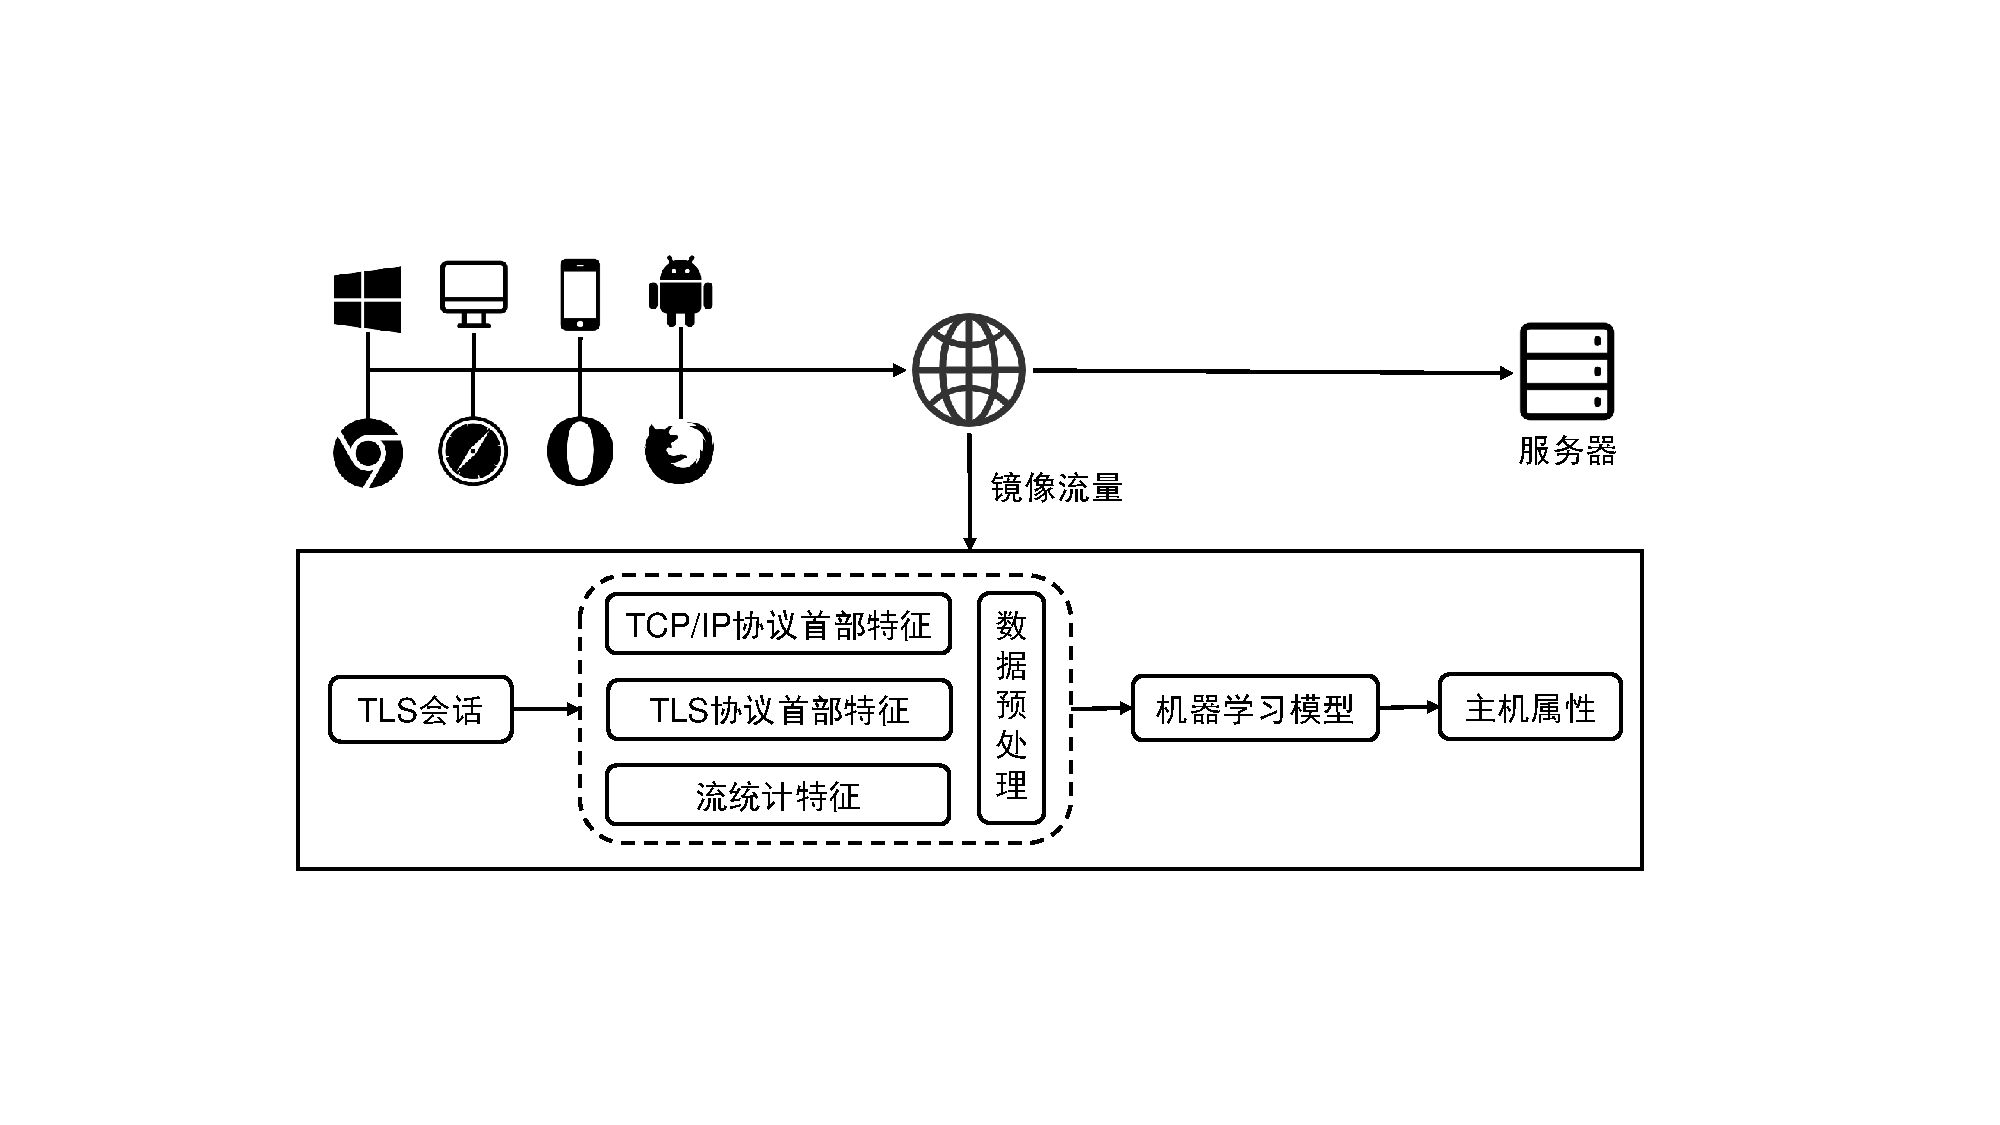
\includegraphics[width=0.9\textwidth]{研究点1结构}
    \bicaption{开放环境中的细粒度主机属性发现技术}{Fine-grained host attribute discovery technology in an open environment}
\end{figure}

\section{特征工程}

在流量识别场景中,单向网络流通常指在一段时间内,具有相同五元组<源地址,目的地址,源端口,目的端口,传输协议类型>的所有数据包形成的包序列。双向网络流由同一时间段内源目地址可互换的单向流组成。本节将介绍以双向流为单位的协议字段特征和流统计特征的提取方法。

\subsection{协议字段特征}

TCP/IP协议栈采用五层网络模型结构,自下向上分别为:物理层,数据链路层、网络层、传输层和应用层。在一次完整的TLS会话中,网络层的主要协议为IP协议,传输层的主要协议为TCP协议。TCP协议是面向连接的协议,一般通过交互三个数据包完成连接的建立。本章从由客户端发往服务端的第一个数据包即TCP SYN包中提取IP协议首部字段和TCP协议首部字段,从TLS Client Hello包中提取TLS协议首部字段。如表3.1所示,本章方法分别从IP协议、TCP协议以及TLS协议首部中提取3维特征、4维特征、6维特征,组成共计13维特征的TCP/IP协议栈指纹。

\begin{table}[!htbp] 
    \bicaption{协议字段特征}{Protocol field features}
    \centering
    \footnotesize
    \setlength{\tabcolsep}{20pt}
    \renewcommand{\arraystretch}{1}
\begin{tabular}{lll}
\toprule
协议 & 特征 & 说明 \\ \hline
\multirow{3}{*}{IP} & time\underline{~~}to\underline{~~}live & 生存时间 \\ 
& total\underline{~~}length & IP包长\\ 
& fragment\underline{~~}flag & 分片标志\\ \hline
\multirow{4}{*}{TCP} & window\underline{~~}size & TCP窗口大小 \\ 
 & window\underline{~~}scale & 窗口缩放因子 \\ 
 & maximum\underline{~~}segment\underline{~~}size & 最大报文长度 \\ 
 & option\underline{~~}type\underline{~~}codes\underline{~~}sequence & 可选项类型序列 \\ \hline
\multirow{6}{*}{TLS} & version & 版本 \\ 
 & dxtensions\underline{~~}length & 扩展长度 \\ 
 & cipher\underline{~~}suite\underline{~~}codes\underline{~~}sequence & 密钥算法套件序列 \\ 
 & extension\underline{~~}type\underline{~~}codes\underline{~~}sequence & 扩展类型序列 \\ 
 & supported\underline{~~}group\underline{~~}codes\underline{~~}sequence & 支持加密组件序列 \\ 
 & ALPN\underline{~~}codes\underline{~~}sequence & 应用层协议协商序列 \\ 
\bottomrule
%random\underline{~~}state & 随机种子 & 6 \\
\end{tabular}
\end{table}

IP报文通常由首部和载荷组成,首部长度可变,通常为20字节,可以根据不同的需要加入各种可选项部分。IP首部的一般格式如图3.2所示,其中,本章方法所提取的IP协议首部参数主要为生存时间,总长度以及分片标志。

\begin{figure}[!htbp]
    \centering
    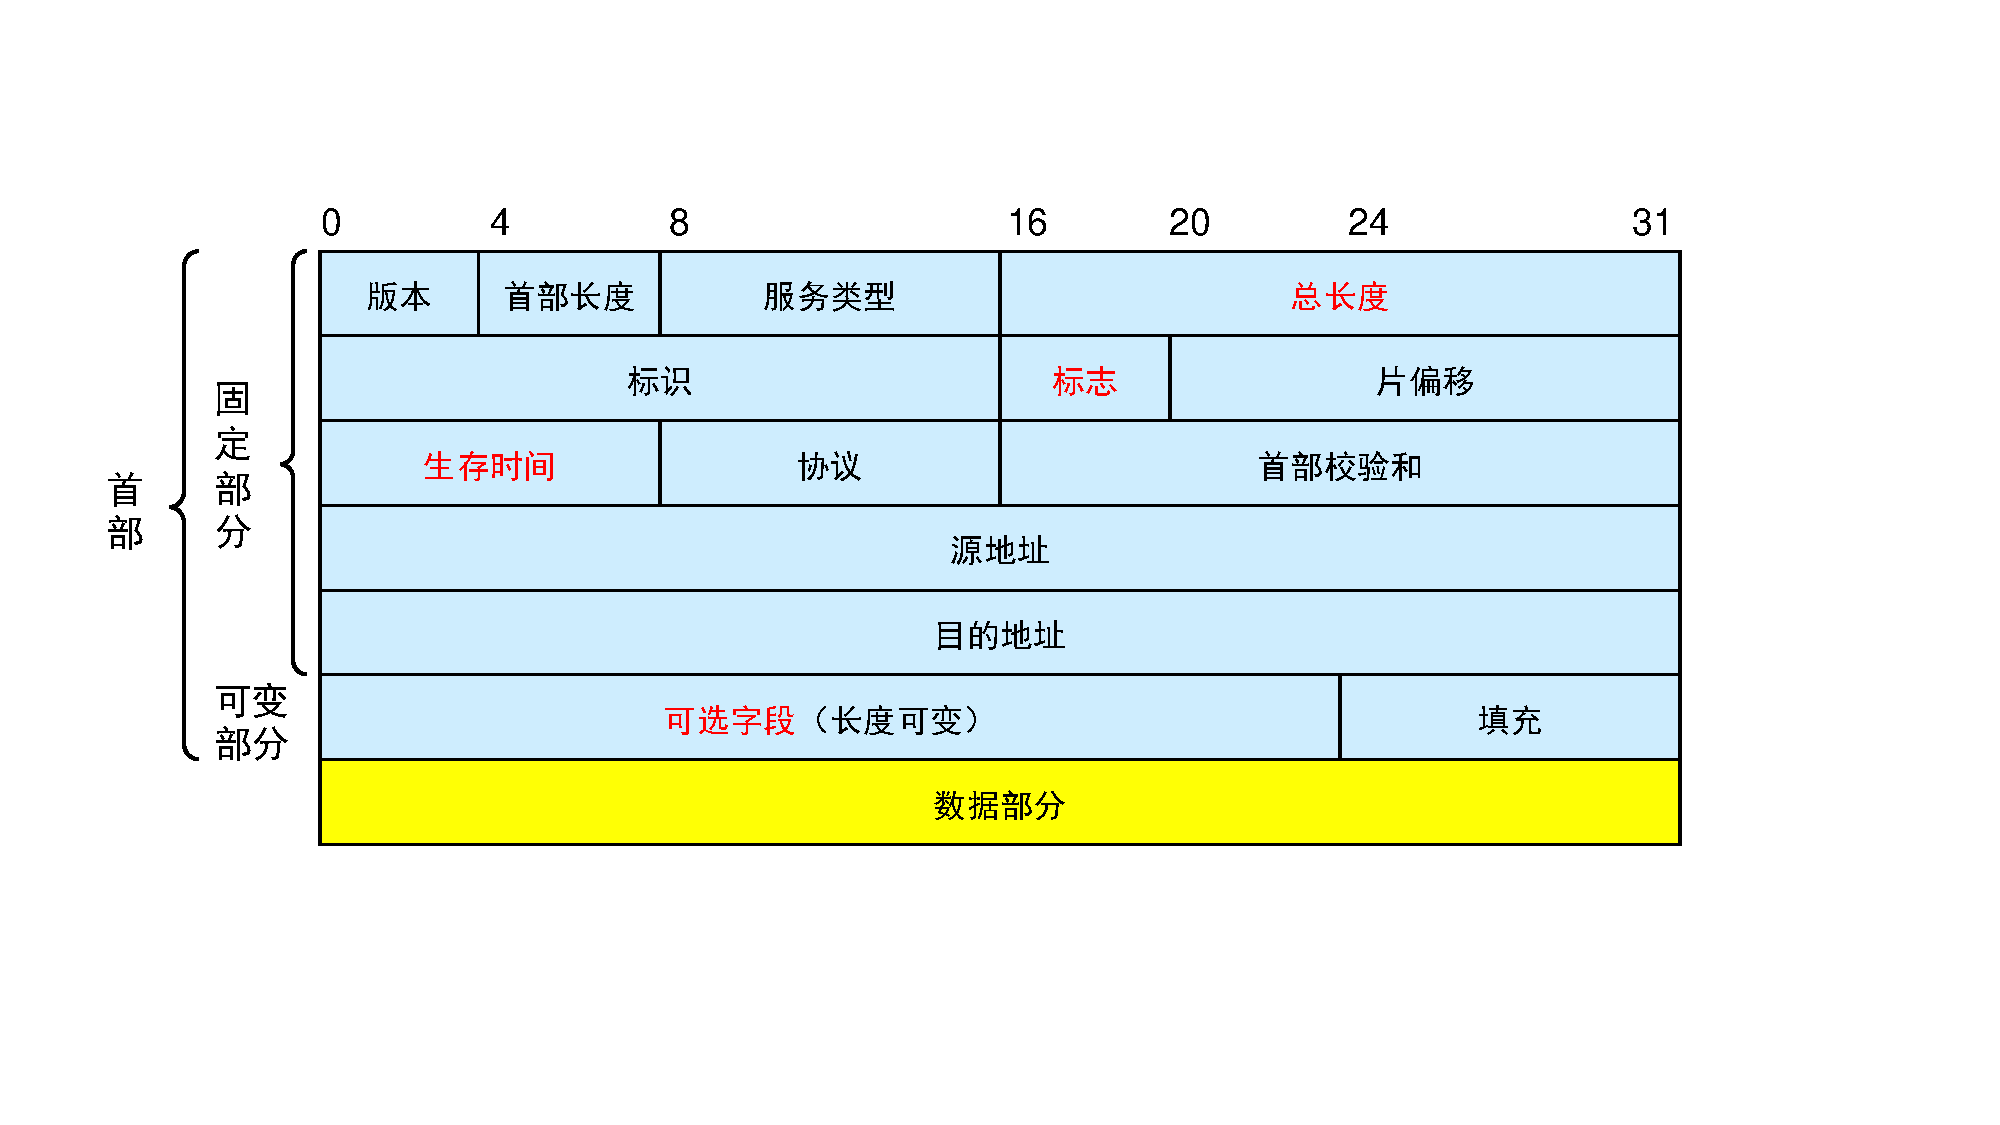
\includegraphics[width=0.9\textwidth]{3-2}
    \bicaption{IP报文格式}{IP protocol format}
    \label{fig:3-2}
\end{figure}

\begin{itemize}
\item 
生存时间(TTL):IP报文所允许通过的路由器的最大数量。每经过一个路由器,TTL减1,当为0时,路由器将该数据报丢弃。TTL字段是由发送端初始设置一个8bit字段,记录了报文在网络中的存活时间,各类操作系统的TTL初始值不同。
\item 
总长度:IP报文的总长度,是报头的长度和载荷的长度之和。
\item 
分片标志:1bit字段,1表示报文不分片,0表示分片。
\end{itemize}

\begin{figure}[!htbp]
    \centering
    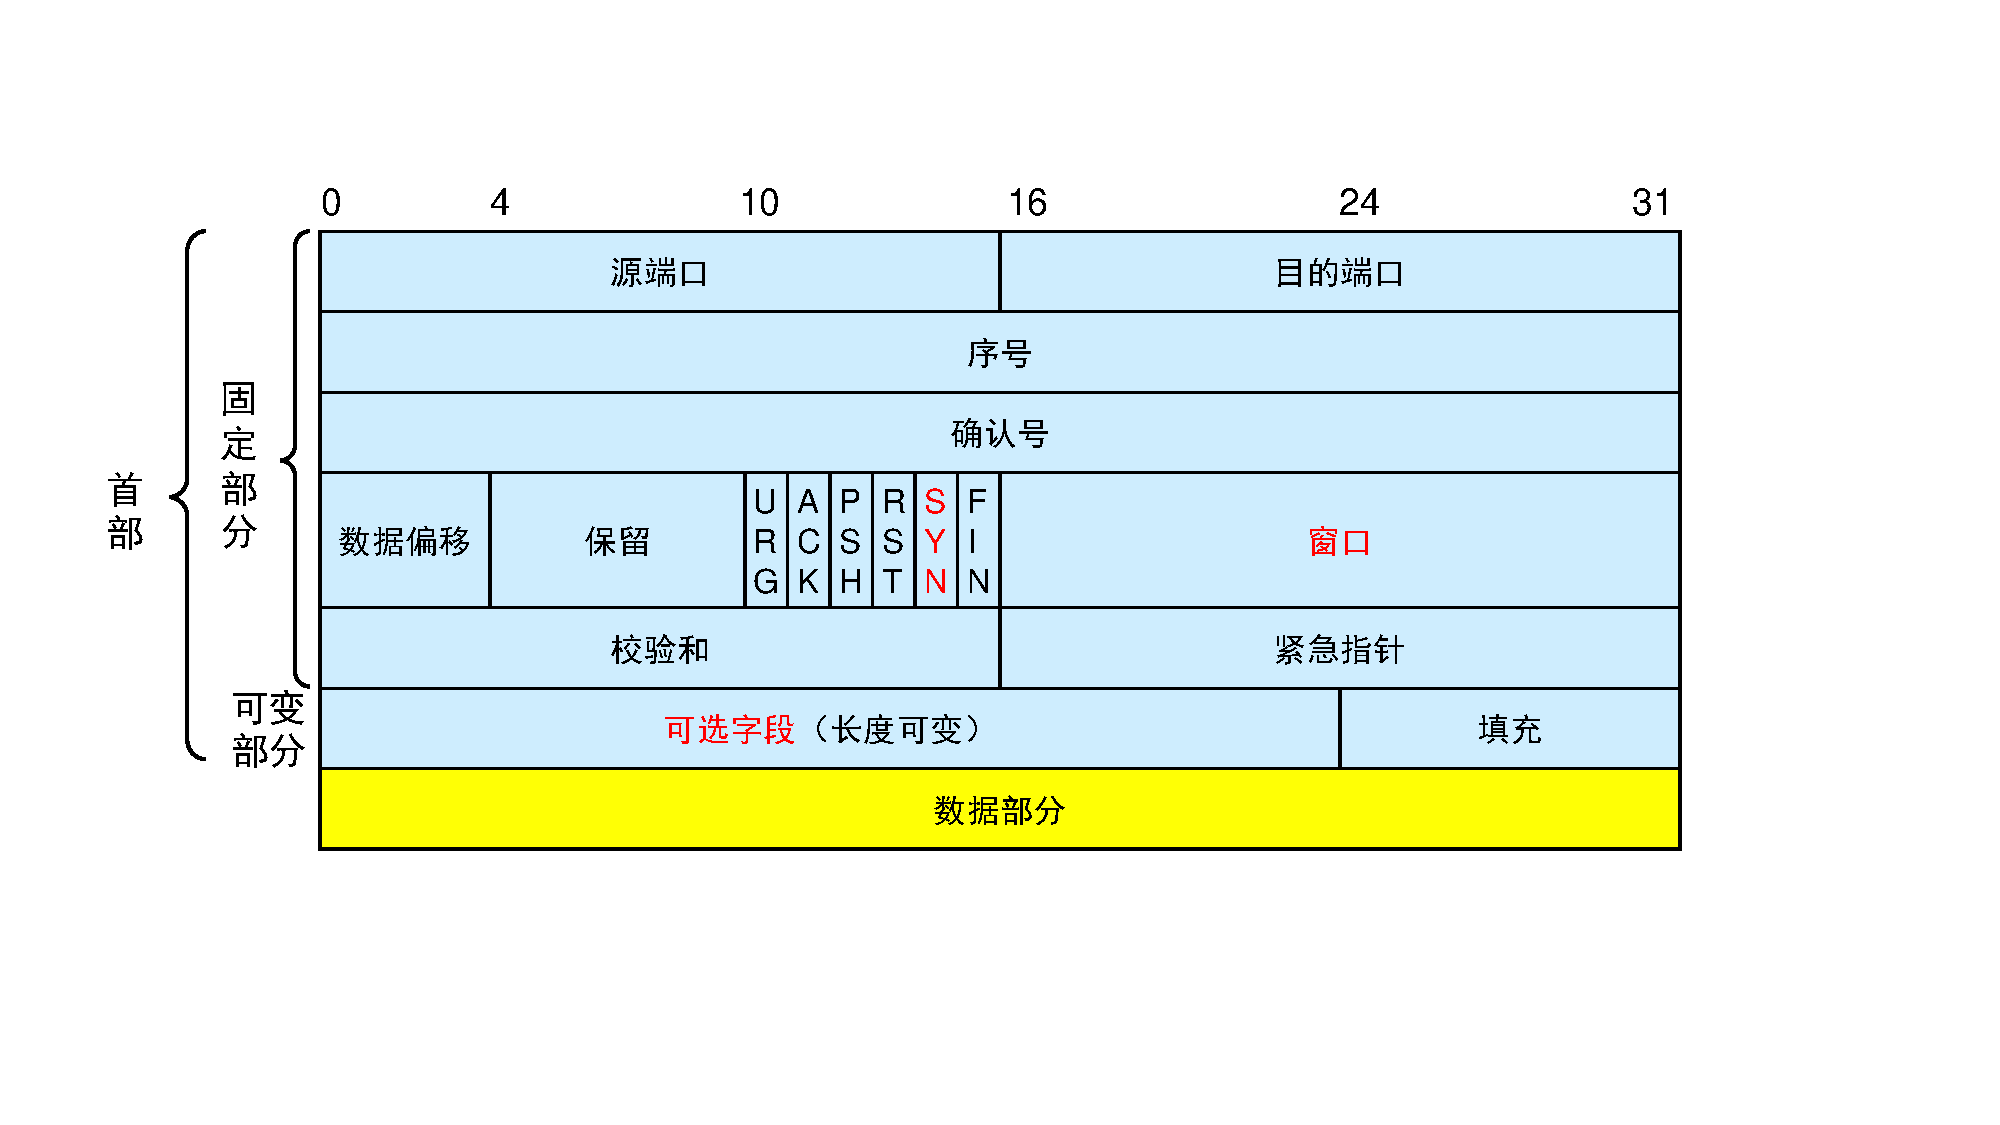
\includegraphics[width=0.9\textwidth]{3-3}
    \bicaption{TCP报文格式}{TCP protocol format}
    \label{fig:3-3}
\end{figure}

TCP报文同样由首部和载荷组成,首部长度一般为20字节,可以扩展不同的可选项部分。TCP首部的一般格式如图3.3所示。其中,本章方法所提取的TCP协议首部参数主要为窗口大小,窗口缩放因子,最大报文长度以及可选项类型序列。

\begin{itemize}
\item 
窗口大小:用来告知对端本地的缓存大小,以此控制对端发送数据的速率,从而达到流量控制的目的。窗口大小为一个16bit字段,因而最大为65535。
\item 
窗口缩放因子:用于提高传输窗口的上限。
\item 
最大报文长度:每一个TCP报文段中数据字段的最大长度。其值太大或太小都不合适,太小会使得数据传输效率很低,太大会增加网络丢包的可能性,增大网络开销。
\item
可选项类型序列:按照字节顺序解析TCP SYN包的可选项字段,从中提取出每一个可选项子字段的类型,并按照一定的编码方式将其转换为类型码,便可得到有序的类型码序列。在本章方法的编码方式中,将NOP类型记作0,最大报文长度类型记作1,窗口缩放因子类型记作2,选择确认项类型记作3,时间戳类型记作4,其他类型记作5。最终得到的类型序列一般形式为$opt\underline{~~}seq=< o_{1},o_{2},o_{3},...,o_{n} >,o_{i}∈[0,5]$。
\end{itemize}

\begin{figure}[!htbp]
    \centering
    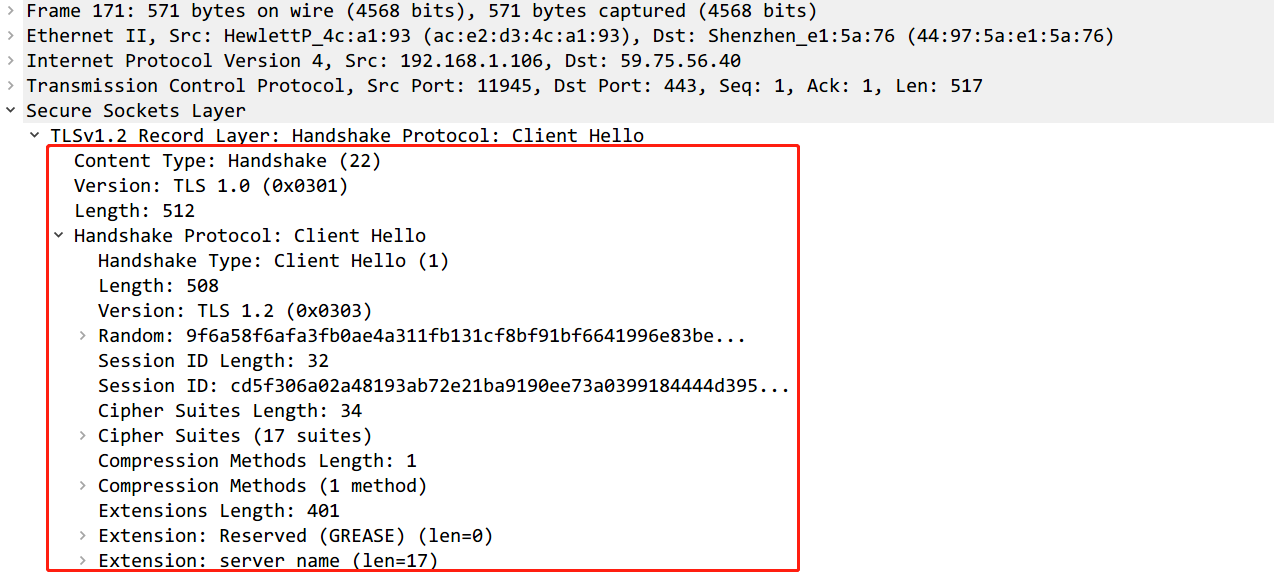
\includegraphics[width=0.9\textwidth]{3-4}
    \bicaption{TLS报文格式}{TLS protocol format}
    \label{fig:3-4}
\end{figure}
TLS Client Hello报文是TLS建立会话的第一个数据报文,本章方法提取的报文首部字段主要有协议版本,密钥算法套件序列,扩展长度,扩展类型序列,支持加密组件序列以及应用层协议协商状态码序列。其报文格式如图3.4所示。

\begin{itemize}
\item 
协议版本:表示客户端支持的最佳TLS协议版本。
\item 
密钥算法套件序列:由客户端支持的所有密钥算法套件组成的状态码序列。加密套件包含客户端能够支持的加密方式、算法等信息。不同的加密套件性能存在差异,同时会产生不同的TLS交互报文。
\item 
扩展长度:TLS协议的扩展部分长度。
\item 
扩展类型序列:TLS协议的扩展部分由任意数量的不同扩展组成。每一类扩展都有一个独特的类型码,按字节顺序解析扩展部分的所有扩展,即可得到扩展类型序列。
\item 
支持加密组件序列:按字节顺序解析,得到Supported Groups扩展字段中的类型码序列。
\item 
应用层协议协商状态码序列:按字节顺序解析,得到Application Layer Protocol Negotiation扩展字段中的类型码序列。
\end{itemize}

\subsection{流统计特征}

流统计特征可以轮廓性地描述不同属性的主机在网络通信过程中的差异。以每条流前50个包的长度序列和时间间隔序列为基础,分别提取网络流在空间、时间以及速率等三个维度的统计特征。空间特征主要包括总包数、总字节数、包长均值、包长均方差、包长直方图分布和包长马尔可夫状态转移矩阵等。时间特征主要包括间隔均值、间隔均方差、间隔直方图分布和间隔马尔可夫状态转移矩阵等。速率特征主要包括包数吞吐量均值、字节数吞吐量均值以及传输峰值分布等。

\begin{itemize}
\item 
包长直方图分布:假设IP协议的最大传输单元为1500字节,设置组数为10,组距为150字节。根据包长序列统计前50个数据包的包长在每个分组中的频数,可得到长度为10的包长直方图分布。
\item 
间隔直方图分布:类似包长直方图分布,以毫秒为单位,将包到达时间间隔分为10组,组距为100毫秒,其中最后一组的组距为[ 900, Inf )。根据包到达时间间隔序列统计其在每个分组中的频数,可得到长度为10的间隔直方图分布。
\item 
包长马尔科夫状态转移矩阵:以包长直方图分布为基础,对每个分组按从小到大分配状态码1到10,根据包长在直方图中的分布便可得到每个包对应的包长状态码。初始化一个10*10的全0矩阵,行号表示前一个数据包的包长状态,列号表示后一个数据包的包长状态,依次统计前50个包的包长状态转移概率,可得到包长序列的马尔科夫状态转移矩阵。
\item 
间隔马尔科夫状态转移矩阵:同样,以间隔直方图分布为基础,对每个分组按从小到大分配状态码1到10,根据相邻数据包的时间间隔在直方图中的分布便可得到对应的间隔状态码。初始化一个10*10的全0矩阵,行号表示间隔序列中前一个间隔状态,列号表示后一个间隔状态,依次统计前50个包的时间间隔状态转移概率,可得到间隔马尔科夫状态转移矩阵。
\end{itemize}

\section{机器学习模型构建}

无论在主动或者被动的主机属性发现技术中,传统方法一般是首先获取TCP/IP协议字段初始值以生成指纹,然后将获得的指纹与预先生成的已知主机属性指纹库中的指纹进行对比,当待识别指纹与已知指纹完全匹配时,便可得到具体的主机属性。传统方法属于静态方法,优点是识别速度快,缺点是无法识别不在指纹库中的未知指纹。为了克服以上缺陷,本章将构建五类经典的机器学习模型用于识别所有指纹的主机属性,提高识别方法的灵活性、准确性和鲁棒性。这五类机器学习模型分别为逻辑回归(Logistics Regression, LR)模型、最近邻居(K-nearest Neighbour, KNN)模型、随机森林(Random Forest, RF)模型、XGBoost模型以及LightGBM模型。

\subsection{逻辑回归模型}

逻辑回归算法是基于线性回归算法的改进算法,也是解决二分类问题的首选方法,在将其推广到多项逻辑回归算法后,可用于多分类任务。与线性回归模型相似,LR模型首先计算每个输入特征的权重,即系数值。然后利用Logistic函数对线性输出值进行非线性变换,使得最终的预测输出值介于0到1之间。模型优点是计算成本小,易于理解和实现。缺点是易出现欠拟合问题,分类精度可能不高。结合网格搜索策略和交叉验证法,逻辑回归模型的最优参数组合如表3.2所示。

\begin{table}[!htbp] 
    \bicaption{逻辑回归模型参数选择}{Logistic regression model parameter selection}
%    \label{tab:sample}
    \centering
    \footnotesize
    \setlength{\tabcolsep}{20pt}
    \renewcommand{\arraystretch}{1.2}
\begin{tabular}{lll}
\toprule
参数 & 含义 & 取值 \\ \hline
penalty & 正则项选择 & l1 \\ 
solver & 损失函数的优化方法 & liblinear \\ 
max\underline{~~}iter & 算法收敛的最大迭代次数 & 4000\\ 
multi\underline{~~}class & 多分类方法 & multinomial \\ 
%random\underline{~~}state & 随机种子 & 6 \\
\bottomrule
\end{tabular}
\end{table}

\subsection{最近邻居模型}

KNN模型是一种用于分类和回归的非参数统计方法。算法的原理是假设相同类别样本之间的相似度更高,可以通过计算与已知类别样本的相似度,来评估未知类别样本可能的分类,是一种基于实例的学习算法。参数K的取值、样本之间的距离度量算法以及分类决策规则是KNN算法的三要素。KNN模型的优点是精度高,对异常值不敏感。缺点是计算复杂度和空间复杂度较高。最近邻居模型的最优参数组合如表3.3所示,其中K值为7。

\begin{table}[!h] 
    \bicaption{最近邻居模型参数选择}{Nearest neighbor model parameter selection}
%    \label{tab:sample}
    \centering
    \footnotesize
    \setlength{\tabcolsep}{20pt}
    \renewcommand{\arraystretch}{1}
\begin{tabular}{lll}
\toprule
参数 & 含义 & 取值 \\ \hline
n\underline{~~}neighbors & KNN模型中的k值 & 7 \\ 
weights & 每个样本的近邻样本的权重 & distance \\ 
algorithm & 限定半径最近邻法使用的算法 & auto\\ 
metric & 距离度量算法 & minkowski \\ 
\bottomrule
\end{tabular}
\end{table}

\subsection{随机森林模型}

决策树是机器学习中的基础模型,它表示样本类别与样本属性值之间的一种映射关系。树中每个节点表示某类样本,每个分叉路径代表某个可能的属性值,而每个叶节点则表示从根节点到叶节点所需路径对应的属性值集合。RF模型作为基于Bagging思想的集成学习算法,是一种包含多个决策树的分类模型,其输出类别由所有树输出的类别众数而定,因此抗过拟合能力较强。RF模型的最优参数组合如表3.4所示,决策树的生长策略基于Gini系数。

\begin{table}[!h] 
    \bicaption{随机森林模型参数选择}{Random forest model parameter selection}
%    \label{tab:sample}
    \centering
    \footnotesize
    \setlength{\tabcolsep}{20pt}
    \renewcommand{\arraystretch}{1}
\begin{tabular}{lll}
\toprule
参数 & 含义 & 取值 \\ \hline
n\underline{~~}estimators & 决策树的数量 & 1500 \\ 
max\underline{~~}features & 特征子集中的特征数目 & auto \\ 
%max\underline{~~}depth & 树的最大深度 & None\\ 
min\underline{~~}samples\underline{~~}split & 节点最小分割的样本数 & 3 \\
criterion & 树的切分策略 & gini\\ 
bootstrap & 是否有放回的采样 & true\\ 
%random\underline{~~}state & 随机种子 & 5 \\
\bottomrule
\end{tabular}
\end{table}

\subsection{XGBoost模型}
XGBoost模型是一种提升树集成模型,属于梯度提升树(GBDT)模型的范畴,基学习器一般选择CART回归树模型,但也可以选择其它类型的模型如逻辑回归算法等。GBDT算法的基本思想是让新的基学习器去拟合前面学习器的偏差,从而不断将加法模型的偏差降低。相对比GBDT算法,XGBoost模型将目标函数进行了二阶泰勒展开,同时加入更多的正则项以及其他改进,显著提升了模型效果和性能。优点是分类精度非常高,缺点是计算代价较大。XGBoost模型的最优参数组合如表3.5所示。

\begin{table}[!h] 
    \bicaption{XGBoost模型参数选择}{XGBoost model parameter selection}
%    \label{tab:sample}
    \centering
    \footnotesize
    \setlength{\tabcolsep}{20pt}
    \renewcommand{\arraystretch}{1.2}
\begin{tabular}{lll}
\toprule
参数 & 含义 & 取值 \\ \hline
booster & 基学习器 & gbtree \\ 
early\underline{~~}stopping\underline{~~}rounds & 早期停止迭代次数 & 1500 \\ 
eta & 学习率 & 0.15 \\ 
min\underline{~~}child\underline{~~}weight & 叶子节点最小权重的和 & 0.7 \\ 
max\underline{~~}depth & 每棵树的最大深度 & 9 \\
subsample & 每棵树的随机样本采样比例 & 0.4 \\ 
colsample\underline{~~}bytree & 每棵树随机采样的特征比例 & 0.7 \\ 
alpha & L1正则化项的权重 & 0.5 \\ 
%seed & 随机种子 & 5 \\
\bottomrule
\end{tabular}
\end{table}

\subsection{LightGBM模型}
与XGBoost模型相同,LightGBM模型也是一种提升树集成模型,属于梯度提升树模型的范畴。但由于采用了Histogram算法,LightGBM模型比XGBoost模型更强大、速度更快。Histogram算法的基本思想是先把连续的浮点特征值离散化成k个整数,同时构造一个宽度为k的直方图。在遍历数据的时候,根据离散化后的值作为索引在直方图中累积统计量,当遍历完一次数据后,直方图便累积了需要的统计量,然后根据直方图的离散值,遍历寻找最优的分割点。该算法大幅降低了模型的内存消耗,显著提升了计算性能。此外,LightGBM模型采用带有深度限制的叶子生长算法代替了传统的决策树生长策略,防止过拟合现象的出现。而且通过优化对类别特征的支持,使得输入特征无需进行One-Hot编码处理。表3.6展示了LightGBM模型经过调参后的最优参数组合。

\begin{table}[!htbp] 
    \bicaption{LightGBM模型参数选择}{LightGBM model parameter selection}
%    \label{tab:sample}
    \centering
    \footnotesize
    \setlength{\tabcolsep}{20pt}
    \renewcommand{\arraystretch}{1}
\begin{tabular}{lll}
\toprule
参数 & 含义 & 取值 \\ \hline
learning\underline{~~}rate & 学习率 & 0.05 \\ 
boosting\underline{~~}type & 模型所用算法 & gbdt \\ 
%application & 模型用途 & multiclass \\ 
max\underline{~~}depth & 每棵树的最大深度 & 10 \\ 
num\underline{~~}leaves & 叶子节点数 & 512 \\ 
max\underline{~~}bin & bin的最大数量 & 500 \\ 
%min\underline{~~}data\underline{~~}in\underline{~~}leaf & 叶子节点中最小样本数 & 20 \\ 
num\underline{~~}boost\underline{~~}round & 迭代次数 & 500 \\ 
\bottomrule
\end{tabular}
\end{table}

\section{数据集构建}

本文于2019年5月6日到2019年5月10日持续五天在中国科技网中采集了约645万条网络流数据(包含了约96万台客户端主机发起的117万次HTTP会话和528万次TLS会话),称为原始数据集。由于主机属性发现任务属于监督学习任务,而获取的原始TLS会话数据缺少主机属性标签,因此本文采集了HTTP会话数据用于对TLS会话数据的属性标注。

\subsection{属性标注} 

在HTTP会话的请求报文中,通常存在一个首部字段User-Agent,它是一个特殊字符串,作用是使得服务器能够识别客户端主机的各种标识信息,如操作系统类型及版本、浏览器类型及版本、浏览器语言等,如图3.5所示。因此可利用HTTP报文的User-Agent字段对TLS会话数据集进行属性标注。

\begin{figure}[!h]
    \centering
    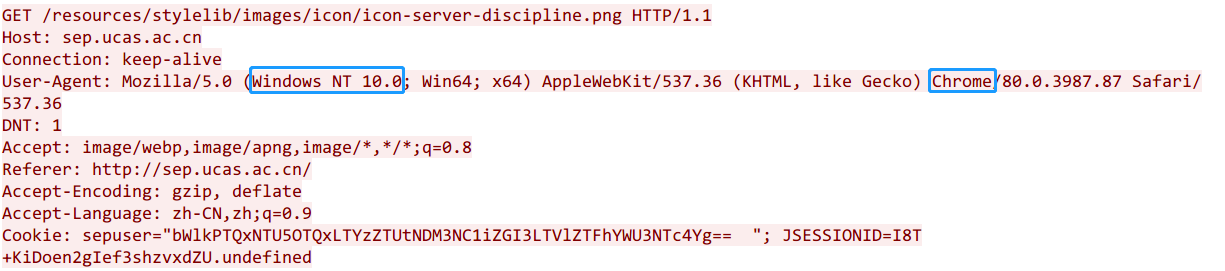
\includegraphics[width=0.9\textwidth]{3-5}
    \bicaption{HTTP协议请求报文中的User-Agent字段}{User-Agent field in HTTP request packet}
\end{figure}

\vbox{}

对于TLS会话数据集中的所有客户端IP地址,通过解析其发送的HTTP请求报文,可得到该IP地址对应的主机属性,并以键值对的形式将以上信息存储到一个主机属性标签字典中。当得到所有客户端IP的主机属性后,便完成了该字典的创建。然后通过查阅主机属性标签字典,可对原始数据集中的所有TLS流样本进行属性标注,得到用于训练机器学习模型的标注数据集。

然而,由于受到NAT和DHCP等网络技术的影响,在一段时间内同一IP可能会被多种内网设备共享,导致从该IP发起的多条HTTP流中解析出不同种类的主机属性,使得单一IP被关联多个标签,无法对该IP发起的TLS会话数据进行有效的属性标注。因此,为了提高属性标注方法的准确性,本文利用同一主机的初始TTL值、操作系统信息和浏览器信息具备不变性这一特征,对主机属性标签字典进行清洗,如图3.6所示。最终,本章构建的标注数据集大约包含401万条TLS会话样本,占原始TLS数据集规模的76\%。

\begin{figure}[!htbp]
    \centering
    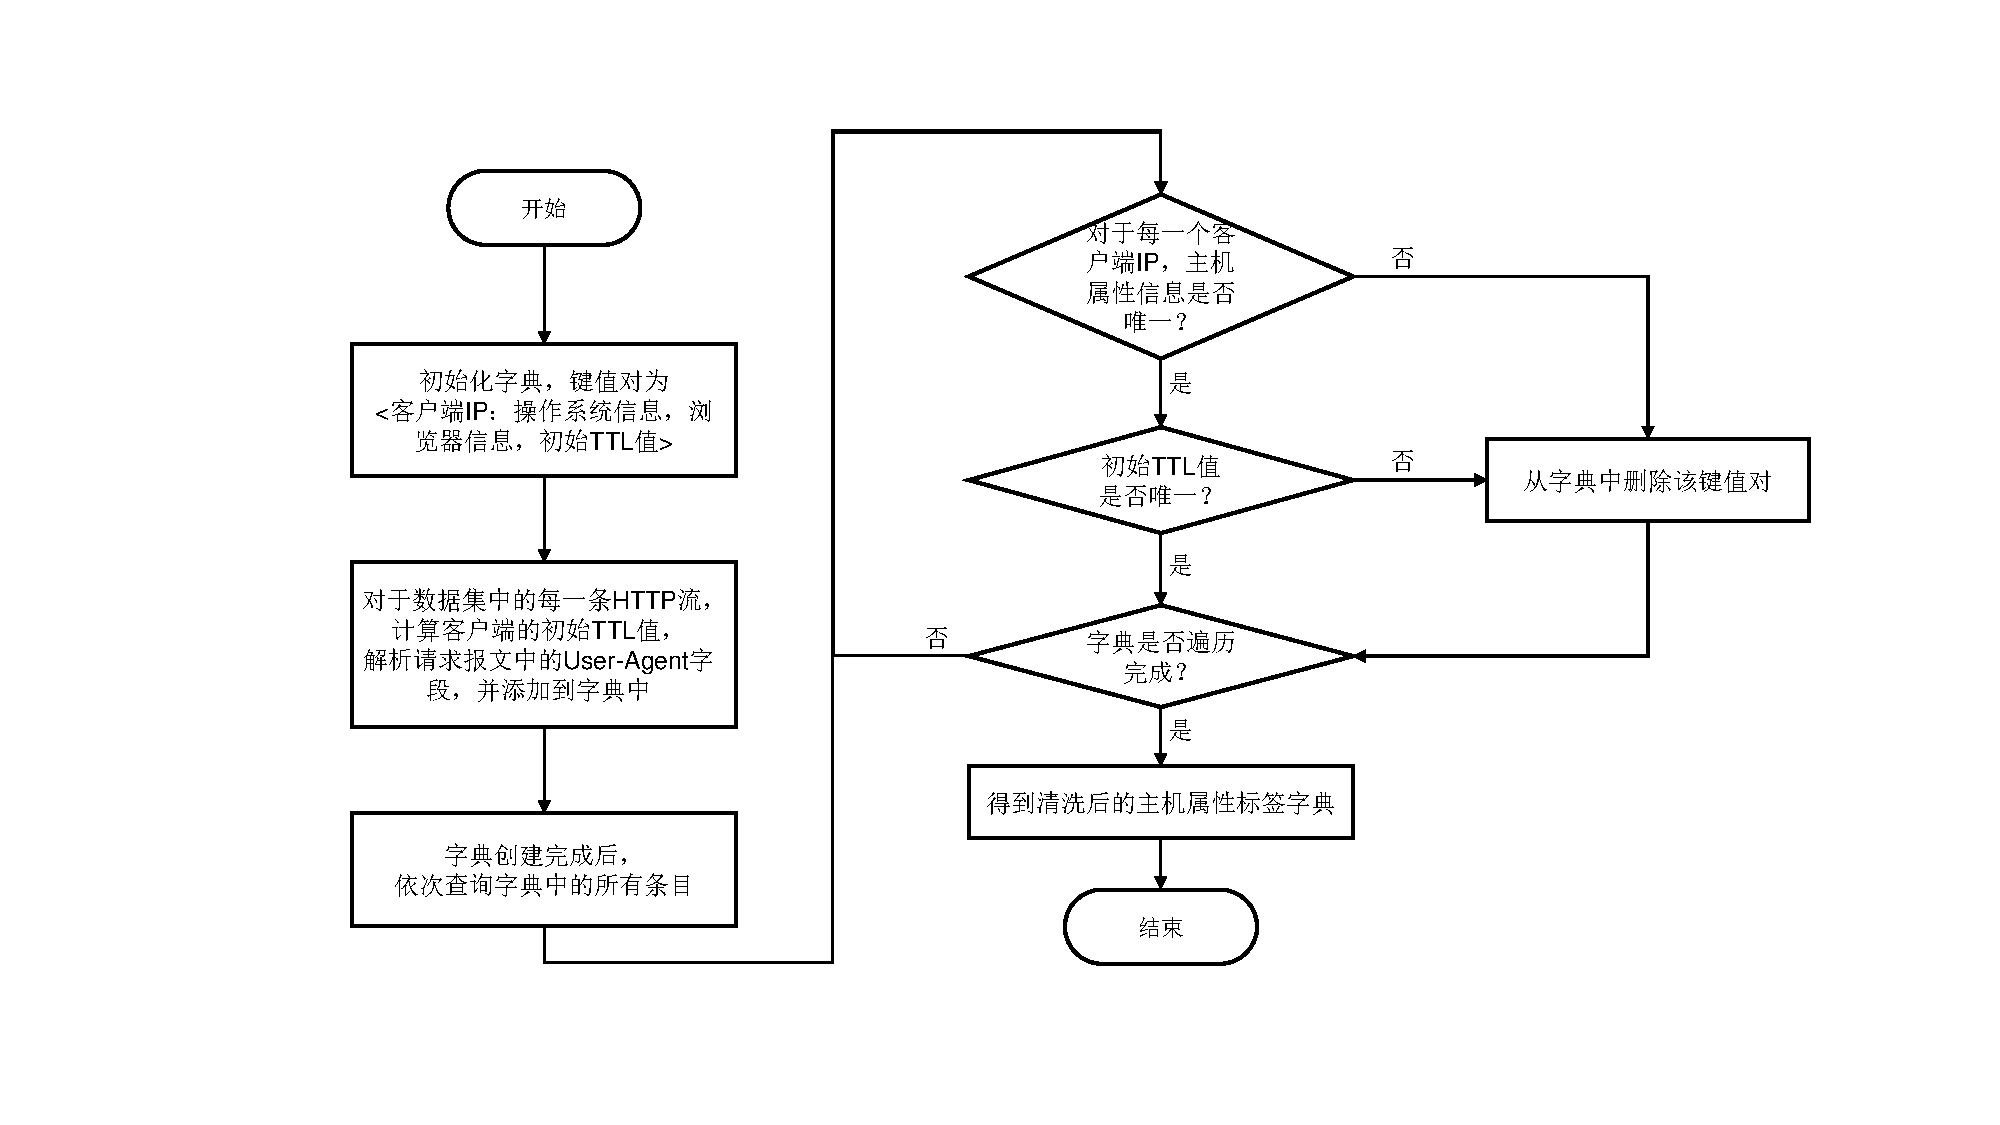
\includegraphics[width=0.9\textwidth]{属性标注方法}
    \bicaption{构建主机属性标签字典流程}{Build host attribute tag dictionary process}
\end{figure}

\subsection{数据集中的主机属性分布} 
经过统计,标注数据集中共包含了5种操作系统类型,21种操作系统主版本以及5种浏览器类型。操作系统类型主要有Android、iOS、Windows、MacOS以及Linux等,浏览器类型主要有Firefox、Safari、IE、Chrome以及Opera等。

在操作系统类型方面,如图3.7(a)所示,Android系统和Windows系统的设备数量最多,占比分别为53.3\%和37.7\%。其次是Apple公司的iOS系统和MacOS系统,共计占比约7.7\%。而Linux系统占比最少,仅为1.4\%。

如图3.7(b)所示,在各类操作系统主版本中,Android 6、Android 7、Android 8和Windows 7等系统版本的数量占比最多。此外,由于从HTTP协议的User-Agent字段中无法识别更多Linux系统的主版本信息,因此本文仅研究最流行的桌面Linux发行版即Ubuntu系统的是识别技术。

在浏览器属性方面,如图3.7(c)所示,谷歌公司的Chrome浏览器和Apple公司的Safari浏览器在数据集中占比最高。通过查阅相关资料,以上各类操作系统和浏览器类型在数据集中的分布基本符合其在国际上的市场份额占比状况。

\begin{figure}[!htbp]
    \centering
    \begin{subfigure}[b]{0.32\textwidth}
      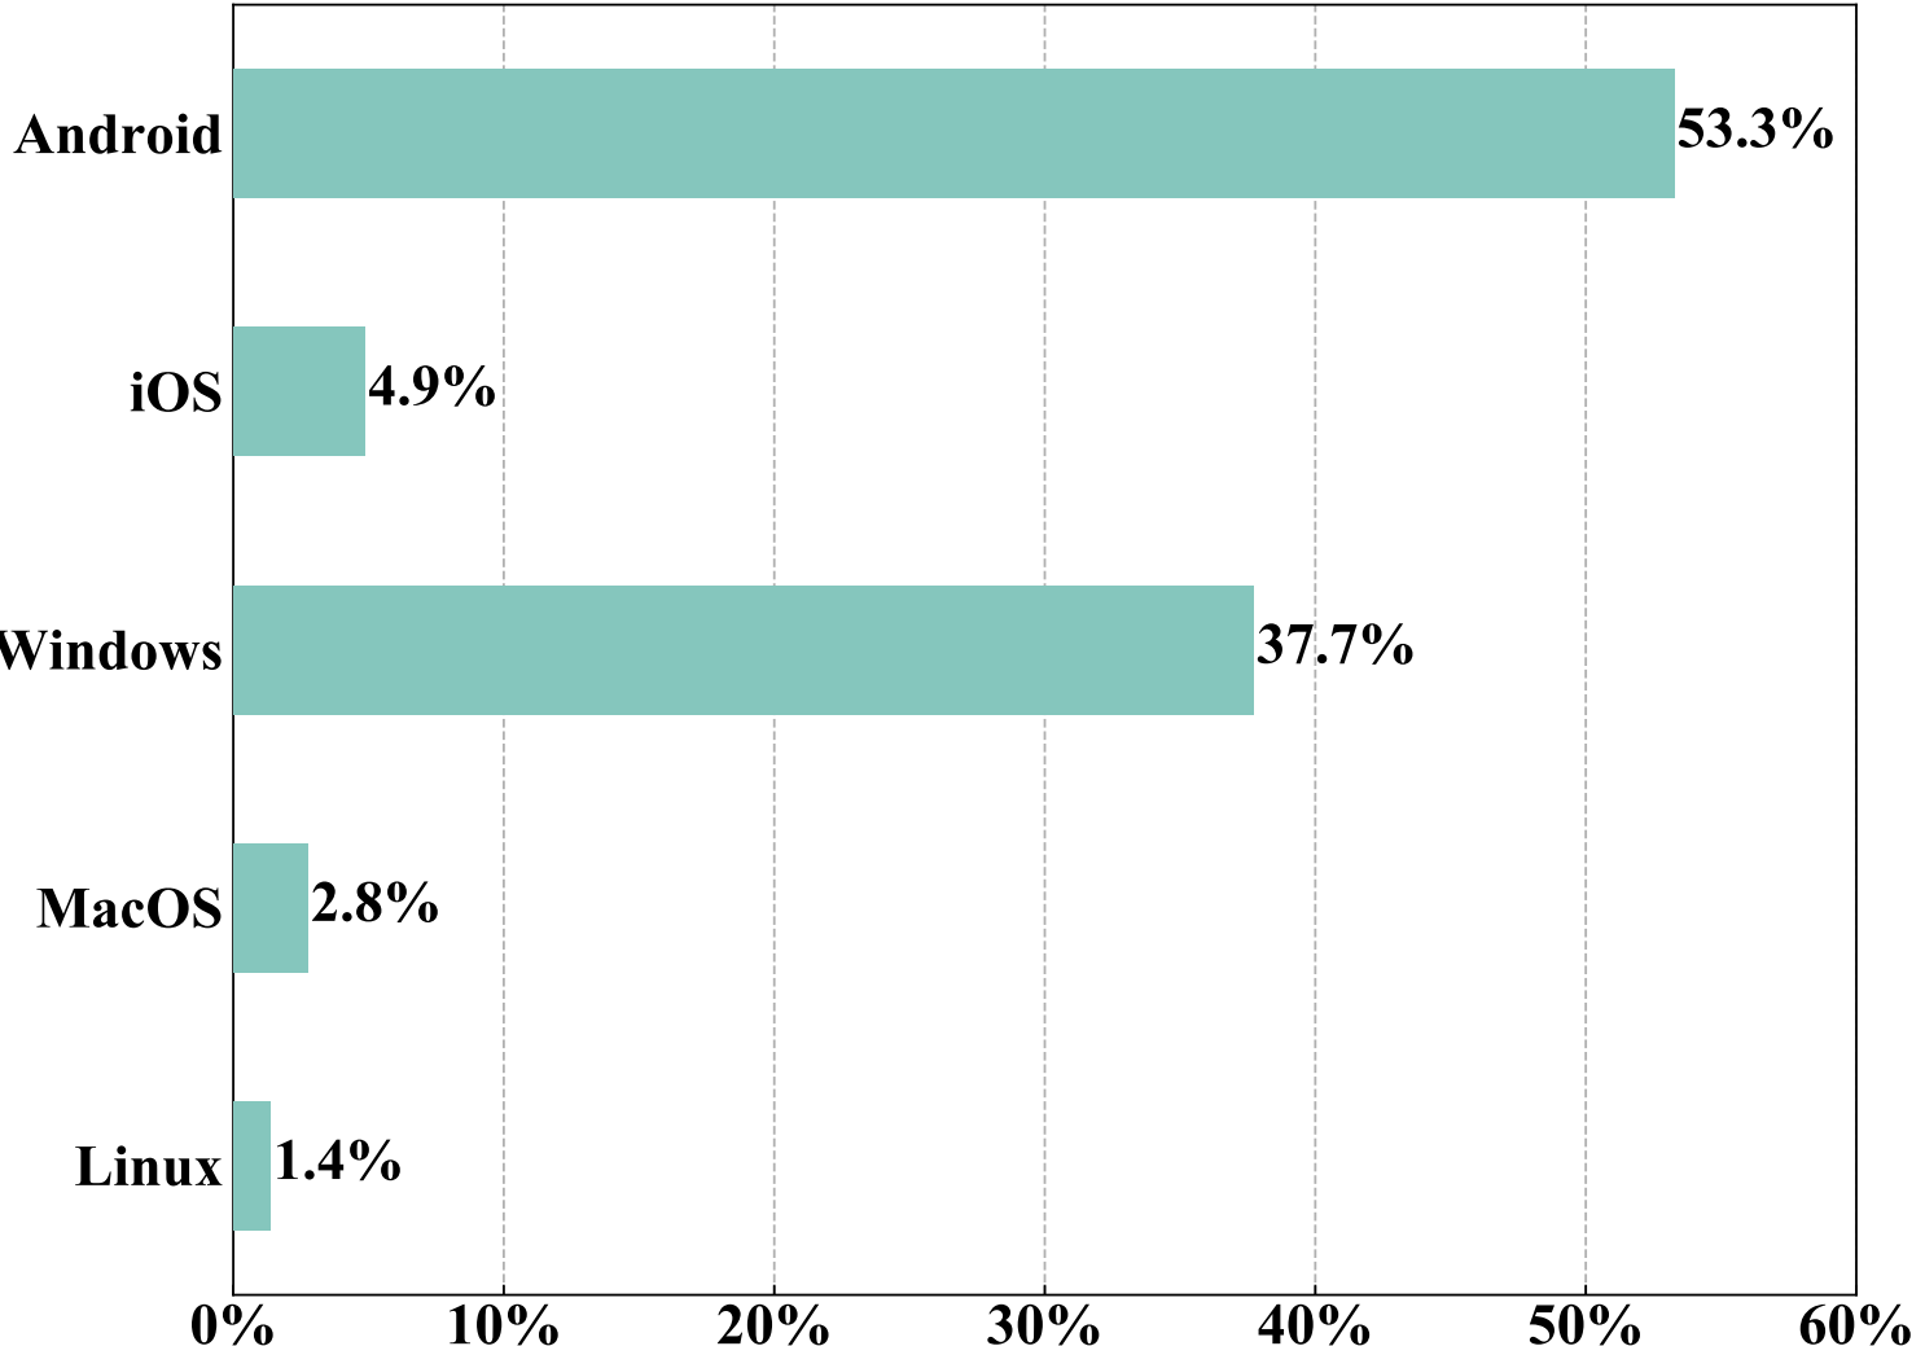
\includegraphics[width=\textwidth]{3-6-1}
      \caption{操作系统类型分布}
    \end{subfigure}%
    \hspace{10pt}
    \begin{subfigure}[b]{0.32\textwidth}
      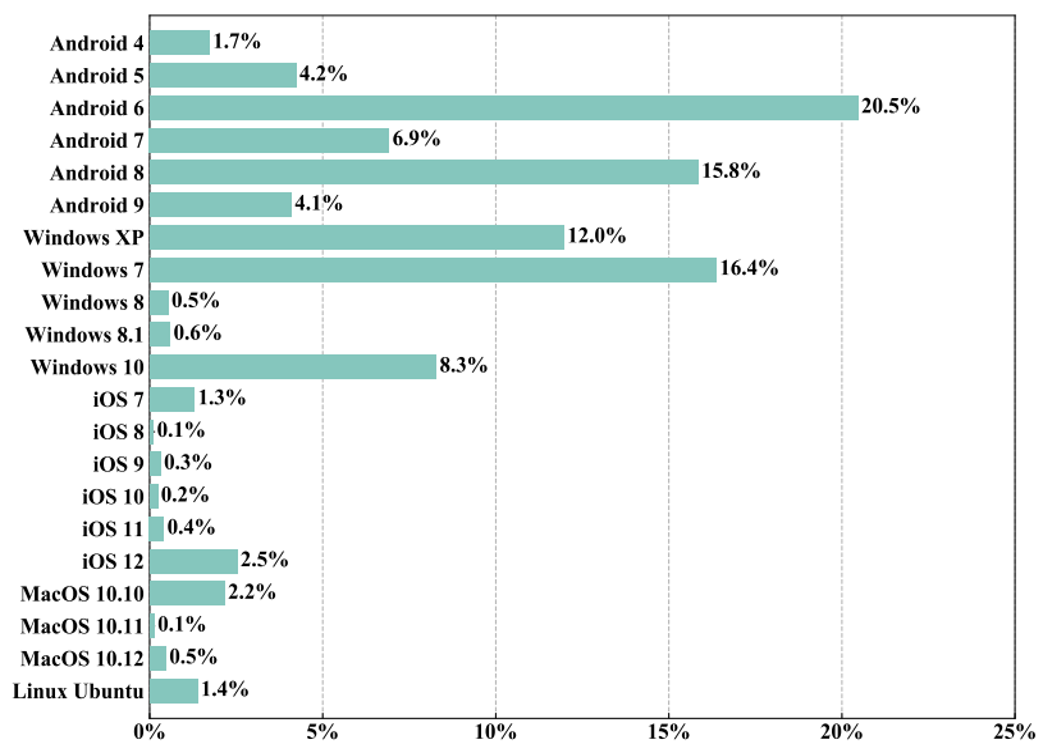
\includegraphics[width=\textwidth]{3-6-2}
      \caption{操作系统版本分布}
    \end{subfigure}
    \hspace{10pt}
    \begin{subfigure}[b]{0.29\textwidth}
      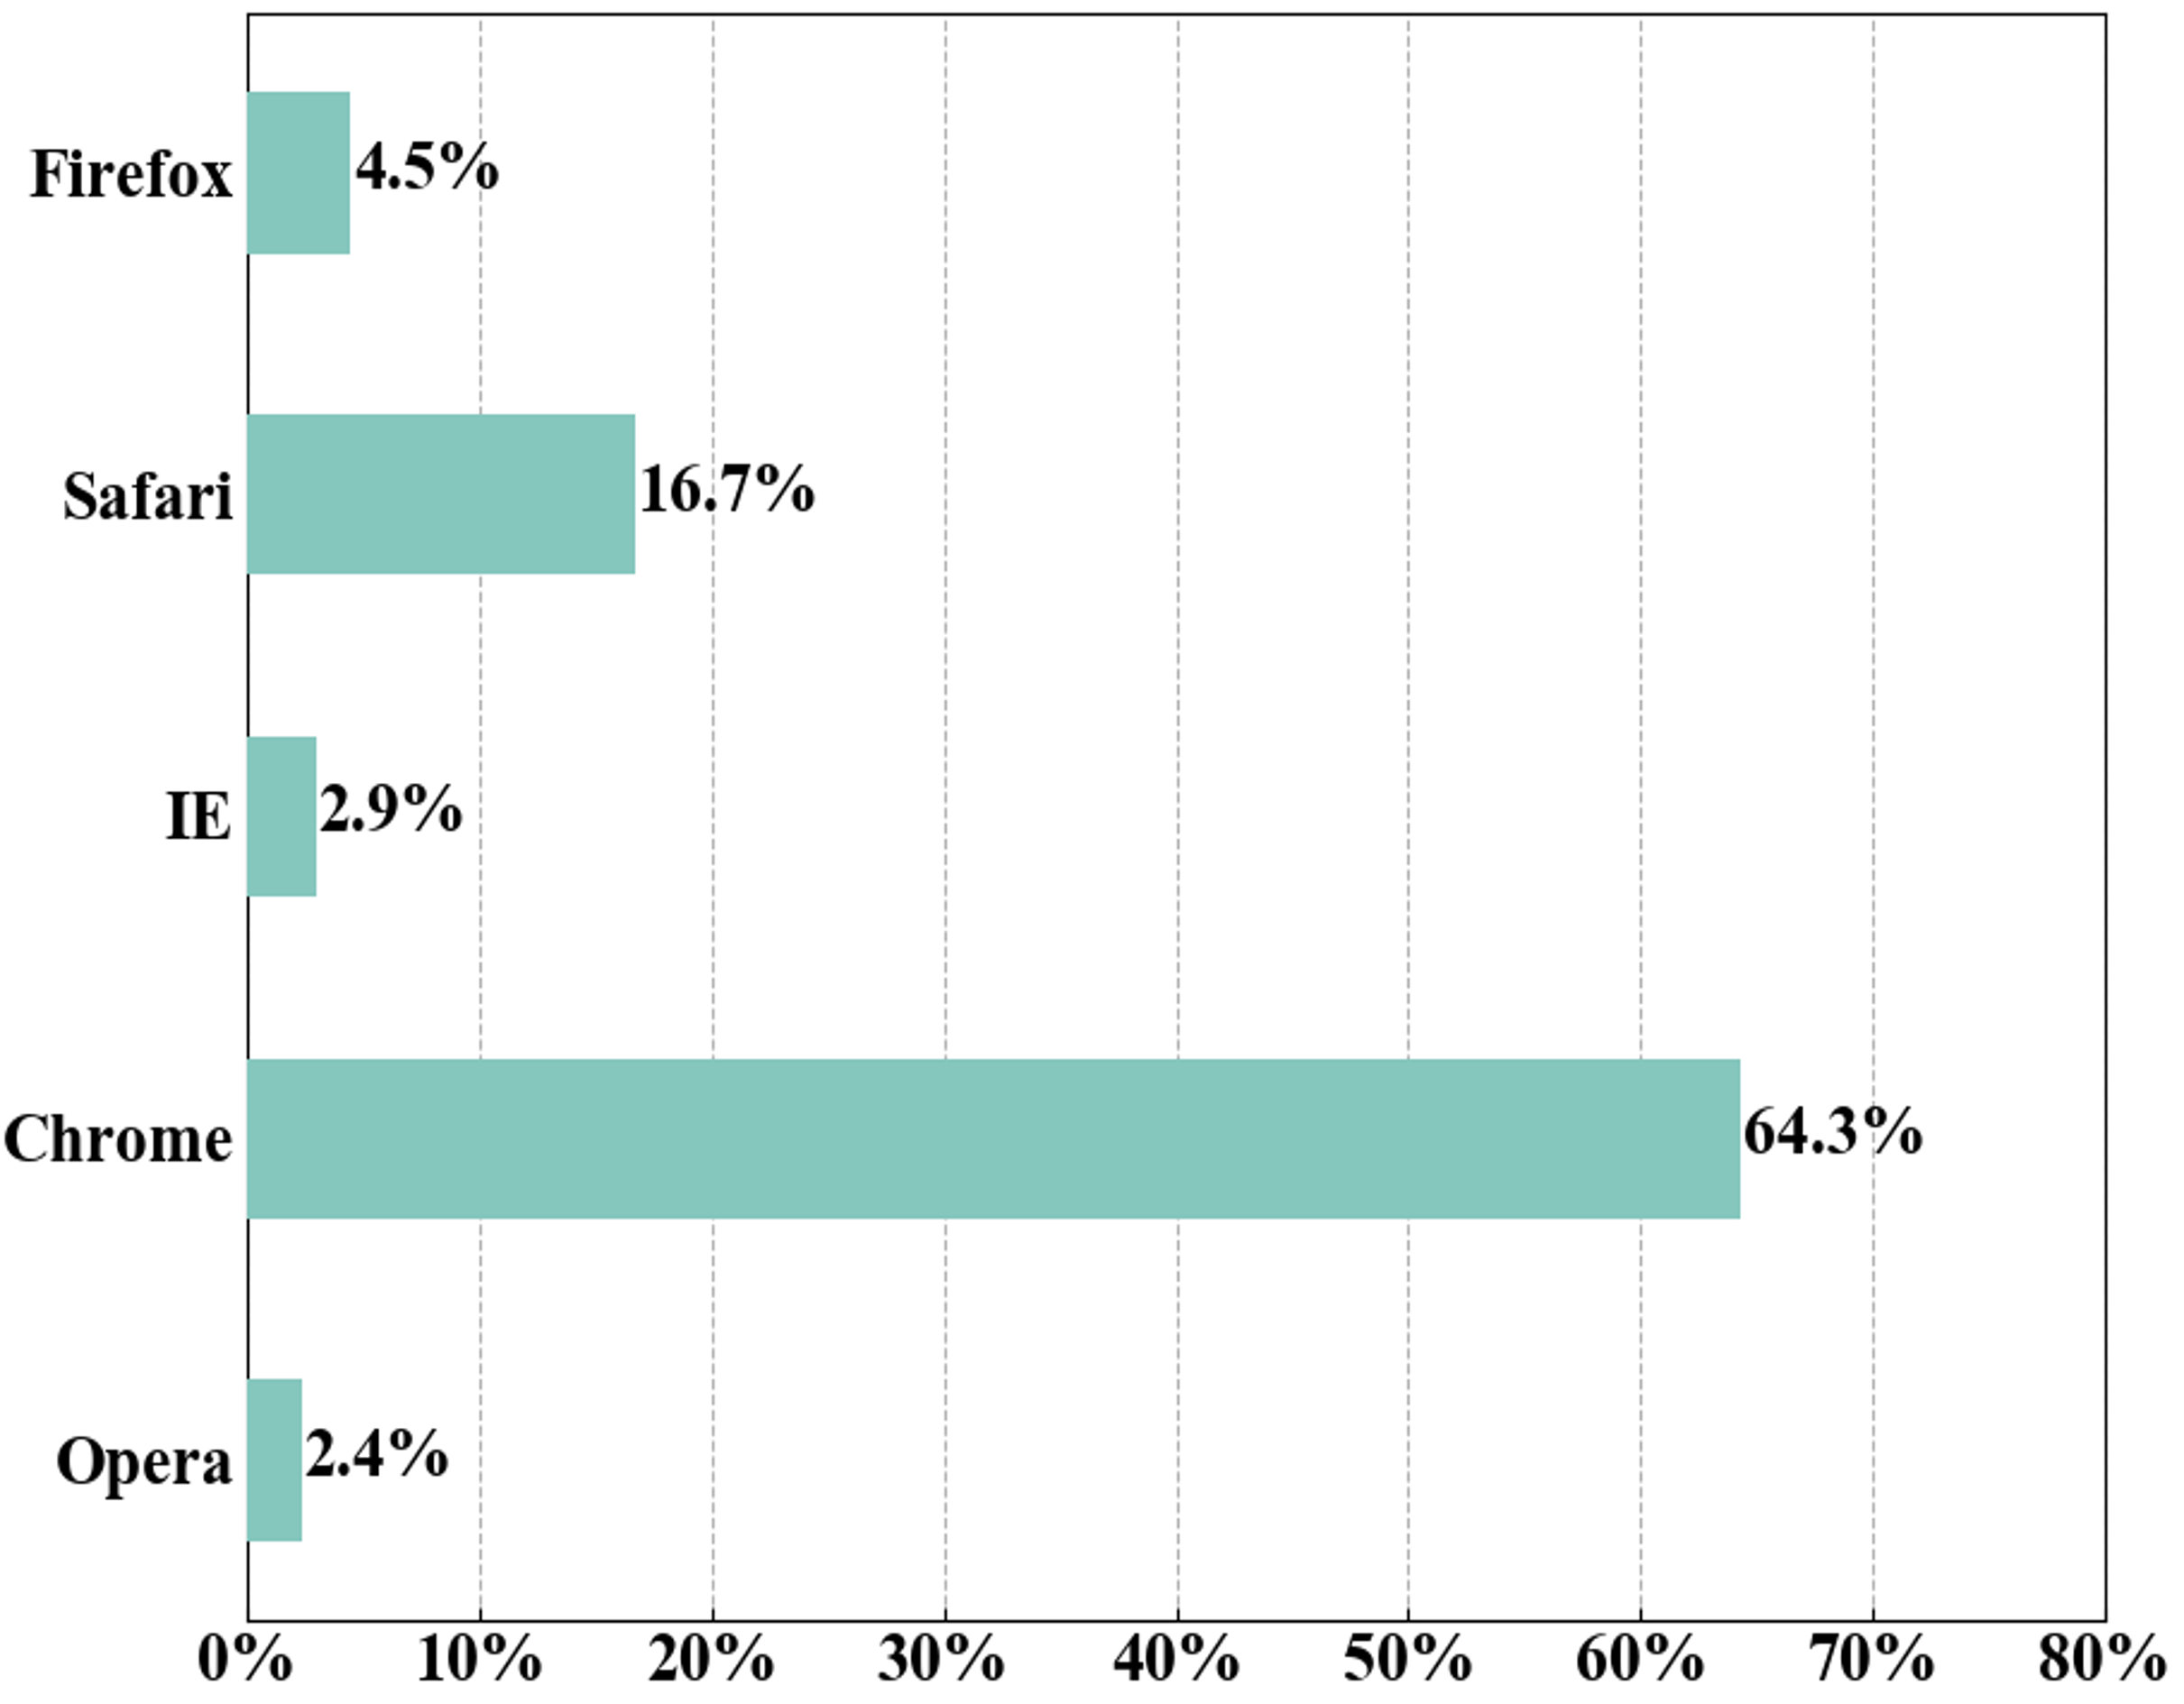
\includegraphics[width=\textwidth]{3-7}
      \caption{浏览器类型分布}
    \end{subfigure}  
    \centering  
    \bicaption{数据集中的主机属性分布(a)操作系统类型分布,(b)操作系统版本分布,(c)浏览器类型分布}{Distribution of host attributes in the dataset(a)Operating system type distribution, (b)Operating system version distribution, (c)Browser type distribution}
\end{figure}

\section{实验设计与结果分析}

\subsection{模型对比}

本节将分别测试3.3节中介绍的逻辑回归模型、最近邻居模型、随机森林模型、XGBoost模型以及LightGBM模型等五类机器学习模型在主机属性识别任务中的效果和性能。

若无特殊说明,本文所有实验都在同一环境中进行,以避免因机器性能不同带来的实验结果误差。实验环境的操作系统为Windows,CPU型号为Intel Core i7-7300HQ,GPU型号为GTX 1080Ti,内存大小为32GB,采用的编程语言为Python语言,调用的算法实现库为Sklearn库。

在对比实验中,本文采取的评估指标主要有准确率、精度、召回率、F1分数、PR曲线和模型预测速率。其中,F1分数是统计学中用来衡量分类模型精确度的一种指标。它同时兼顾了分类模型的准确率和召回率,可以看作是模型准确率和召回率的一种调和平均。

\begin{figure}[!h]
    \centering
    \begin{subfigure}[b]{0.8\textwidth}
      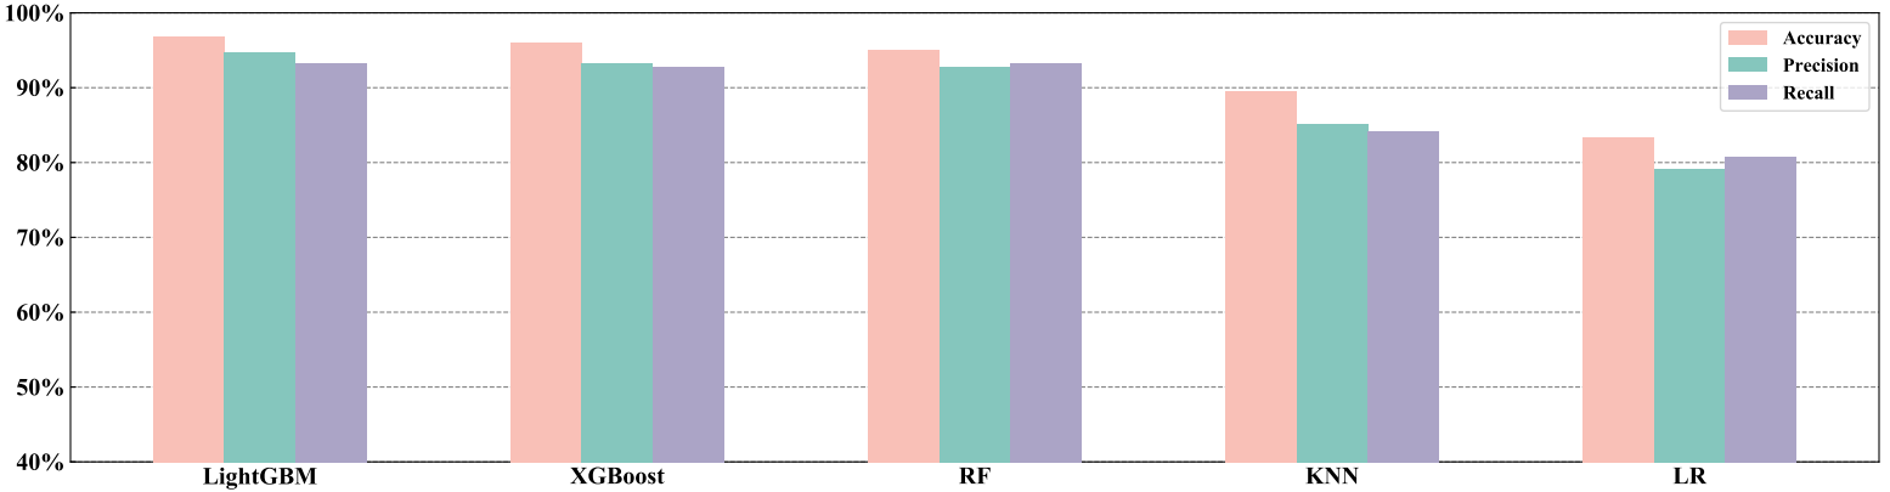
\includegraphics[width=\textwidth]{3-8-1}
      \caption{操作系统类型识别结果}
    \end{subfigure}
    \begin{subfigure}[b]{0.8\textwidth}
      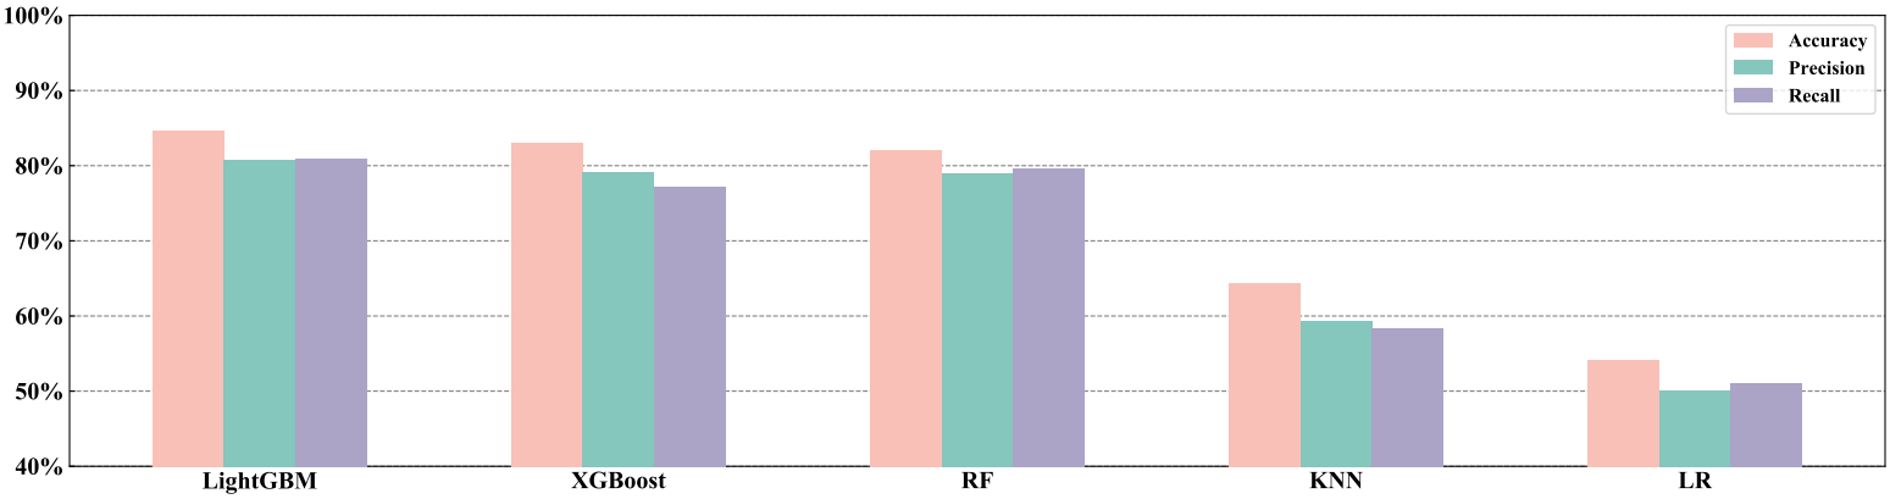
\includegraphics[width=\textwidth]{3-8-2}
      \caption{操作系统版本识别结果}
    \end{subfigure}
    \begin{subfigure}[b]{0.8\textwidth}
      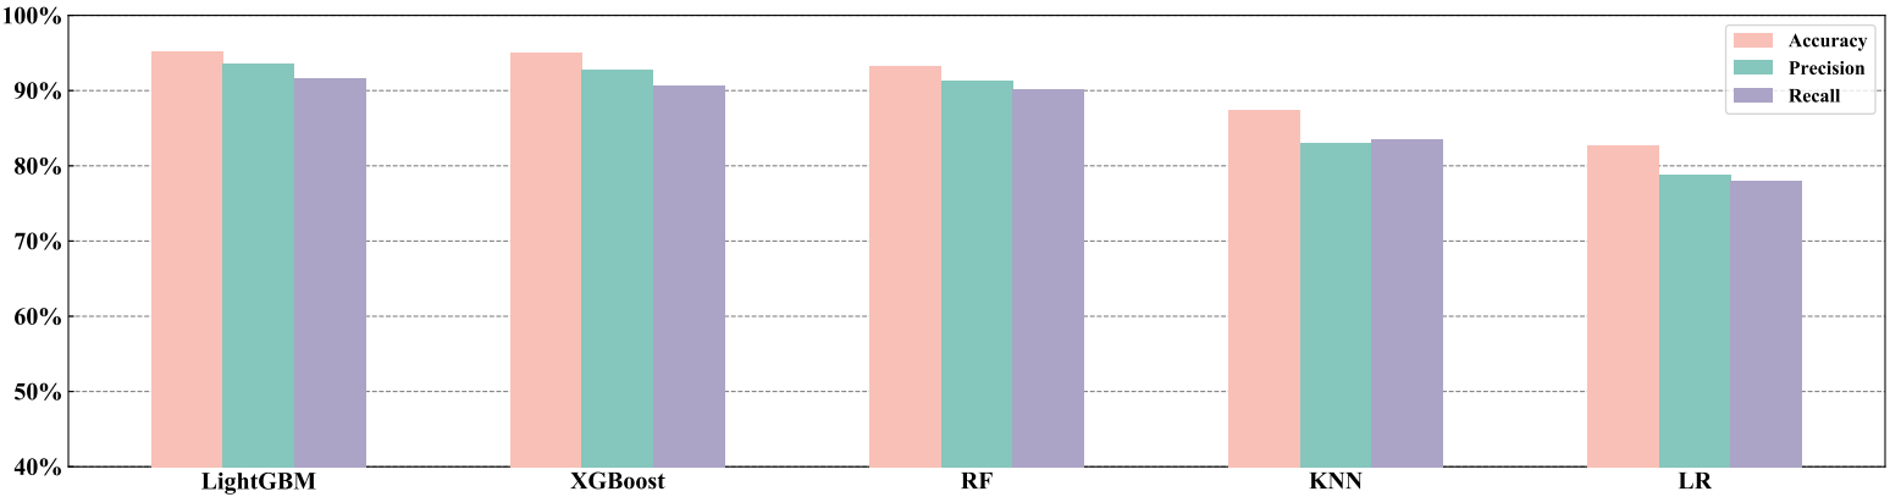
\includegraphics[width=\textwidth]{3-8-3}
      \caption{浏览器类型识别结果}
    \end{subfigure}
    \bicaption{识别任务准确率、精度以及召回率对比(a)操作系统类型识别结果,(b)操作系统版本识别结果,(c)浏览器类型识别结果}{Comparison of identification task accuracy, precision and recall(a)Operating system type identification results, (b)Operating system version identification results, (c)Browser type identification results}
    \label{fig:3-8}
\end{figure}

如图3.8所示,在准确率、精度以及召回率方面,LightGBM模型在所有识别任务中的表现均是最佳。在操作系统和浏览器的类型识别任务中,RF模型、XGBoost模型以及LightGBM模型的各项指标都在90\%以上,充分显示了集成树模型的优越性。在主机属性识别任务中,大部分输入特征均为类别特征,而树模型的分类策略对这种离散特征的适应性非常强,再经过集成模型对基学习器的效果改善,使得集成树模型较为适用于该识别任务。KNN模型和LR模型虽然三项指标都达到了80\%左右,但由于算法结构较为简单,更适合处理线性分类任务,在决策空间较为复杂的主机属性识别任务中效果较差。

\begin{figure}[!h]
    \centering
    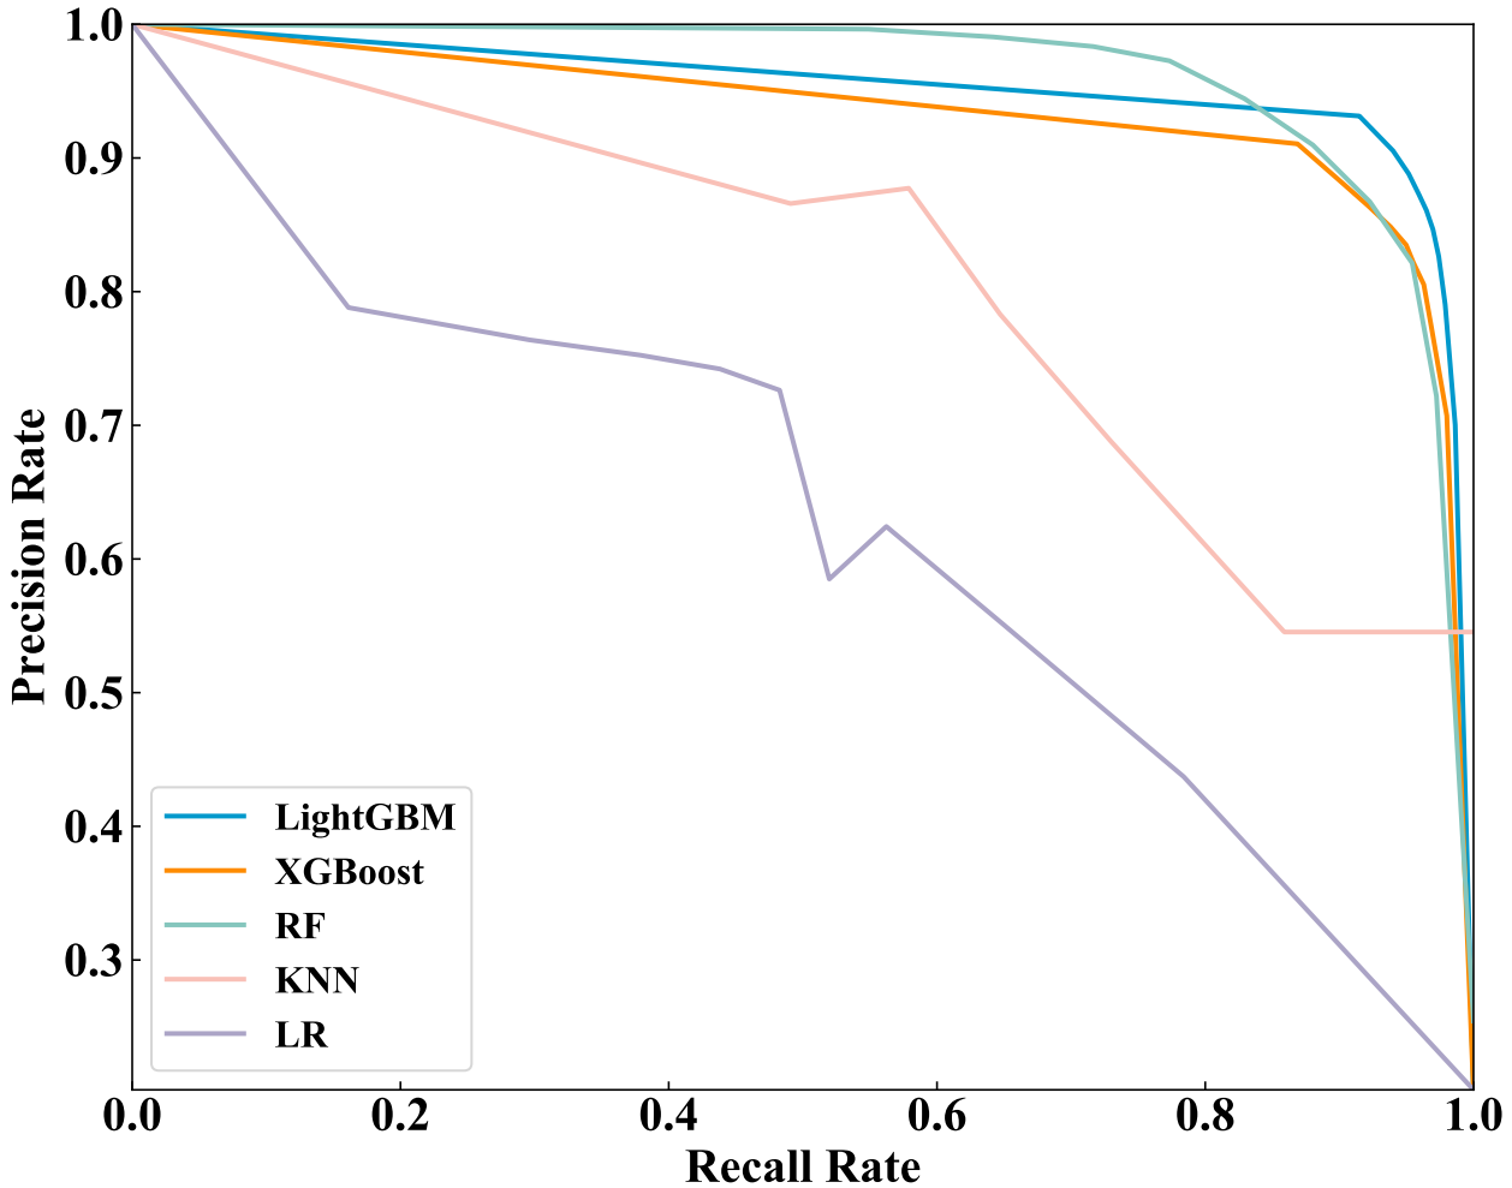
\includegraphics[width=0.6\textwidth]{3-9}
    \bicaption{操作系统版本识别任务PR曲线}{The PR curve of operating system version identification task}
    \label{fig:3-9}
\end{figure}

PR曲线是以召回率为横轴,以精度为纵轴绘制出的曲线,可以直观衡量一个模型的预测能力。在操作系统版本识别结果中,如图3.9所示,RF模型、XGBoost模型以及LightGBM模型的PR曲线均将KNN模型和LR模型的PR曲线完全包住,说明前三者的性能优于后者。而RF模型、XGBoost模型、LightGBM模型的PR曲线由于存在交叉点,不能根据以上标准分析优劣,但可以借助平衡点即召回率和精度相等的点比较性能。可以看到,LightGBM模型在平衡点处的值最大,说明该模型的性能更佳。

\begin{figure}[!h]
    \centering
    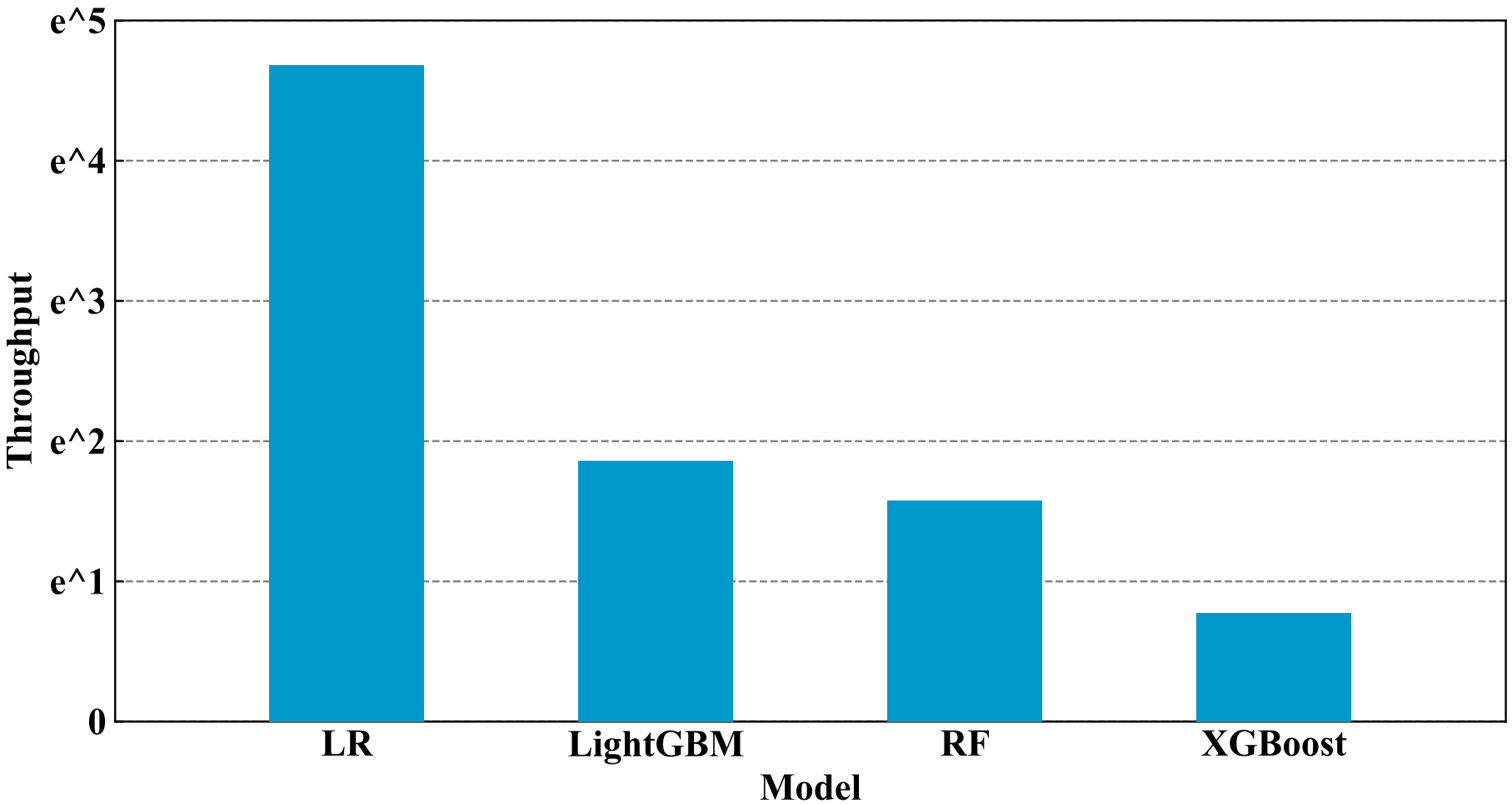
\includegraphics[width=0.8\textwidth]{3-10}
    \bicaption{操作系统版本识别任务吞吐量柱状图}{The throughput histogram of Operating system version identification task}
    \label{fig:3-10}
\end{figure}

通过分析在操作系统版本识别任务中的吞吐量可以得到各模型之间的预测速率差异。如图3.10所示,LR模型由于简单的分类策略,识别效率最高,比位于第二名的LightGBM模型快几十倍。在三类集成树模型中,LightGBM模型的预测速率最快,这主要是因为LightGBM模型采用直方图算法优化了树的生长速率,并对多线程任务进行了特殊优化,更适合多分类任务。对于KNN模型,由于独特的识别算法,其预测速率依赖于训练样本空间的规模,因此不适合在单一任务中与其他模型进行对比。

通过以上实验结果对比可以发现,LightGBM模型由于在GBDT算法的基础上进行了优化改进,在准确率、精度、召回率、PR曲线以及模型预测速率等方面的表现都较为优越。因此,本章采用LightGBM模型作为主机属性发现任务中的最终模型。

\subsection{泛化性能评估}

为了验证模型的泛化性能,本节将数据集按照日期进行切分,以前四天的数据作为训练集,最后一天的数据作为测试集,比较LightGBM模型在两个数据集上的性能差异。

图3.11展示了LightGBM模型在操作系统类型识别任务中的识别结果。从柱状图中可以看到,模型在训练集和测试集中的识别结果差异性非常小,准确率、精度以及召回率的最大差异不超过1\%。在折线图中,LightGBM模型识别每一类操作系统的精度和召回率变化同样较小。由此说明,基于协议字段特征和流统计特征的LightGBM模型具备很强的泛化能力。

\begin{figure}[!htbp]
    \centering
    \begin{subfigure}[b]{0.33\textwidth}
      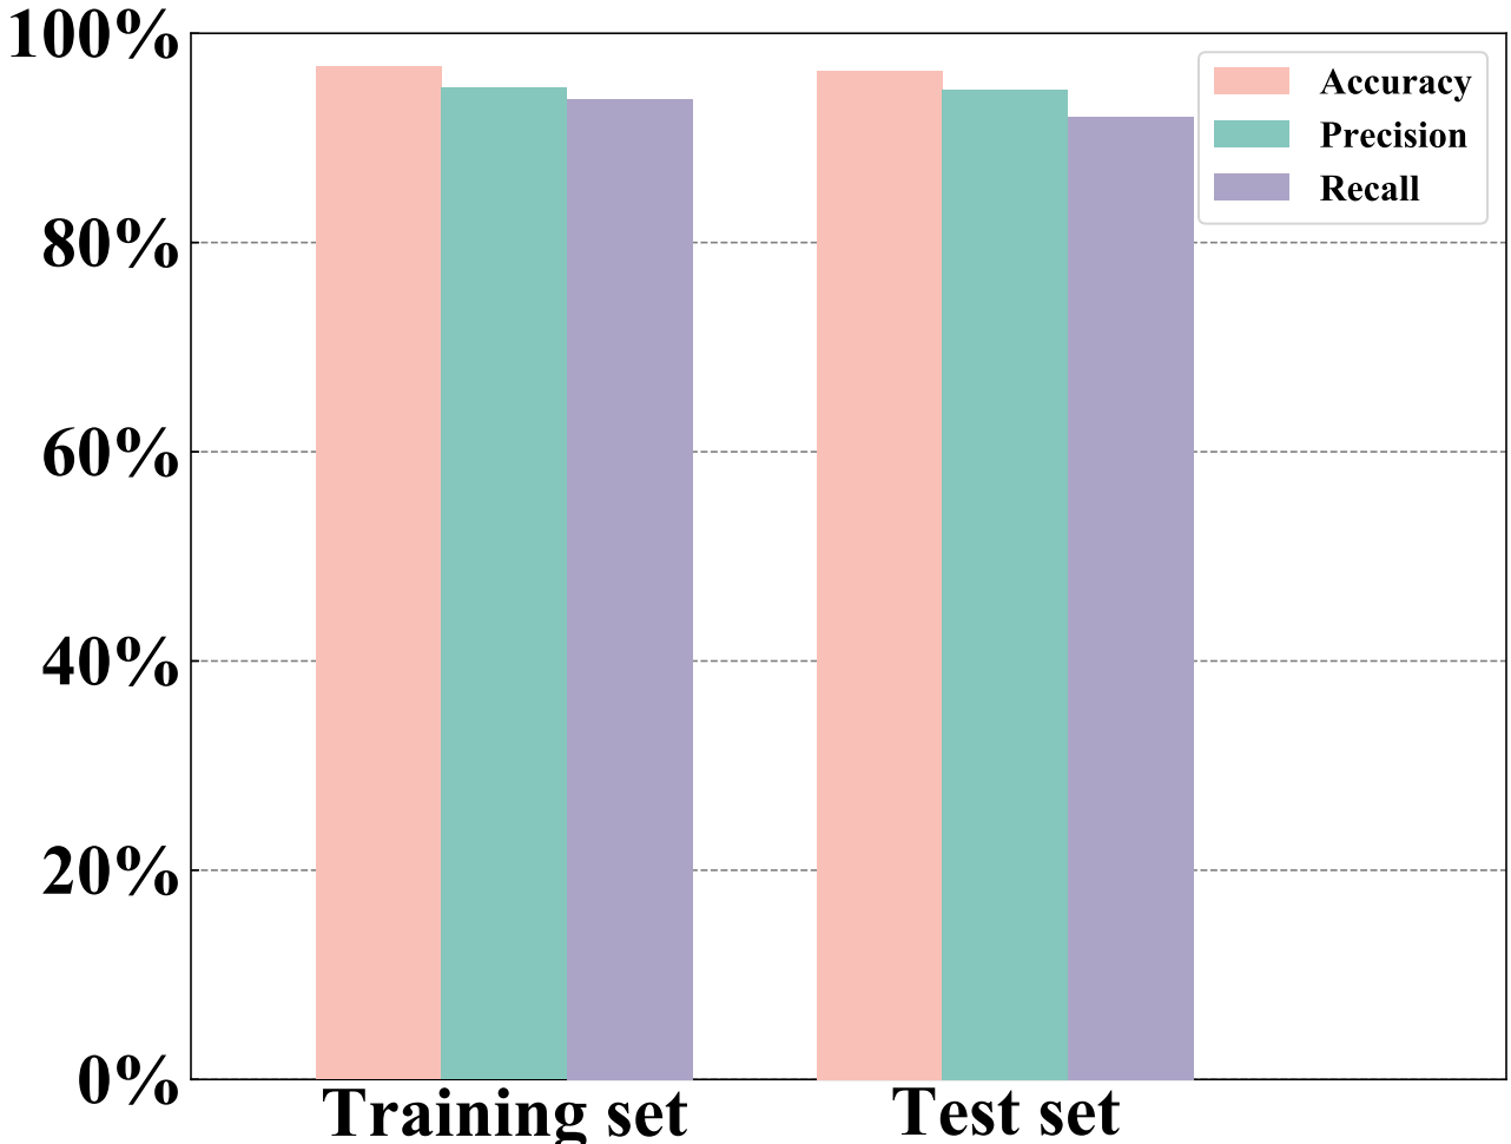
\includegraphics[width=\textwidth]{3-11-1}
      \caption{准确率、精度和召回率柱状图}
    \end{subfigure}%
    \hspace{20pt}
    \begin{subfigure}[b]{0.4\textwidth}
      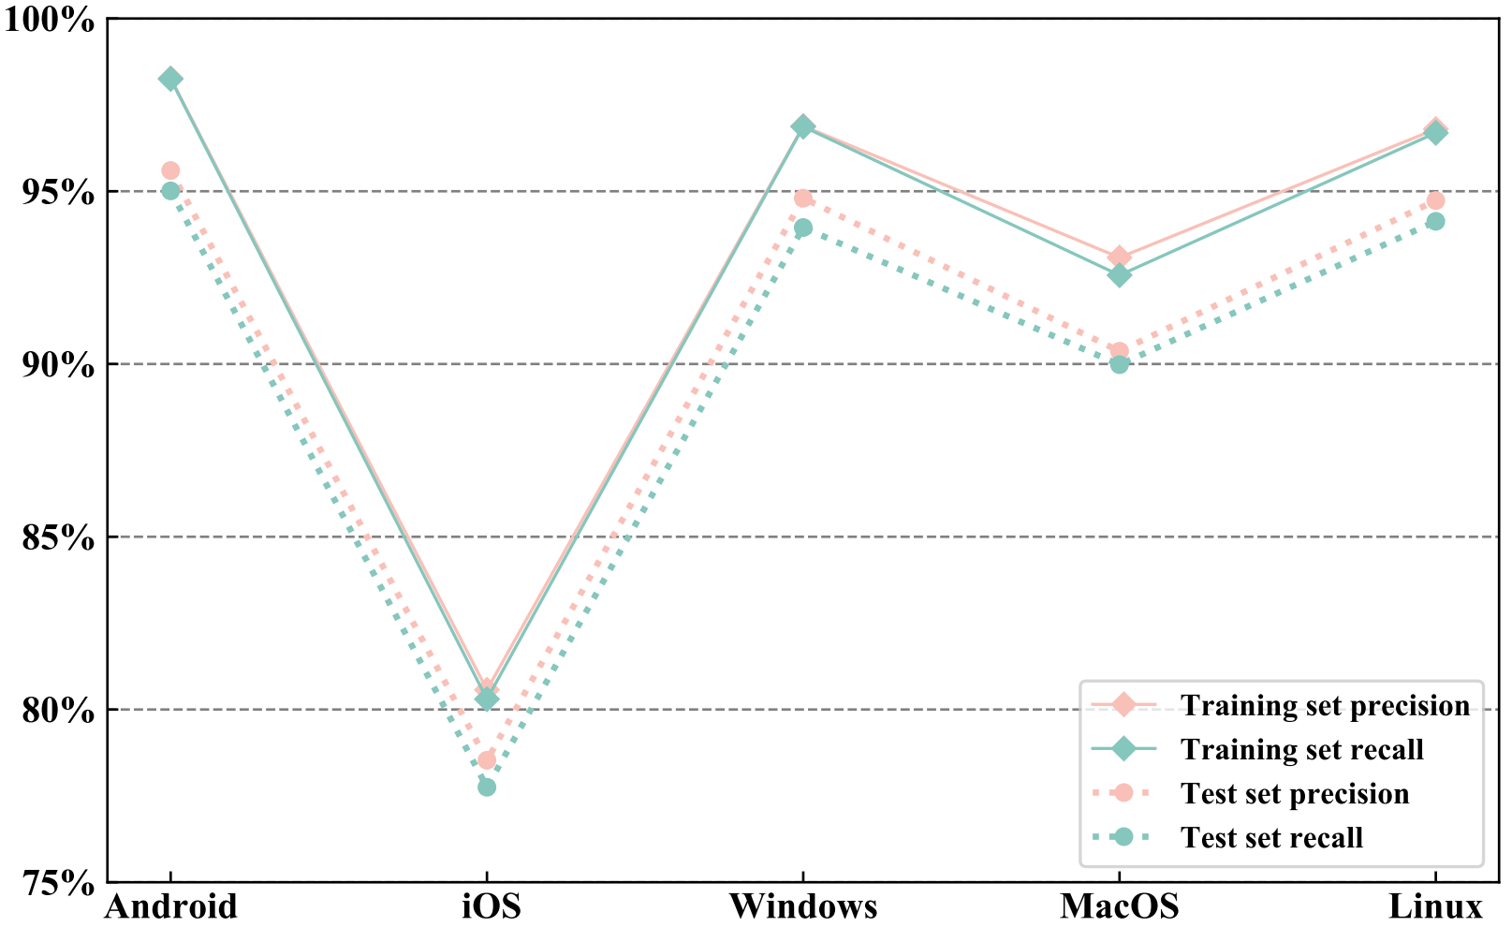
\includegraphics[width=\textwidth]{3-11-2}
      \caption{精度和召回率折线图}
    \end{subfigure}
    \bicaption{操作系统类型识别(a)准确率、精度和召回率柱状图,(b) 精度和召回率折线图}{Operating system type identification results(a)Histogram of accuracy, precision and recall, (b)Line chart of accuracy and recall}
    \label{fig:3-11}
\end{figure}

\subsection{主机属性识别结果}

通过以上实验对比,不难发现LightGBM模型在众多机器学习模型中拥有最优的表现。因此,本章基于13维协议字段特征和上百维流统计特征,结合LightGBM模型,提出了开放环境中的细粒度主机属性发现技术,可以高效、精准地识别加密网络中客户端主机的多维属性。利用该技术对数据集中的所有样本进行主机属性识别,可得结果如表3.7-3.9所示。

在操作系统类型识别任务中,分类器在测试集上的识别准确率达到了96.29\%,F1值也高达91.53\%。其中,Android系统的识别效果最好,精度为98.27\%,比平均值高了5\%左右,这主要是因为主机属性识别任务是一个类别不均衡任务,Android系统对应的样本量在数据集中最多,导致学习器在训练过程中对其有所偏好。Linux系统和Windows系统的识别效果次之,MacOS系统和iOS系统的识别效果最差,这是因为iOS系统和MacOS系统同属于一家厂商,其网络协议栈指纹的相似性较高,导致在识别过程中容易混淆。

\begin{table}[!h]
    \bicaption{操作系统类型识别结果}{Operating system type identification results}
    \centering
    \footnotesize
    \setlength{\tabcolsep}{8pt}
    \renewcommand{\arraystretch}{1}
\begin{tabular}{|c|c|c|c|c|c|c|c|}
\hline
\multirow{2}{*}{\textbf{ID}} & \multirow{2}{*}{\textbf{操作系统类型}} & \multicolumn{3}{c|}{\textbf{训练集}} & \multicolumn{3}{c|}{\textbf{测试集}} \\ \cline{3-8} 
 &  & \textbf{Precision} & \textbf{Recall} & \textbf{F1} & \textbf{Precision} & \textbf{Recall} & \textbf{F1}\\ \hline
1 & Android & 98.27\% & 95.60\% & 96.92\% & 98.25\% & 95.01\% & 96.60\% \\ \hline
2 & iOS & 80.57\% & 78.53\% & 79.54\% & 80.30\% & 77.75\% & 79.00\% \\ \hline
3 & Windows & 96.89\% & 94.80\% & 95.83\% & 96.87\% & 93.95\% & 95.39\% \\ \hline
4 & MacOS & 93.08\% & 90.37\% & 91.70\% & 92.57\% & 89.98\% & 91.26\% \\ \hline
5 & Linux & 96.80\% & 94.73\% & 95.75\% & 96.69\% & 94.13\% & 95.39\% \\ \hline
\multicolumn{2}{|c|}{\textbf{AVE}} & 93.12\% & 90.81\% & 91.95\% & 92.94\% & 90.16\% & 91.53\% \\ \hline
\multicolumn{2}{|c|}{\textbf{Accuracy}} & \multicolumn{3}{c|}{96.89\%} & \multicolumn{3}{c|}{96.29\%} \\ \hline
\end{tabular}
\end{table}

\begin{table}[!h]
    \bicaption{操作系统版本识别结果}{Operating system version identification results}
    \centering
    \footnotesize
    \setlength{\tabcolsep}{8pt}
    \renewcommand{\arraystretch}{1}
\begin{tabular}{|c|c|c|c|c|c|c|c|}
\hline
\multirow{2}{*}{\textbf{ID}} & \multirow{2}{*}{\textbf{操作系统版本}} & \multicolumn{2}{c|}{\textbf{测试集}} & \multirow{2}{*}{\textbf{ID}} & \multirow{2}{*}{\textbf{操作系统版本}} & \multicolumn{2}{c|}{\textbf{测试集}} \\ \cline{3-4} \cline{7-8}
 &  & \textbf{Precision} & \textbf{Recall} & & & \textbf{Precision} & \textbf{Recall} \\ \hline
1 & Android 4 & 81.23\% & 66.27\% & 12 & iOS 7 & 99.44\% & 99.36\% \\\hline
2 & Android 5 & 71.44\% & 60.67\% & 13 & iOS 8 & 70.58\% & 86.04\% \\\hline
3 & Android 6 & 94.64\% & 87.23\% & 14 & iOS 9 & 72.18\% & 80.84\% \\\hline
4 & Android 7 & 89.27\% & 59.85\% & 15 & iOS 10 & 51.45\% & 69.11\% \\\hline
5 & Android 8 & 67.07\% & 88.97\% & 16 & iOS 11 & 49.80\% & 69.10\% \\\hline
6 & Android 9 & 63.72\% & 42.41\% & 17 & iOS 12 & 57.36\% & 85.79\% \\\hline
7 & Windows XP & 98.30\% & 94.11\% & 18 & MacOS 10 & 99.26\% & 94.89\% \\\hline
8 & Windows 7 & 91.08\% & 95.07\% & 19 & MacOS 11 & 88.67\% & 66.50\% \\\hline
9 & Windows 8 & 78.87\% & 43.36\% & 20 & MacOS 12 & 81.45\% & 64.82\% \\\hline
10 & Windows 8.1 & 90.99\% & 57.74\% & 21 & Ubuntu & 94.44\% & 95.38\% \\\hline
11 & Windows 10 & 89.19\% & 88.22\% & \multicolumn{2}{c|}{\textbf{AVE}} & 80.02\% & 75.99\% \\\hline
\end{tabular}
\end{table}

操作系统版本识别任务属于细粒度主机属性识别任务,在表3.8所示的实验结果中,可以看到细粒度主机属性的识别效果有所降低,平均的识别精度和召回率分别未80.02\%和75.99\%。通过观察识别结果的混淆矩阵,如图3.12所示,可以发现许多相邻版本的操作系统相互之间很容易产生识别混淆,这主要是因为部分操作系统在版本更新时,对网络协议栈的具体实现改动不多,导致其流量特征的可区分性不足,从而降低了分类器的识别准确性。


\begin{figure}[!h]
    \centering
    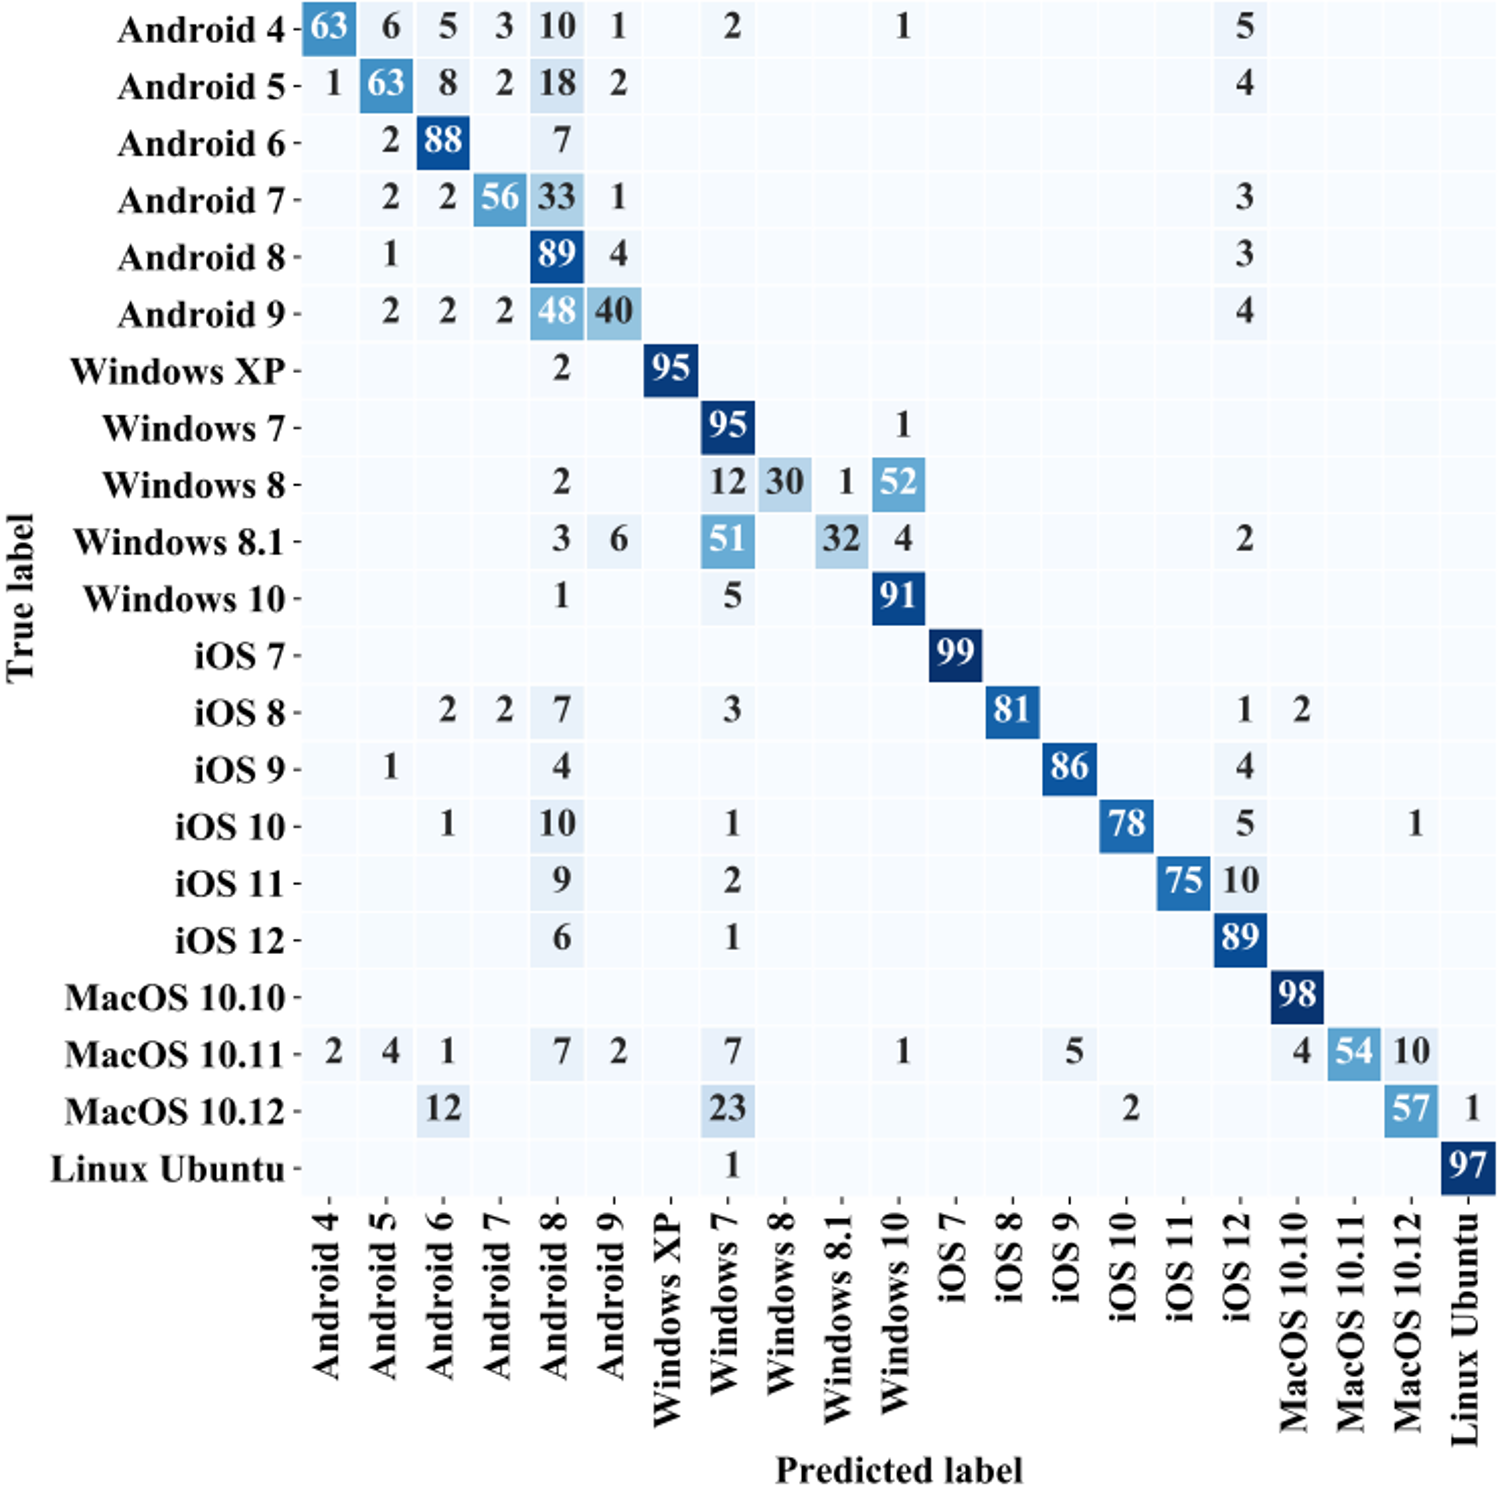
\includegraphics[width=0.7\textwidth]{3-12}
    \bicaption{操作系统版本识别任务混淆矩阵}{The confusion matrix of operating system version identification task}
    \label{fig:3-12}
\end{figure}

\vbox{}
在浏览器类型识别任务中,测试集的识别准确率和F1值分别为94.02\%和91.50\%,识别效果较好。其中,由于Firefox浏览器的TCP/IP协议栈指纹变化较少,拥有最佳的识别效果,而Chrome浏览器和Safari浏览器因为多平台支持和较频繁的版本更新,识别效果偏差。

\begin{table}[!htbp]
    \bicaption{浏览器类型识别结果}{Browser type identification results}
    \centering
    \footnotesize
    \setlength{\tabcolsep}{8pt}
    \renewcommand{\arraystretch}{1}
\begin{tabular}{|c|c|c|c|c|c|c|c|}
\hline
\multirow{2}{*}{ \textbf{ID}} & \multirow{2}{*}{ \textbf{浏览器类型}} & \multicolumn{3}{c|}{ \textbf{训练集}} & \multicolumn{3}{c|}{ \textbf{测试集}} \\ \cline{3-8} 
 &  &  \textbf{Precision} &  \textbf{Recall} &  \textbf{F1} & \textbf{Precision} &  \textbf{Recall} &  \textbf{F1} \\ \hline
1 & Firefox & 96.22\% & 93.31\% & 94.74\% & 94.09\% & 93.03\% & 93.56\%\\ \hline
2 & Safari & 90.25\% & 90.15\% & 90.20\% & 89.63\% & 89.17\% & 89.40\%\\ \hline
3 & IE & 94.45\% & 92.77\% & 93.60\% & 94.23\% & 91.47\% & 92.83\% \\ \hline
4 & Chrome & 90.37\% & 87.57\% & 88.95\% & 89.76\% & 87.60\% & 88.67\%\\ \hline
5 & Opera & 94.31\% & 92.55\% & 93.42\% & 94.44\% & 91.73\% & 93.07\%\\ \hline
\multicolumn{2}{|c|}{\textbf{AVE}} & 93.12\% & 91.27\% & 92.18\% & 92.43\% & 90.60\% & 91.50\%\\ \hline
\multicolumn{2}{|c|}{\textbf{Accuracy}} & \multicolumn{3}{c|}{94.89\%} & \multicolumn{3}{c|}{94.02\%} \\ \hline
\end{tabular}
\end{table}


\section{本章小结}

本章介绍了一种可在开放环境中识别细粒度主机属性的技术方法。该方法基于加密流量中的TLS会话数据,以双向网络流为单位,提取TCP/IP协议栈指纹,包括IP层的跳数、包长、分片标识等字段,TCP层的传输窗口大小、窗口缩放因子、最大报文长度等字段以及TLS层的版本、扩展长度、密钥算法套件序列等字段,再结合对应流的包长序列、时间序列和速率等统计特征,并将训练后的LightGBM模型作为分类器,可以从加密网络中被动识别主机的操作系统类型、版本和浏览器类型等主机属性。实验结果表明,本方法拥有较高的识别准确率、召回率和计算效率,并且泛化性能同样十分优秀。

\chapter{基于加密流原始载荷的主机属性发现}

前一章是基于TCP/IP协议栈指纹识别细粒度主机属性地研究,虽然识别效果较好,但这种方法对于特征的提取与构造比较依赖于丰富的网络流量分析经验,导致人工成本和时间成本较高。本章提出了一种基于深度学习模型的主机属性识别技术,利用表示学习的思想,不需要借助任何专家知识,只需将网络流的原始流数据作为分类器输入,便可完成细粒度的主机属性发现,并拥有更佳的识别效果。本章首先从该方法的背景意义和技术路线开始介绍,然后从可视化角度分析原始流信息的特征规律,接着通过分组实验对比不同深度学习模型的适用性,最后分析该方法的实验结果。

\section{引言}

由于近些年来计算性能和数据规模的发展,深度学习模型再度兴起,在信息时代的多个领域都有着重要应用。本章将神经网络模型引入主机属性发现技术中,利用表示学习思想自动挖掘加密流量指纹,用于细粒度主机属性的识别。

如图4.1所示,本方法首先从TLS加密会话中提取TCP SYN包和TLS Clinet Hello包的原始流信息,在经过归一化处理和平整对齐后,传入训练后的深度人工神经网络模型,即可得到客户端主机的多维主机属性。

\begin{figure}[!htbp]
    \centering
    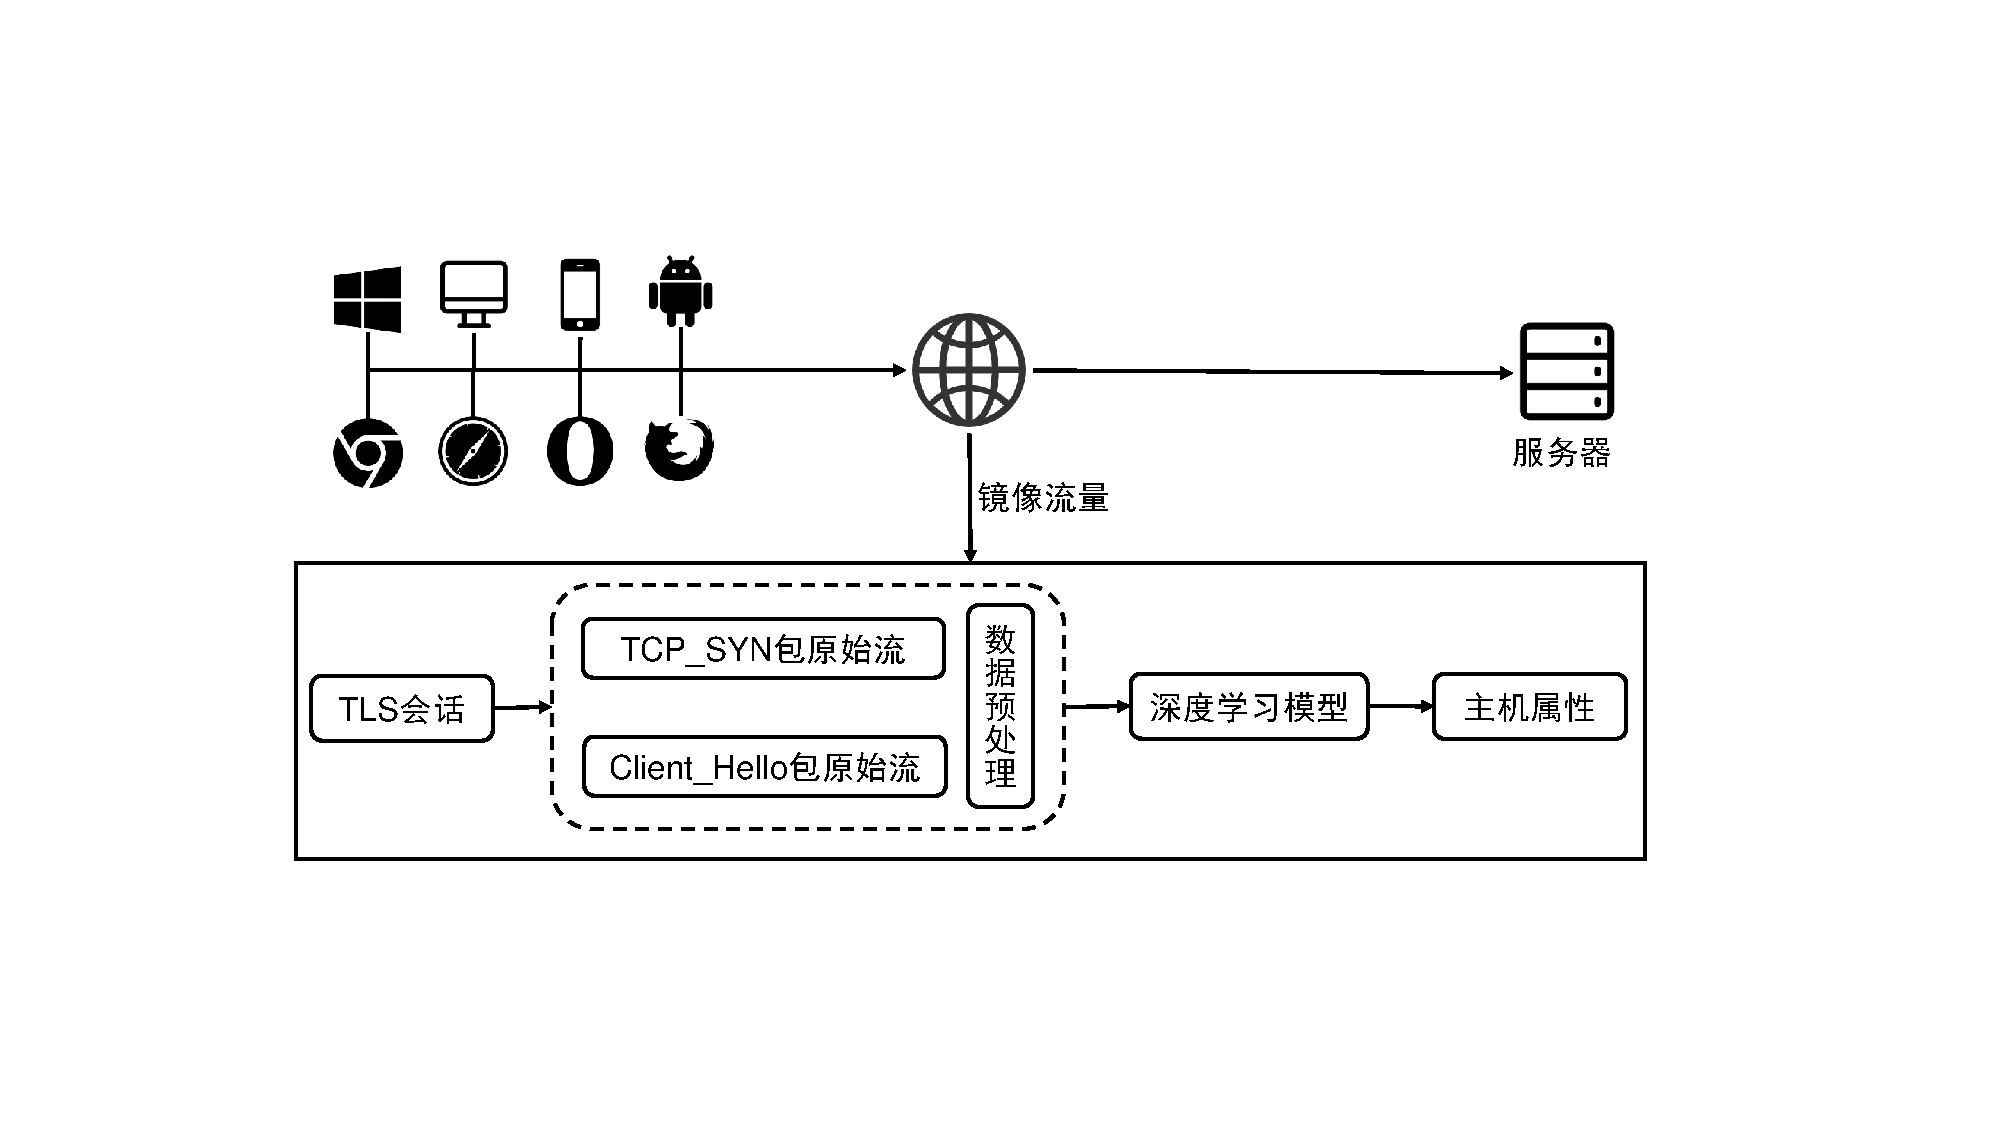
\includegraphics[width=0.9\textwidth]{研究点2结构}
    \bicaption{基于加密流原始载荷的主机属性发现}{Host attribute discovery based on encrypted stream original payload}
    \label{fig:4-1}
\end{figure}

\section{深度模型适应性分析}

在计算机视觉和自然语言处理等领域,最广为应用的模型是卷积神经网络(Convolutional Neural Networks, CNN)模型和循环神经网络(Recurrent Neural Network, RNN)模型。CNN模型可以自动挖掘数据中的序列信息和局部特征,拥有非常优越的性能。而在加密会话中,多数协议首部并未加密,将协议首部以字节序进行解析,可以发现其存在较为明显的局部特征,适合用CNN模型进行数据挖掘。而RNN模型是一类具有短期记忆能力的神经网络模型,同样适合处理网络流量这种序列数据。

\subsection{原始流量可视化分析}

在第三章中已经介绍过,传统的TCP/IP协议栈指纹一般都提取自TCP SYN包和TLS Client Hello包。而在一般的TLS会话过程中,被加密的部分通常是应用层载荷数据,由于考虑到通信的效率和稳定性,TCP SYN包和TLS Client Hello包中的数据都是明文信息。

\begin{figure}[!htbp]
    \centering
    \begin{subfigure}[b]{0.3\textwidth}
      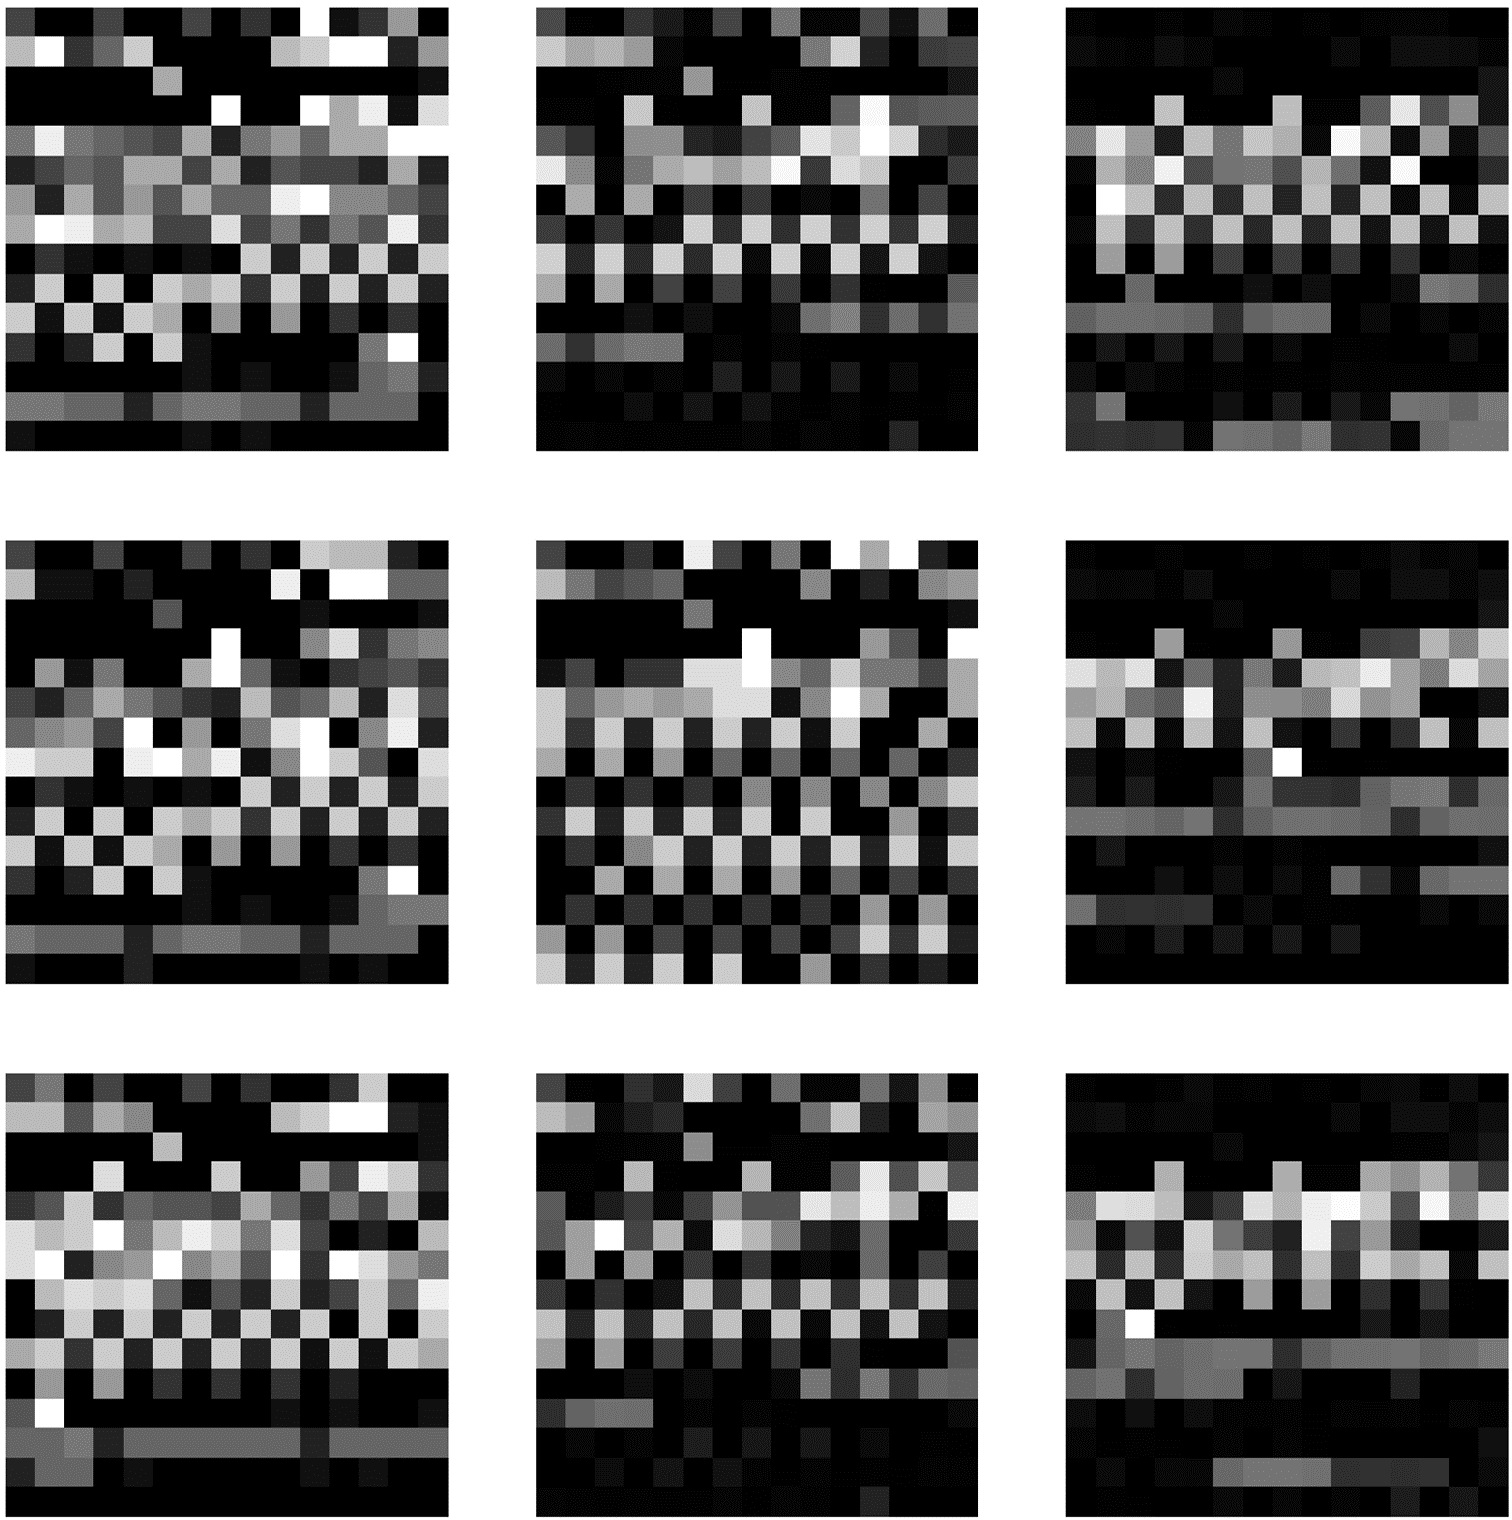
\includegraphics[width=\textwidth]{4-2-1}
      \caption{iOS系统}
    \end{subfigure}%
    \hspace{20pt}
    \begin{subfigure}[b]{0.3\textwidth}
      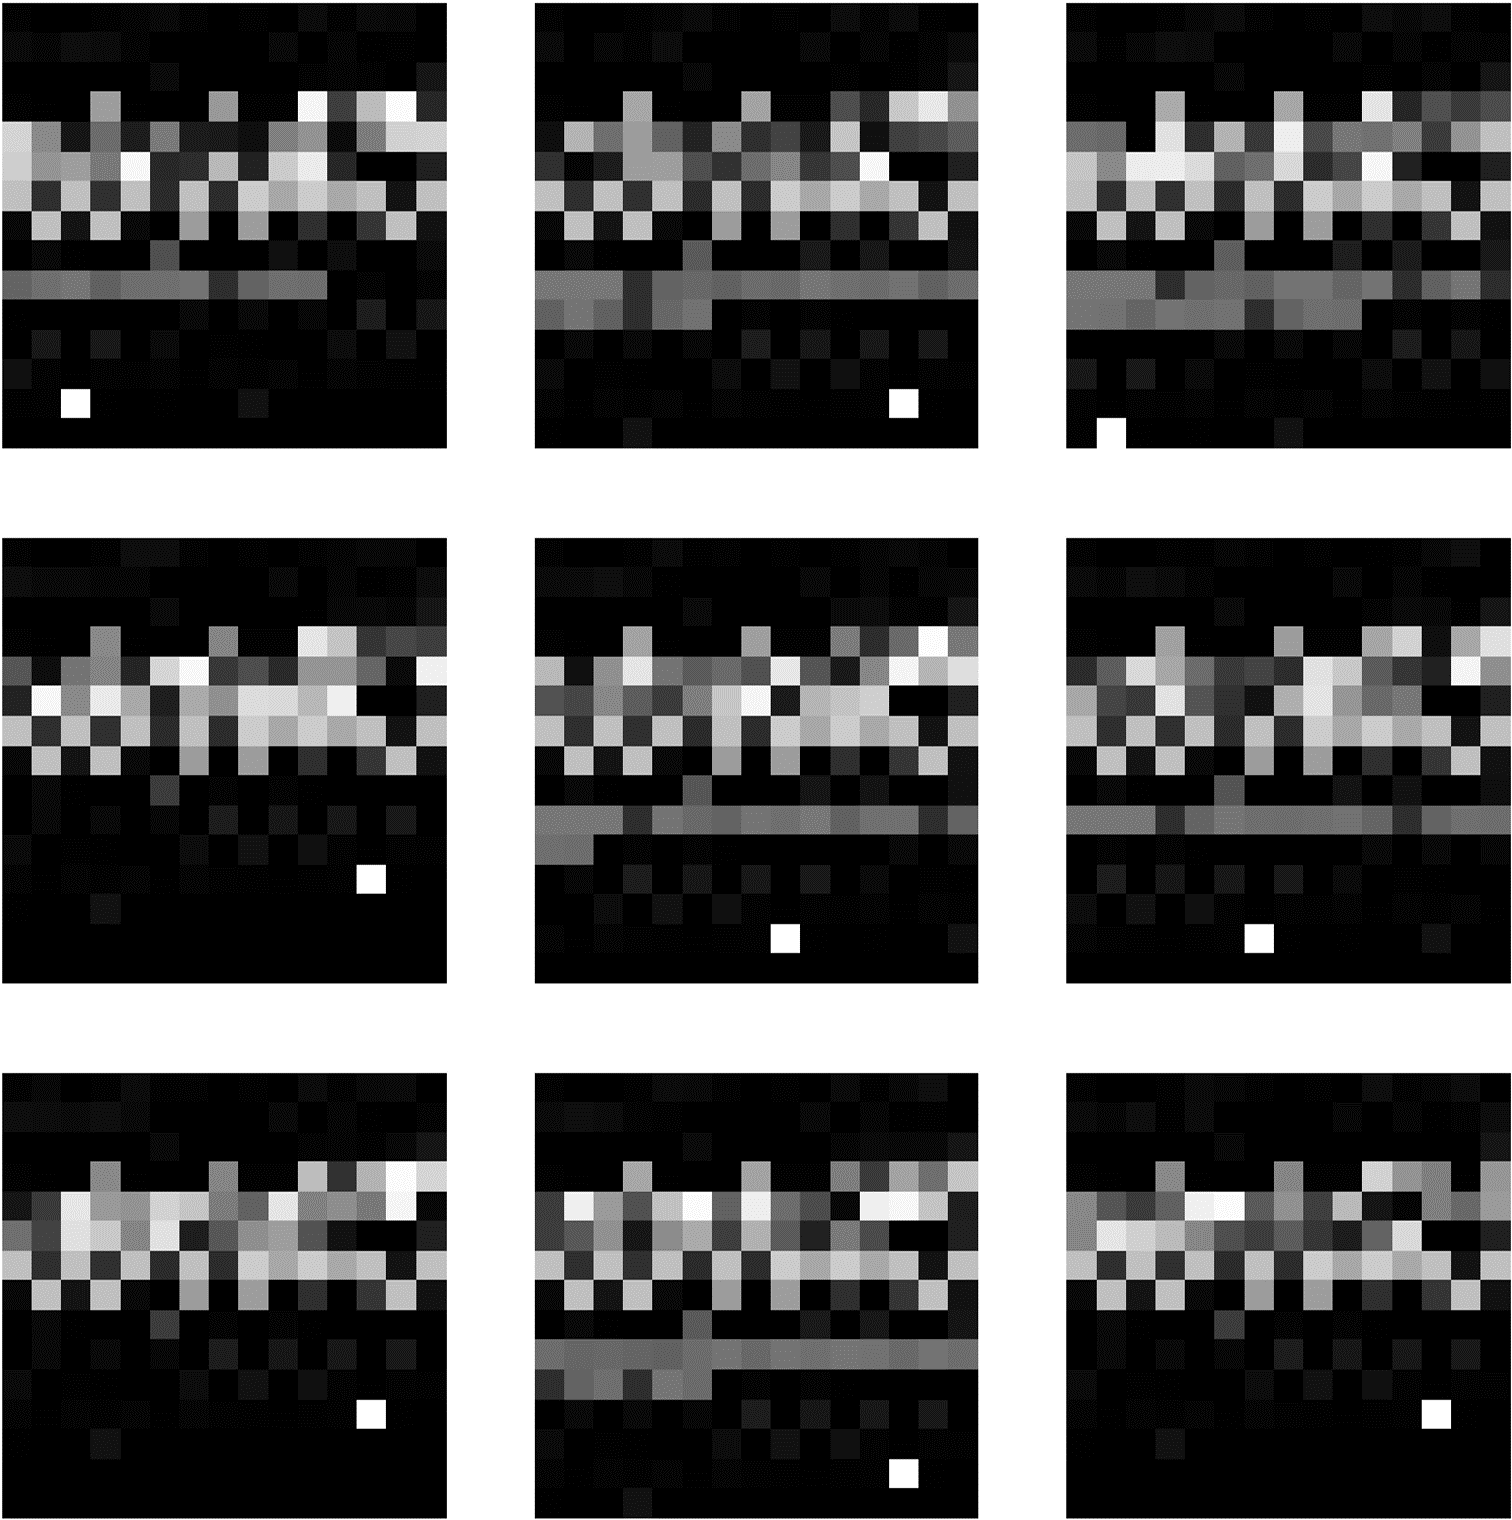
\includegraphics[width=\textwidth]{4-2-2}
      \caption{Linux系统}
    \end{subfigure}
    \bicaption{原始流量灰度图(a)iOS系统,(b)Linux系统}{Gray scale image of raw traffic(a)iOS system, (b)Linux system}
    \label{fig:3-6}
\end{figure}

在控制报文中,可以表达语义信息的最小单位一般是字节(byte),对应的数值为0-255。将TCP SYN包和TLS Client Hello包中的数据拼接后,并绘制256级灰度图,如图4.2所示,分别是由iOS系统和Linux系统产生的九条原始流对应的灰度图。在图a中,可以看到iOS系统发送的多数Client Hello握手报文中都存在高频的大小值交错序列片段,这一现象在其他操作系统的原始流灰度图中是看不到的。在图b中,由Linux系统产生的流量灰度图同样存在可被观察到的一些特征。例如,Client Hello握手报文中的有语义信息主要存在于报文的中上部,并且所有包都在尾部拥有一个独立亮点,其对应数值0xff01,在RFC文档中,该亮点表示TLS协议的重协商信息扩展。

通过对不同操作系统的原始流量可视化分析,可以发现不同属性的主机产生的流量存在显著的局部特征。又因网络流量数据本身所具备的顺序特性,使得主机属性发现技术中的TCP/IP协议栈指纹比较适合利用表征学习算法进行自动挖掘。

\subsection{基于深度前馈神经网络的原始载荷特征挖掘模型}

前馈神经网络是最早发明的简单人工神经网络。在前馈神经网络中,各神经元分别属于不同的层。每一层的神经元可以接收前一层神经元的信号,并产生信号输出到下一层。第一层叫输入层,最后一层叫输出层,其它中间层叫做隐藏层。整个网络中无反馈,信号从输入层向输出层单向传播,可用一个有向无环图表示。前馈神经网络具有很强的拟合能力,常见的连续非线性函数都可以用前馈神经网络来近似。

然而,传统的浅层学习方法受限于小规模的样本和低性能的计算单元,对复杂函数的表示能力有限。深度前馈神经网络(Deep Neural Networks, DNN)通过构建一种深层次的非线性网络结构,从海量训练数据中学习更有用的特征,可以实现复杂函数逼近,展现出了强大的表示学习能力。图4.3给出了只采用全连接层的DNN模型实例。本章构建的DNN网络模型采取5层全连接层作为隐藏层,并将Softmax层作为输出层,如表4.1所示。

\begin{figure}[!htbp]
    \centering
    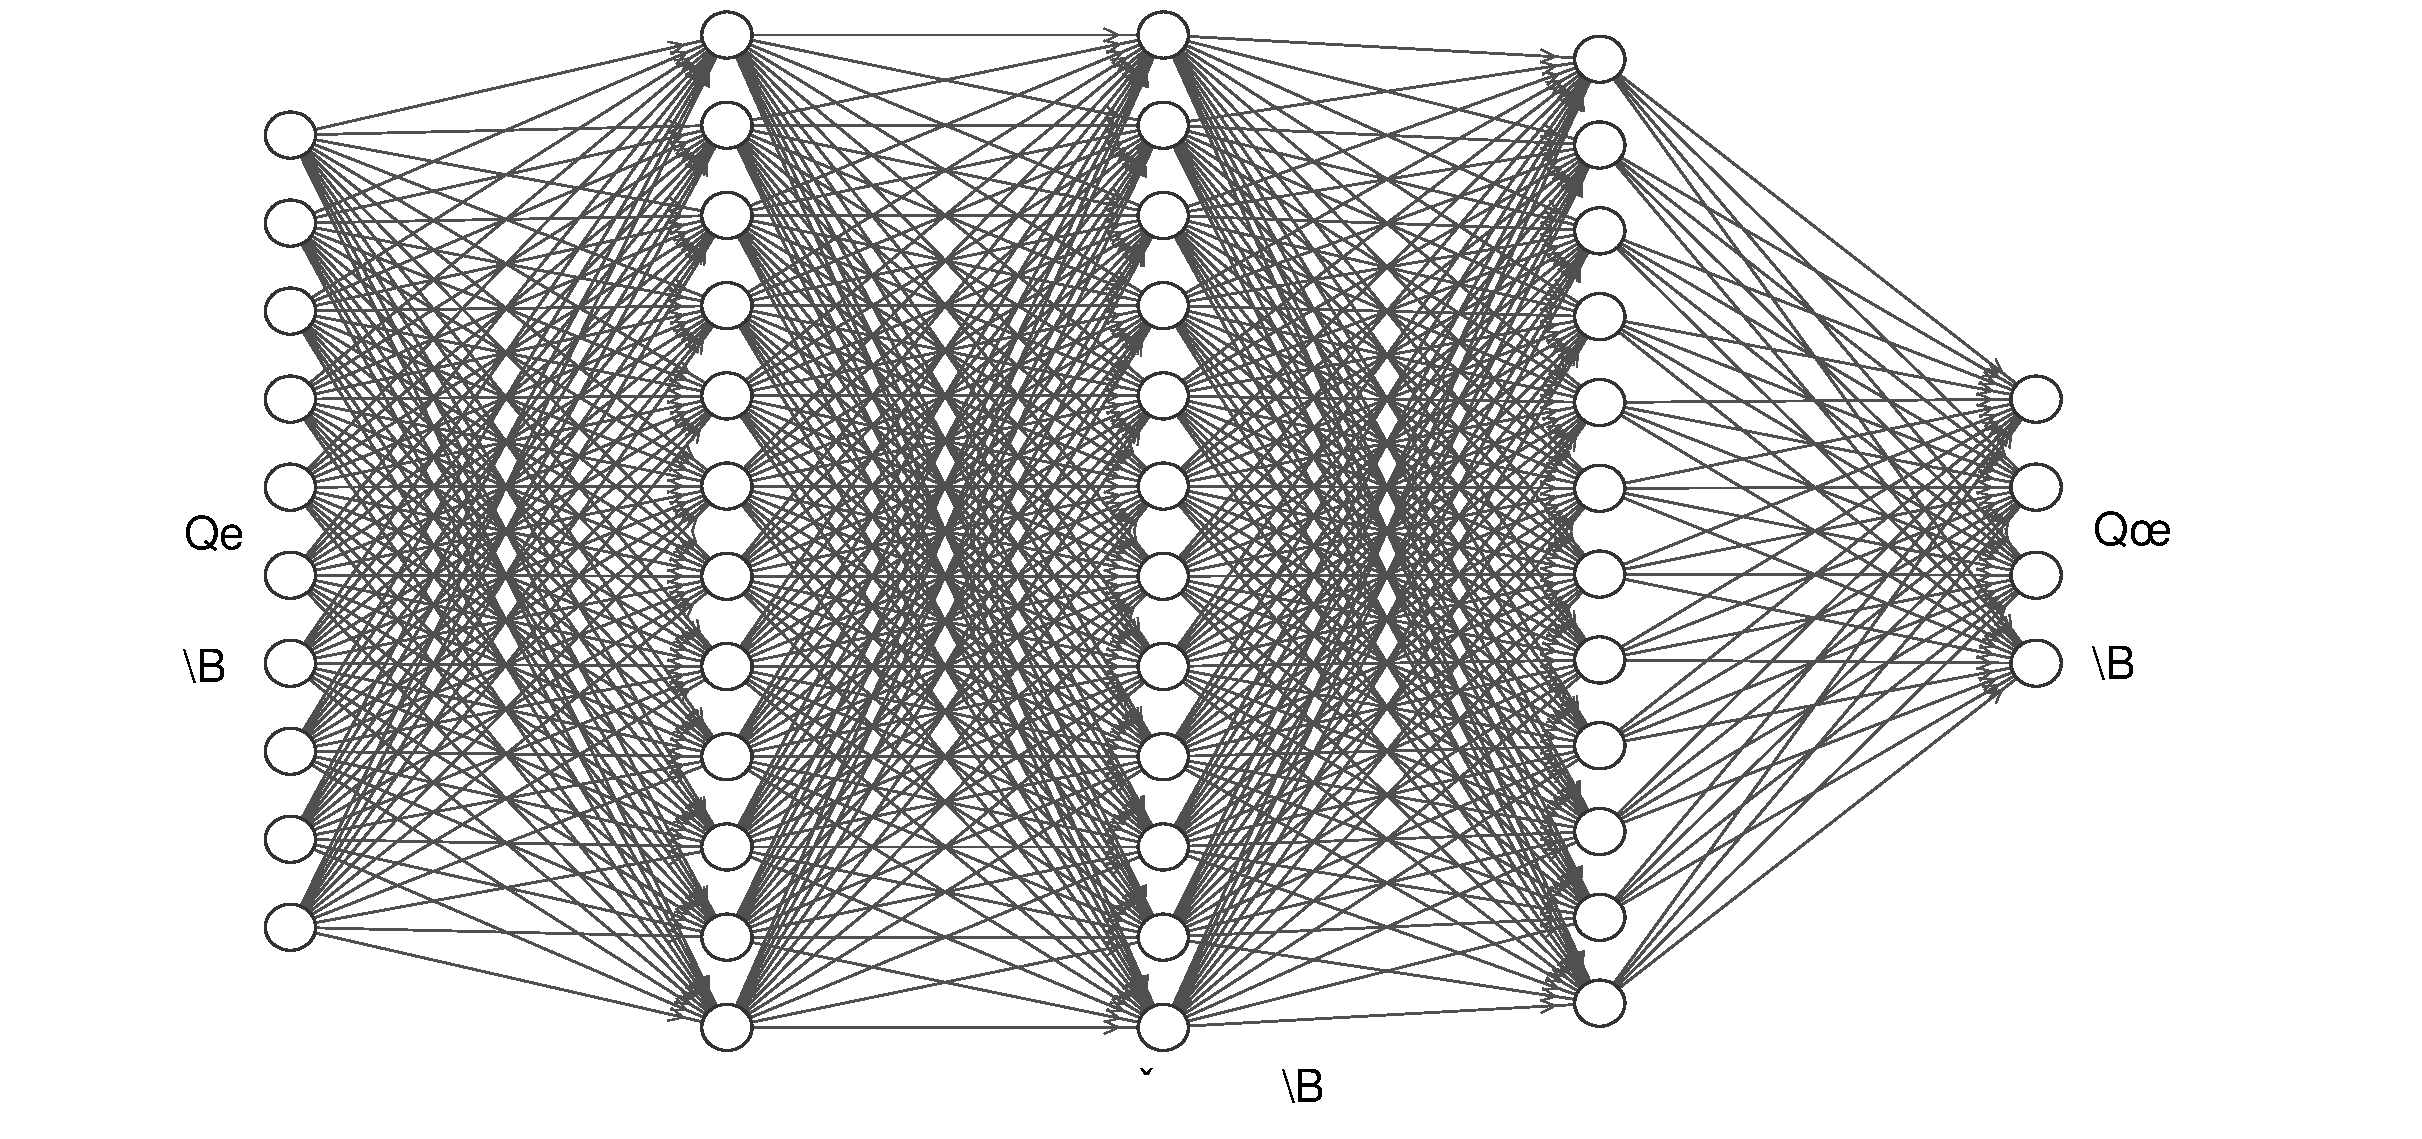
\includegraphics[width=0.9\textwidth]{nn}
    \bicaption{深度全连接网络的一般结构}{General structure of deep fully connected network}
    \label{fig:4-3}
\end{figure}

\begin{table}[!h]
    \bicaption{DNN模型结构参数表}{Structure parameter table of one-dimensional DNN model.}
    \centering
    \footnotesize
    \setlength{\tabcolsep}{15pt}
    \renewcommand{\arraystretch}{1}
\begin{tabular}{cccc}
\toprule
层数&操作&输入维度&输出维度\\
\hline
1 & input & 225 & 512 
\\ 
2 & full connect & 512 & 1024
\\ 
3 & full connect & 1024 & 1024
\\ 
4 & full connect & 1024 & 256
\\ 
5 & full connect & 256 & 128
\\ 
6 & full connect & 128 & 32
\\
7 & softmax & 32 & 5/21
\\ 
\bottomrule
\end{tabular}
\end{table}

\subsection{基于卷积神经网络的原始载荷特征挖掘模型}

%卷积神经网络是一种具有局部连接、权重共享等特性的深层前馈神经网络。卷积神经网络最早是主要用来处理图像信息。如果用全连接前馈网络来处理图像时,会存在参数太多、局部不变性特征等问题。

卷积神经网络是受生物学上感受野的机制启发而提出。感受野(Receptive Field)主要是指听觉、视觉等神经系统中一些神经元的特性,即神经元只接受其所支配的刺激区域内的信号。在视觉神经系统中,视觉皮层中的神经细胞的输出依赖于视网膜上的光感受器。视网膜上的光感受器受刺激兴奋时,将神经冲动信号传到视觉皮层,但不是所有视觉皮层中的神经元都会接受这些信号。一个神经元的感受野是指视网膜上的特定区域,只有这个区域内的刺激才能够激活该神经元。

卷积神经网络有三个结构上的特性:局部连接,权重共享以及汇聚。这些特性使得卷积神经网络具有一定程度上的平移、缩放和旋转不变性。和前馈神经网络相比,卷积神经网络的参数更少。卷积神经网络主要使用在图像和视频分析的各种任务上,比如图像分类、人脸识别、物体识别、图像分割等,其准确率一般也远远超出了其它的神经网络模型。近年来卷积神经网络也广泛地应用到自然语言处理、推荐系统等领域。

\begin{itemize}
\item 局部连接:由于图像的空间联系是局部的,每个神经元不需要对全部的图像做感受,只需要感受局部特征即可,然后在更高层将这些感受得到的不同局部神经元综合起来就可以得到全局信息,达到减少连接的数目。

\item 权重共享:不同神经元之间的参数共享可以减少模型中需要求解的参数,使用多种滤波器对数据进行卷积可以得到多种特征映射。权值共享其实是对数据用同样的卷积核进行卷积操作,使其具备平移不变性。

\end{itemize}

如图4.4所示,一般的卷积神经网络结构包括:卷积层,汇聚层和全连接层。每一层有多个特征图,每个特征图通过一种卷积滤波器提取输入特征,每个特征图有多个神经元。

\begin{figure}[!htbp]
    \centering
    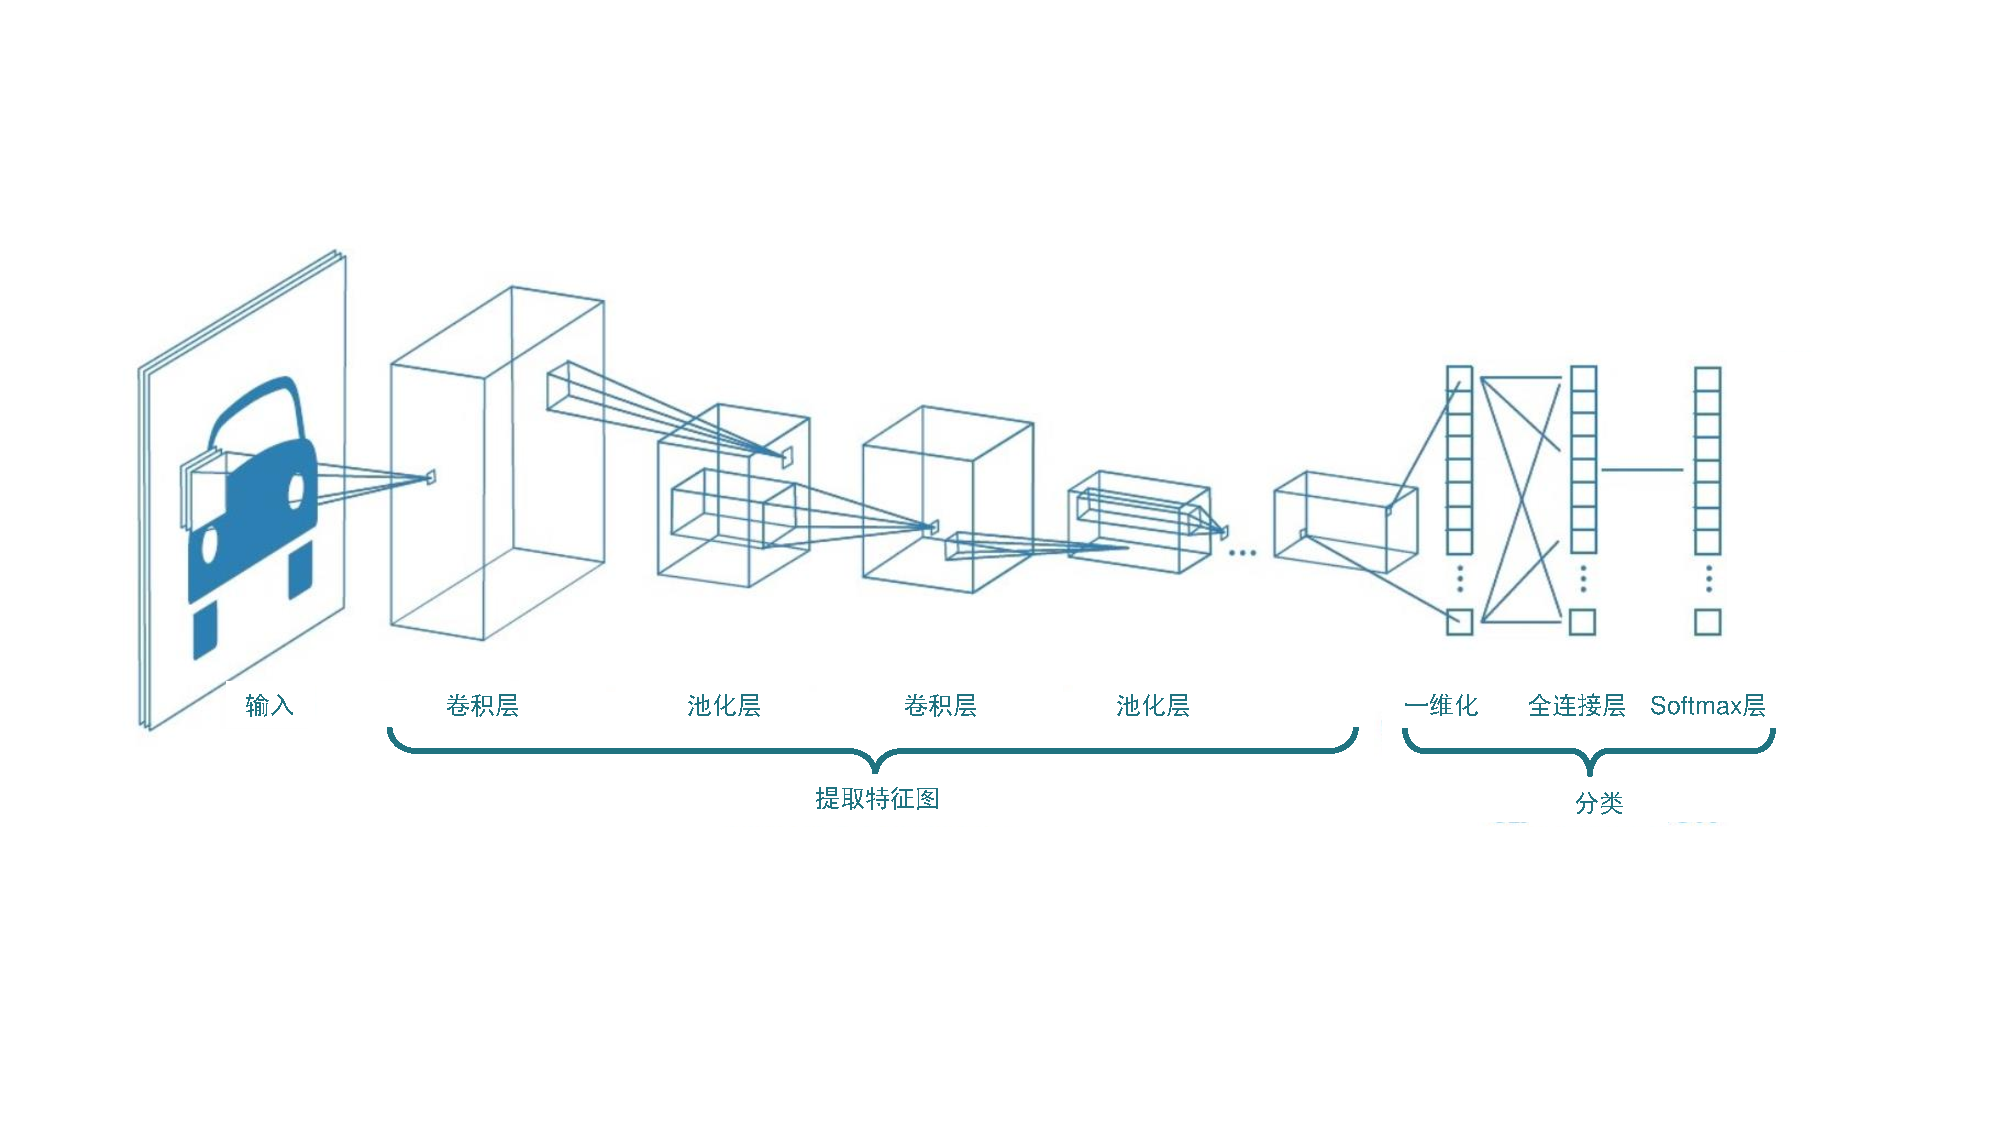
\includegraphics[width=0.8\textwidth]{4-3}
    \bicaption{卷积神经网络的一般结构}{General structure of a convolutional neural network}
    \label{fig:4-3}
\end{figure}

根据所要处理的目标不同,卷积神经网络的常见结构主要分为三种:适合处理序列数据的一维CNN,适合处理图像数据的二维CNN以及适合处理视频数据的三维CNN。在网络流量数据中,报文载荷是一种按层次结构组织的有序一维字节流,其中多个连续字节可组成有一定语义的基础字段,多个连续基础字段又可组成表示特定功能的报文片段,这种有序特性表明网络流数据属于序列数据。因此,本章选择了一维CNN模型作为进行主机属性识别效果实验,同时构建最经典的的二维CNN模型进行对比。

\begin{table}[!h]
    \bicaption{一维CNN模型结构参数表}{Structure parameter table of one-dimensional CNN model}
    \centering
    \footnotesize
    \setlength{\tabcolsep}{8pt}
    \renewcommand{\arraystretch}{1}
\begin{tabular}{ccccccc}
\toprule
层数&操作&输入维度&滤波器&步长&Pad&输出维度\\
\midrule
1 & conv+BN+ReLU & 1@1*225 & 1*3 & 1 & same & 64@1*225 
\\ 
2 & 1d max pool & 64@1*225 & 1*2 & 2 & same & 64@1*113 
\\ 
3 & conv+BN+ReLU & 64@1*113 & 1*3 & 1 & same & 128@1*113
\\ 
4 & 1d max pool &128@1*113 & 1*2 & 2 & same & 128@1*57
\\ 
5 & conv+BN+ReLU & 128@1*57 & 1*3 & 1 & same & 256@1*57
\\ 
6 & conv+BN+ReLU & 256@1*57 & 1*3 & 1 & same & 256@1*57
\\ 
7 & 1d max pool & 256@1*57 & 1*2 & 2 & same & 256@1*29
\\
8 & full connect & 256*29 & -- & -- & none & 1024
\\
9 & full connect & 1024 & -- & -- & none & 5/21
\\ 
10 & softmax & 5/21 & -- & -- & none & 5/21
\\ 
\bottomrule
\end{tabular}
\end{table}

本章构建的一维卷积神经网络模型共包含4层卷积层,3层池化层和2层全连接层,并将Softmax层作为网络的最后一层,最终得到的激活值即为模型识别出的主机属性种类。具体的参数设置如表4.2所示。其中,每层卷积层都选用ReLU函数作为激活函数,并加入了批正则处理。选择ReLU函数可以有效避免深度神经网络的梯度弥散和梯度爆炸问题,而批正则处理可以解决深度网络训练过程中难以收敛的问题,加快训练过程,并在一定程度上缓解过拟合现象。

\begin{table}[!h]
    \bicaption{二维CNN模型结构参数表}{Structure parameter table of two-dimensional CNN model}
    \centering
    \footnotesize
    \setlength{\tabcolsep}{8pt}
    \renewcommand{\arraystretch}{1}
\begin{tabular}{ccccccc}
\toprule
层数&操作&输入维度&滤波器&步长&Pad&输出维度\\
\hline
1 & conv+BN+ReLU & 1@15*15 & 2*2 & 1 & same & 64@15*15 
\\ 
2 & 2d max pool & 64@15*15 & 2*2 & 2 & same & 64@8*8 
\\ 
3 & conv+BN+ReLU & 64@8*8 & 2*2 & 1 & same & 128@8*8
\\ 
4 & conv+BN+ReLU & 128@8*8 & 2*2 & 1 & same & 256@8*8
\\ 
5 & 2d max pool & 256@8*8 & 1*2 & 2 & same & 256@4*4
\\ 
6 & full connect & 256*16 & -- & -- & none & 1024
\\ 
7 & full connect & 1024 & -- & -- & none & 5/21
\\ 
8 & softmax & 5/21 & -- & -- & none & 5/21
\\ 
\bottomrule
\end{tabular}
\end{table}

如表4.3所示,二维卷积神经网络模型主要包含3层卷积层,2层池化层和2层全连接层。同一维CNN卷积神经网络模型,每层卷积层都选用ReLU函数作为激活函数,并加入批正则处理。

\subsection{基于长短期记忆网络的原始载荷特征挖掘模型}

循环神经网络是一类具有短期记忆能力的神经网络。在循环神经网络中,神经元不但可以接受其它神经元的信息,也可以接受自身的信息,形成具有环路的网络结构。和前馈神经网络相比,循环神经网络更加符合生物神经网络的结构。循环神经网络已经被广泛应用在语音识别、语言模型以及自然语言生成等任务上。循环神经网络的参数学习可以通过随时间反向传播算法来学习。随时间反向传播算法即按照时间的逆序将错误信息一步步地往前传递。当输入序列比较长时,会存在梯度爆炸和消失问题,也称为长程依赖问题。

为了改善循环神经网络的长程依赖问题,目前最有效的改进方式就是通过引入门控机制来控制信息的累积速度,包括有选择地加入新的信息,并有选择地遗忘之前累积的信息。这一类网络可以称为基于门控的循环神经网络,最流行的代表就是长短期记忆(LSTM)网络。如图4.5所示,LSTM网络主要通过三种门实现门控机制:遗忘门、输入门和输出门。

\begin{itemize}
\item 遗忘门:控制上一个时刻的内部状态需要遗忘多少信息。
\item 输入门:控制当前时刻的输入有多少信息需要保存。
\item 输出门:控制当前时刻的内部状态有多少信息需要输出给外部状态。 
\end{itemize}

\begin{figure}[!htbp]
    \centering
    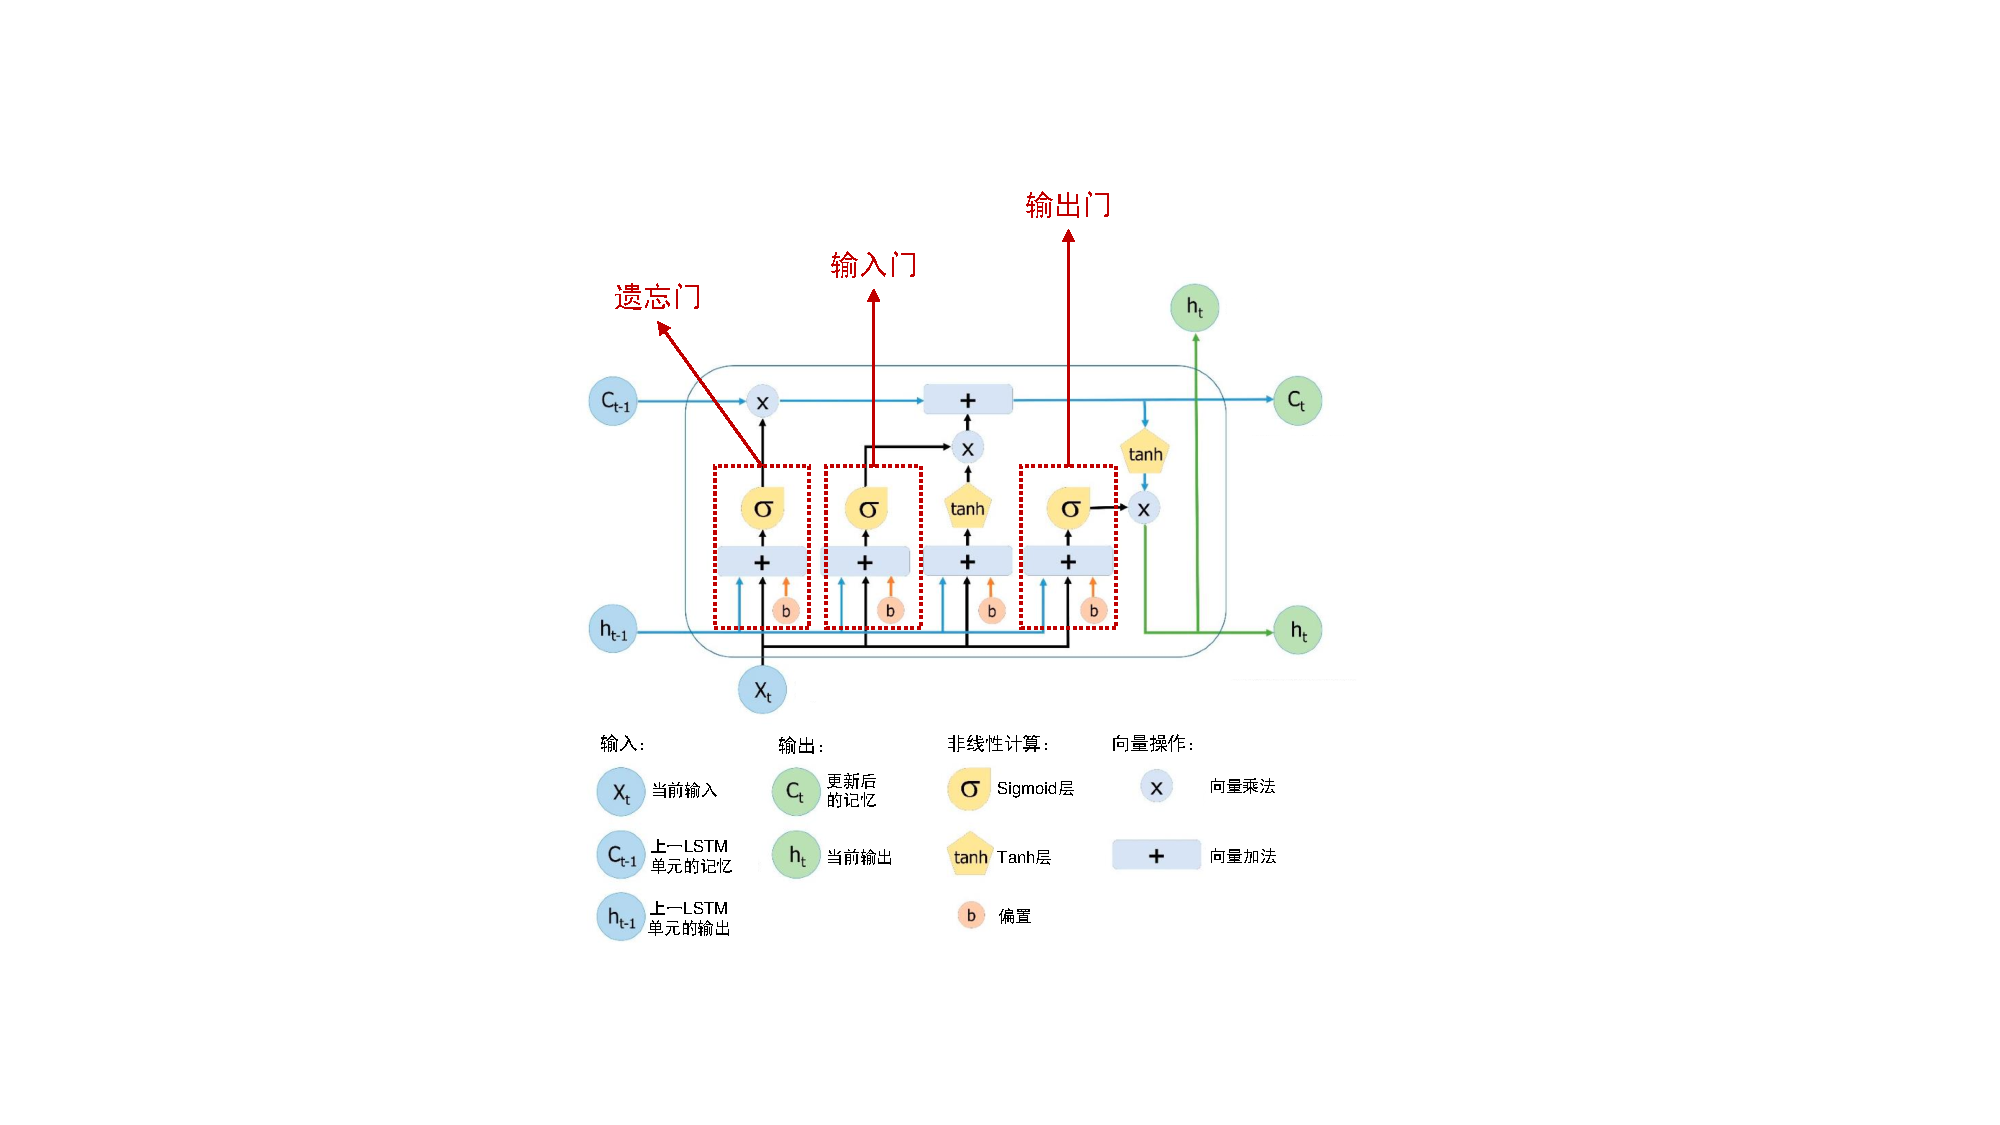
\includegraphics[width=0.7\textwidth]{4-4}
    \bicaption{LSTM网络的一般结构}{General structure of LSTM network}
    \label{fig:4-4}
\end{figure}

本章构建了一个单层LSTM网络模型,结合交叉验证法和超参数网格搜索得到的最佳模型参数如表4.4所示。其中,序列段长度为4,隐藏层节点数目为256,遗忘因子为0.1,并在输入位置添加了Dropout处理,避免过拟合问题的出现,提高模型在测试集上的性能。

\begin{table}[!htbp] 
    \bicaption{LSTM模型结构参数表}{Structure parameter table of two-dimensional LSTM model}
%    \label{tab:sample}
    \centering
    \footnotesize
    \setlength{\tabcolsep}{25pt}
    \renewcommand{\arraystretch}{1}
\begin{tabular}{lll}
\toprule
参数 & 含义 & 取值 \\ \hline
time\underline{~~}step & 序列段长度 & 4 \\ 
rnn\underline{~~}unit & 隐藏层节点数 & 256 \\ 
forget\underline{~~}bias & 遗忘因子 & 0.1 \\ 
\bottomrule
\end{tabular}
\end{table}

\subsection{模型效果对比}

为了选择适合主机属性发现任务的最佳深度学习模型,本节从分类准确率、精度、召回率以及PR曲线等角度对深度全连接网络、一维卷积神经网络、二维卷积神经网络以及长短期记忆网络等模型进行效果对比实验。同时,为了展示基于加密流原始载荷的主机属性方法的优越性,引入第三章中基于人工特征的最优模型即LightGBM模型共同进行对比实验。本节实验均采用Tensorflow框架来实现各种深度学习模型,其他实验环境参数详情以及数据集详情参照3.4节和3.5节。

\begin{figure}[!h]
    \centering
    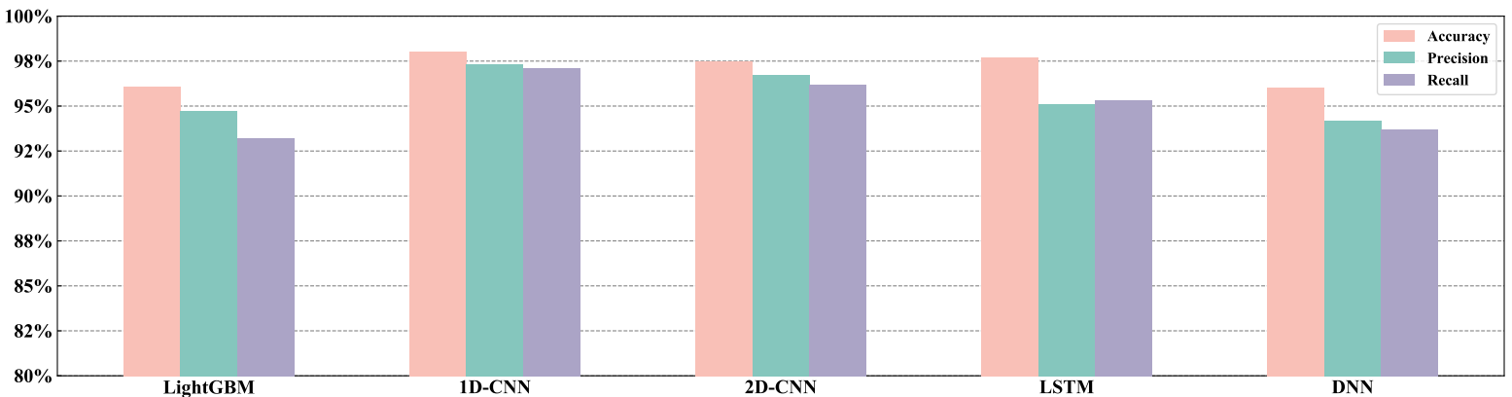
\includegraphics[width=0.9\textwidth]{4-5}
    \bicaption{模型准确率、精度和召回率对比}{Comparison of model accuracy, precision and recall}
    \label{fig:4-4}
\end{figure}

\begin{figure}[!h]
    \centering
    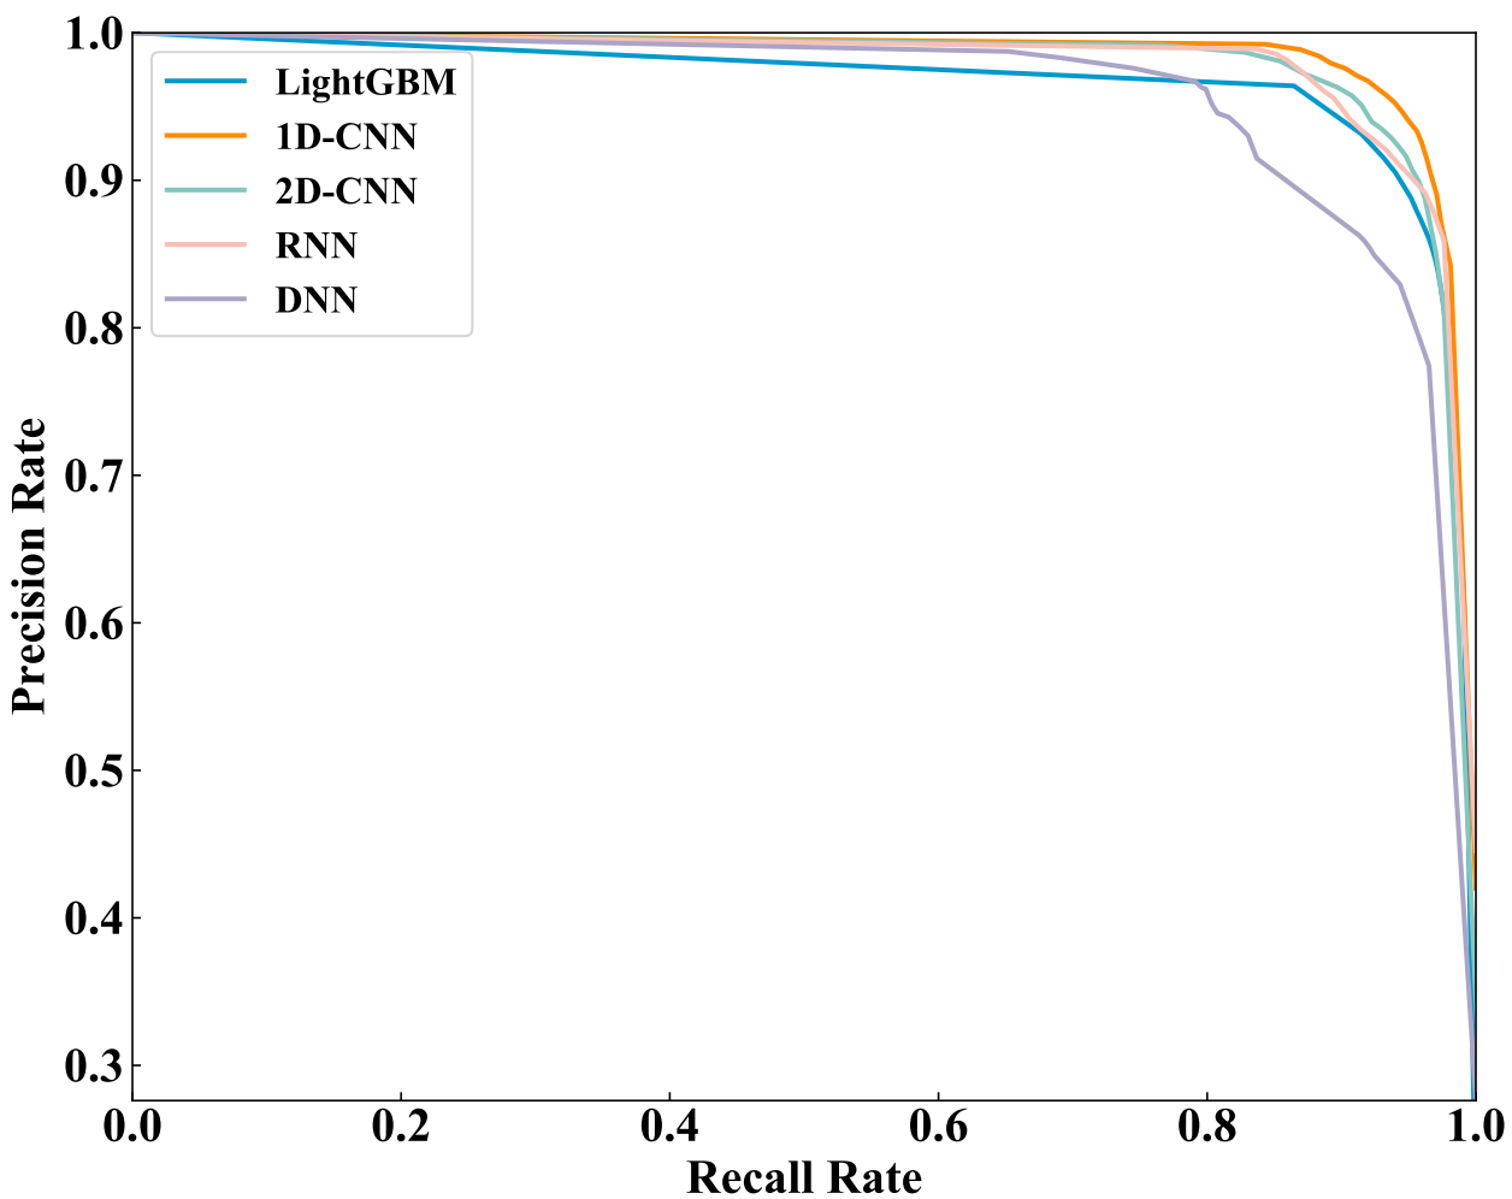
\includegraphics[width=0.6\textwidth]{4-6}
    \bicaption{模型PR曲线对比}{Model PR curve comparison}
    \label{fig:4-4}
\end{figure}

如图4.6和4.7所示,从准确率、精度、召回率和PR曲线等评估指标来看,一维CNN模型在众多神经网络模型中有着最佳表现。而且和从人工特征数据集中训练出的LightGBM模型相比,一维CNN模型的准确率、精度和召回率都提高了近3\%,PR曲线也完全包住了LightGBM模型的PR曲线。以上实验结果都证明一维CNN模型是最适合主机属性发现任务的神经网络模型。



\section{基于加密流原始载荷的主机属性发现结果}

基于加密流原始载荷的主机属性发现技术以一维卷积神经网络作为分类器,将TCP SYN包和TLS Clinet Hello包的原始流信息经过数据归一化处理后作为输入,便可识别目标主机的各种属性。

将数据集按照日期进行切分,以前四天的数据作为训练集,以最后一天的数据作为测试集,可得到如表4.5-4.7的识别结果。

\begin{table}[!h]
    \bicaption{操作系统类型识别结果}{Operating system type identification results}
    \centering
    \footnotesize
    \setlength{\tabcolsep}{8pt}
    \renewcommand{\arraystretch}{1}
\begin{tabular}{|c|c|c|c|c|c|c|c|}
\hline
\multirow{2}{*}{ \textbf{ID}} & \multirow{2}{*}{ \textbf{操作系统类型}} & \multicolumn{3}{c|}{ \textbf{训练集}} & \multicolumn{3}{c|}{ \textbf{测试集}} \\ \cline{3-8} 
 &  &  \textbf{Precision} &  \textbf{Recall} &  \textbf{F1} & \textbf{Precision} &  \textbf{Recall} &  \textbf{F1} \\ \hline
1 & Android & 98.10\% & 98.07\% & 98.08\% & 97.86\% & 97.85\% & 97.86\% \\ \hline
2 & iOS & 77.29\% & 75.88\% & 76.58\% & 74.15\% & 70.82\% & 72.45\% \\ \hline
3 & Windows & 97.87\% & 98.23\% & 98.05\% & 97.54\% & 97.95\% & 97.74\% \\ \hline
4 & MacOS & 99.21\% & 97.61\% & 98.40\% & 99.03\% & 97.79\% & 98.40\% \\ \hline
5 & Linux & 99.64\% & 99.25\% & 99.44\% & 99.37\% & 98.84\% & 99.10\% \\ \hline
\multicolumn{2}{|c|}{\textbf{AVE}} & 94.42\% & 93.81\% & 94.11\% & 93.59\% & 92.65\% & 93.11\%\\ \hline
\multicolumn{2}{|c|}{\textbf{Accuracy}} & \multicolumn{3}{c|}{98.79\%} & \multicolumn{3}{c|}{98.17\%} \\ \hline
\end{tabular}
\end{table}

在操作系统类型识别任务中,Linux系统的识别效果最好,精度为99.37\%,召回率为98.84\%,F1分数为99.10\%,远高于平均值。由在4.2节中分析的Linux系统原始流量灰度图可知,其TLS协议中存在一个区分度非常高的重协商信息扩展,使得Linux系统的样本容易被分类器识别。iOS系统的识别效果最差,F1分数仅有72.45\%,可能是因为iOS系统原始流量的局部特征不够明显导致。

\begin{table}[!h]
    \bicaption{操作系统版本识别结果}{Operating system version identification results}
    \centering
    \footnotesize
    \setlength{\tabcolsep}{8pt}
    \renewcommand{\arraystretch}{1}
\begin{tabular}{|c|c|c|c|c|c|c|c|}
\hline
\multirow{2}{*}{\textbf{ID}} & \multirow{2}{*}{\textbf{操作系统版本}}  & \multicolumn{2}{c|}{\textbf{测试集}} & \multirow{2}{*}{\textbf{ID}} & \multirow{2}{*}{\textbf{操作系统版本}}  & \multicolumn{2}{c|}{\textbf{测试集}} \\ \cline{3-4} \cline{7-8}
 &  & \textbf{Precision} & \textbf{Recall}  & & & \textbf{Precision} & \textbf{Recall} \\ \hline
1 & Android 4 & 78.99\% & 61.58\% &12 & iOS 7 & 98.86\% & 98.86\% \\ \hline
2 & Android 5 & 83.90\% & 74.63\% &13 & iOS 8 & 36.36\% & 30.77\% \\ \hline
3 & Android 6 & 88.21\% & 77.85\% &14 & iOS 9 & 80.30\% & 77.94\% \\ \hline
4 & Android 7 & 92.18\% & 62.48\% &15 & iOS 10 & 61.54\% & 53.33\% \\ \hline
5 & Android 8 & 63.68\% & 78.11\% &16 & iOS 11 & 77.01\% & 80.72\% \\ \hline
6 & Android 9 & 66.73\% & 72.05\% &17 & iOS 12 & 40.06\% & 66.83\% \\ \hline
7 & Windows XP & 85.40\% & 76.35\% &18 & MacOS 10 & 98.87\% & 99.15\% \\ \hline
8 & Windows 7 & 92.41\% & 92.96\% &19 & MacOS 11 & 99.63\% & 99.57\% \\ \hline
9 & Windows 8 & 100.00\% & 36.59\% &20 & MacOS 12 & 98.61\% & 91.03\% \\ \hline
10 & Windows 8.1 & 97.30\% & 80.45\% &21 & Ubuntu & 99.51\% & 99.12\% \\ \hline
11 & Windows 10 & 95.94\% & 97.66\% & \multicolumn{2}{c|}{\textbf{AVE}}& 78.78\% & 73.04\% \\ \hline
\end{tabular}
\end{table}

在操作系统版本识别任务中,总体识别效果要明显差于操作系统类型识别任务结果,这是因为操作系统版本识别任务是一个细粒度主机属性识别任务,本质上是一个21类分类任务,而操作系统类型识别任务是一个5类分类任务。一般而言,对于同等规模的训练数据集,深度学习模型的预测能力与预测类别数目成反比。在具体识别结果中,Windows8系统的识别精度为100\%,召回率却只有36.59\%,精度和召回率相差十分明显的原因主要有两个,一个是Windows 8的样本量在数据集中的比例较小,第二个原因是Windows 8和Windows 8.1的网络协议栈实现差异性较小,在协议指纹上的区分度不明显,导致了其识别召回率非常差。同样的问题也存在于部分iOS系统的版本识别结果中。

\begin{table}[!h]
    \bicaption{浏览器类型识别结果}{Browser type identification results}
    \centering
    \footnotesize
    \setlength{\tabcolsep}{8pt}
    \renewcommand{\arraystretch}{1}
\begin{tabular}{|c|c|c|c|c|c|c|c|}
\hline
\multirow{2}{*}{ \textbf{ID}} & \multirow{2}{*}{ \textbf{浏览器类型}} & \multicolumn{3}{c|}{ \textbf{训练集}} & \multicolumn{3}{c|}{ \textbf{测试集}} \\ \cline{3-8} 
 &  &  \textbf{Precision} &  \textbf{Recall} &  \textbf{F1} & \textbf{Precision} &  \textbf{Recall} &  \textbf{F1} \\ \hline
1 & Firefox & 97.90\% & 88.50\% & 92.96\% & 97.12\% & 86.33\% & 91.41\% \\ \hline
2 & Safari & 94.72\% & 88.76\% & 91.64\% & 94.32\% & 85.79\% & 89.85\% \\ \hline
3 & Chrome & 97.68\% & 99.52\% & 98.59\% & 97.42\% & 99.43\% & 98.41\% \\ \hline
4 & IE & 94.66\% & 77.24\% & 85.07\% & 92.91\% & 75.78\% & 83.48\% \\ \hline
5 & Opera & 91.37\% & 89.70\% & 90.13\% & 95.81\% & 87.47\% & 90.66\% \\ \hline
\multicolumn{2}{|c|}{\textbf{AVE}} & 95.27\% & 88.74\% & 91.68\% & 95.52\% & 86.96\% & 90.76\%\\ \hline
\multicolumn{2}{|c|}{\textbf{Accuracy}} & \multicolumn{3}{c|}{97.43\%} & \multicolumn{3}{c|}{97.10\%} \\ \hline
\end{tabular}
\end{table}

在浏览器类型识别任务中,Chrome浏览器的识别效果最佳,精度为97.42\%,召回率为99.43\%,F1分数为98.41\%。相对于利用人工提取特征的机器学习模型,神经网络模型对于Chrome浏览器的识别精度明显提升,充分体现了表示学习的优越性。IE浏览器的识别效果相对较差,F1分数为83.48\%,可能是由于其原始字节序列中的局部特征较少。

\section{本章小结}

本章介绍了基于加密流原始载荷的主机属性发现技术,利用表示学习的思想,不需要任何专家知识,只需将网络流的原始流数据作为分类器输入,便可完成细粒度的主机属性发现,并拥有相对于传统方法更佳的识别效果。对于各种流行的深度学习模型,通过分组实验对比在主机属性识别任务中的各类评估指标,发现一维卷积神经网络的适应性最佳。在识别任务的实验结果中,该技术在准确率、精度、召回率以及F1值等方面,效果均优于基于TCP/IP协议栈指纹的LightGBM模型。



\chapter{主机属性识别系统的设计与实现}

为了可以从实时网络中进行大规模的细粒度主机属性识别,本章基于前文的研究成果,设计并实现了一套原型系统,可在真实网络中较为准确地识别客户端主机的操作系统种类、版本以及浏览器种类等属性,并具备网络协议识别与解析、TLS流数据属性标注、日志信息存储与查询、主机属性发现实时可视化等功能。本章首先介绍系统的设计原则与目标,展示主机属性识别系统的组织架构、主要模块与功能。然后详细介绍各个模块的具体实现和关键算法。最终在开放网络中部署完整的原型系统,并从多个角度测试系统效果与性能。

\section{设计原则与目标}

在原型系统设计之前,为了更高效率的开发,本章提出了五项设计原则作为指导,分别是准确率高,隐蔽性强,识别范围广,处理速度快,结果可存储、查询和分析等。
\begin{itemize}

\item
准确率高。主机属性识别作为网络攻防的首要任务,识别的准确率、精度和召回率等指标关系着后续步骤的实施效果,决定了整个攻防任务的成败,是设计目标中的重中之重。
\item
隐蔽性强。在识别过程中应避免引起检测对象的察觉,由于本文采用被动识别方法,只需利用网络嗅探技术从网络节点中捕获流量,本身的隐蔽性能已经满足需求。
\item
识别范围广。传统主机属性识别方法多依赖于指纹库匹配,对于匹配失败的未知指纹无法进行有效识别。原型系统应摒弃指纹库的搭建,利用机器学习模型学习主机指纹的样本空间,具备较强的灵活性。
\item
处理速度快。原型系统将部署在大规模的网络中,必须具备适应高速流量的吞吐量。
\item
结果可存储、查询和分析。在对大规模网络中的主机属性进行识别后,预测结果可以保存在数据库中,并且利用可视化技术向用户提供图形界面,完成识别结果的简单分析。
\end{itemize}

\section{原型系统的组织架构}

本原型系统由五部分模块组成,包括流量采集模块、特征提取模块、属性识别模块、分类器更新模块以及数据存储与可视化模块。系统的组织结构如图5.1所示。

\begin{figure}[!h]
    \centering
    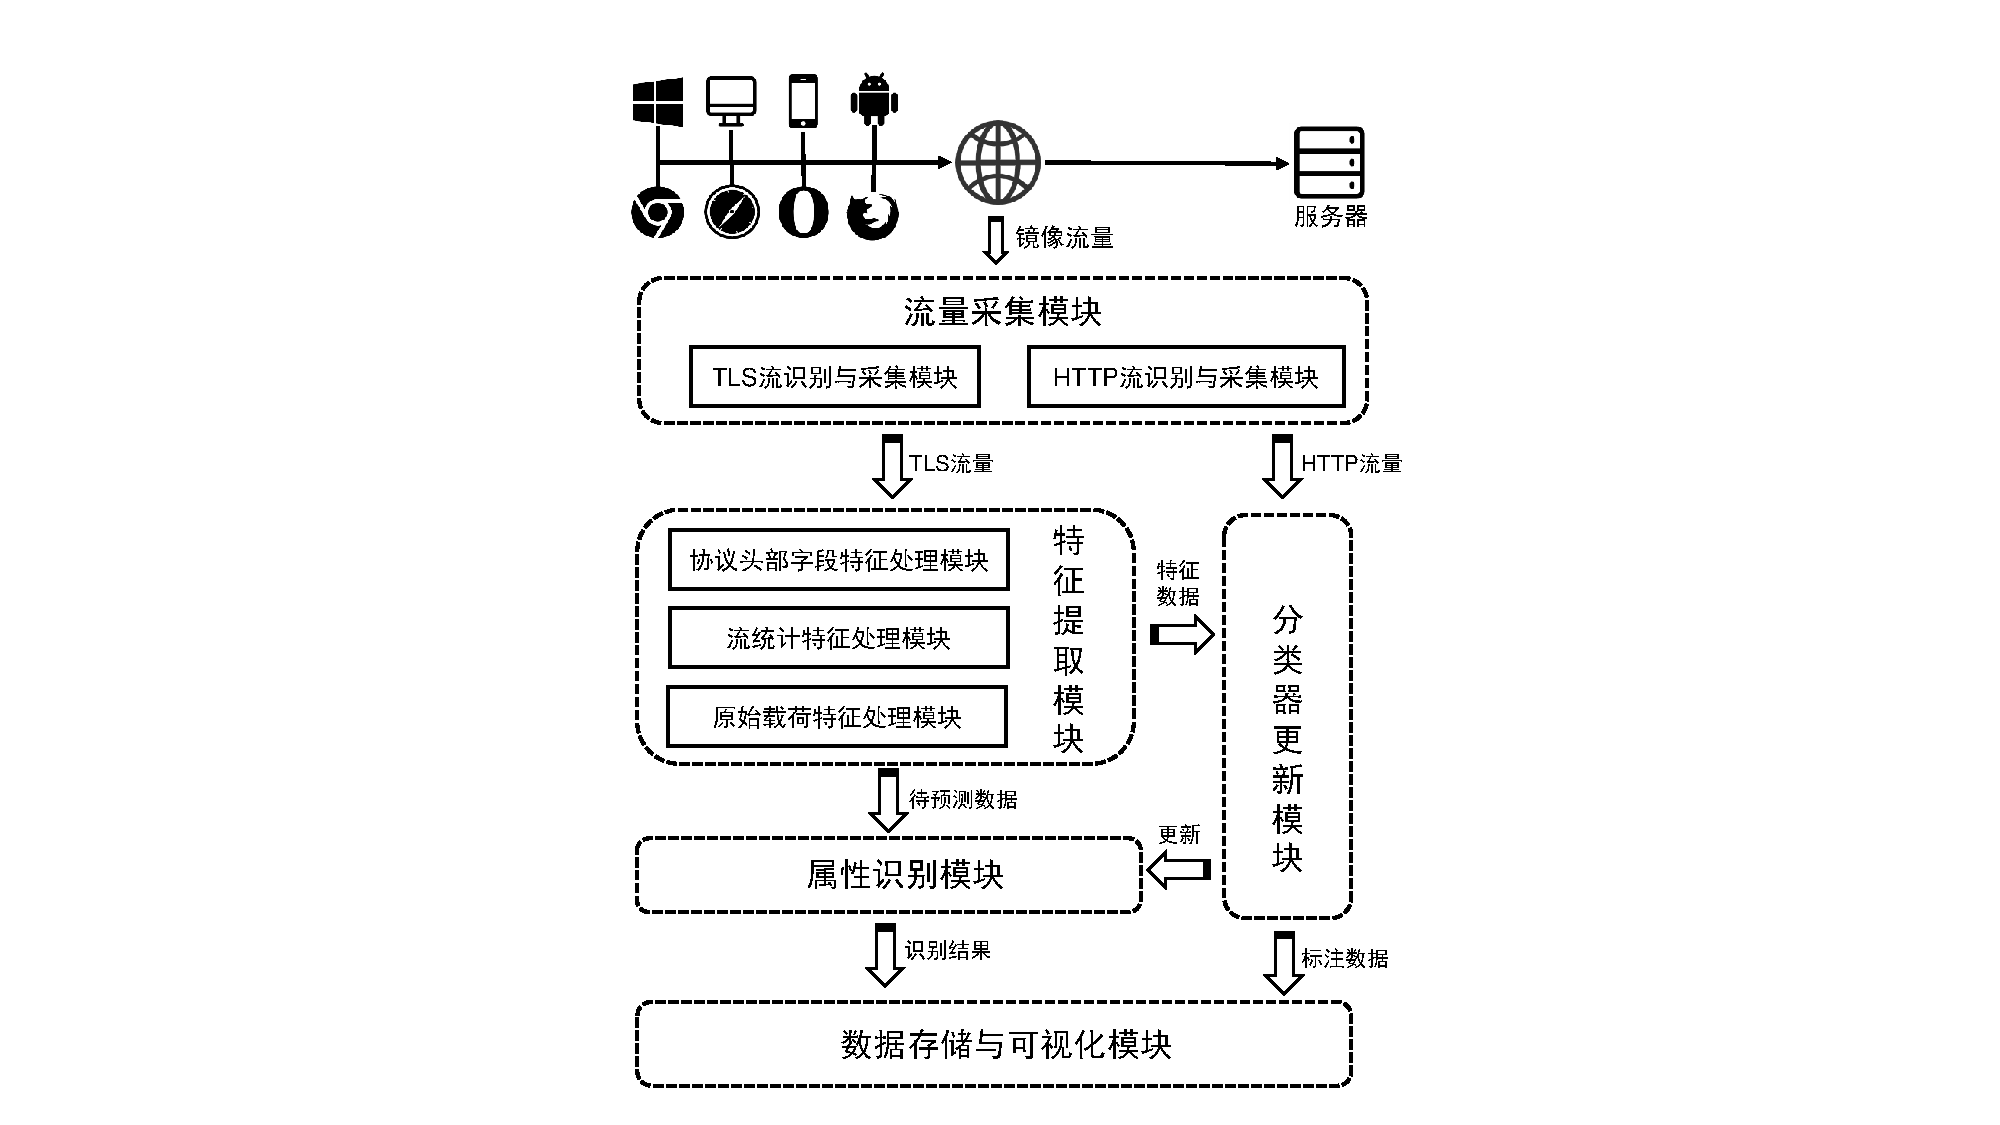
\includegraphics[width=0.7\textwidth]{原型系统架构}
    \bicaption{系统的组织架构}{Organizational structure of the system}
    \label{fig:5-1}
\end{figure}

流量采集模块:从实时网络中识别目标协议网络会话,并将同一会话的所有报文按序汇聚为双向流。

特征提取模块:对网络流数据进行格式解析,提取所需协议首部字段特征,统计网络流前50个数据包的长度序列特征和时间序列特征,对此类人工特征进行数据预处理后传递给属性识别模块中的集成树模型。此外,拼接TCP SYN包和TLS Client Hello包的原始字节数据并进行归一化处理,然后传递给属性识别模块中的神经网络模型进行属性预测。

属性识别模块:为了综合统计机器学习模型和深度学习模型的优点,利用Stacking技术将多个集成树模型和神经网络模型进行融合,进一步提升识别效果。

分类器更新模块:由于训练后的分类器只能识别已知的主机属性类型,为了增强系统的可扩展性,分类器更新模块可以从客户端的HTTP请求中解析出客户端主机信息,并将之与同一客户端的TLS流进行关联,构造有标签的训练数据集。并结合已有的数据集,对属性识别模块中的第一层模型进行离线训练,使得更新后的模型可识别更多的主机属性类别。

数据存储与可视化模块:首先利用Logstash数据采集引擎收集属性识别模块产生的结果日志,然后将Elasticsearch作为数据库和检索工具,最后使用Kibana工具从结果数据中生成Web界面,完成可视化功能。

本系统的工作流程是先由流量采集模块从目标网络中被动收集镜像流量,以双向流为单位给其他模块提供原始数据来源。特征提取模块通过解析获取的TLS流数据,得到协议字段特征、流统计特征以及原始字节数据,在经过数据预处理和特征转换后,为其他模块提供特征数据来源。属性识别模块和分类器更新模块分别基于特征数据进行预测和训练,同时离线训练模块中的模型可以根据需要为属性识别模块中的模型提供更新。最终,属性识别模块的预测结果由数据存储与可视化模块进行存储、查询与可视化。

\section{流量采集模块}

流量采集模块主要负责从网络中识别和采集HTTP流量和TLS流量,模块内结构如图5.2所示。按照RFC文档规定,HTTP协议的服务端口一般为80端口,TLS协议的服务端口一般为443端口。因此,本模块首先基于端口识别目标流量,然后以五元组<客户端IP, 服务端IP, 客户端端口, 服务端端口,传输层协议类型>为单位将每个网络会话的数据包汇聚为双向流,同时记录每个数据包的捕获时间以形成包到达时间序列,再根据RFC文档中协议格式的定义对数据包进行解析,丢弃协议格式异常的网络流。最终,将过滤后的目标流量及其包到达时间序列传输到特征提取模块和分类器更新模块。

\begin{figure}[!h]
    \centering
    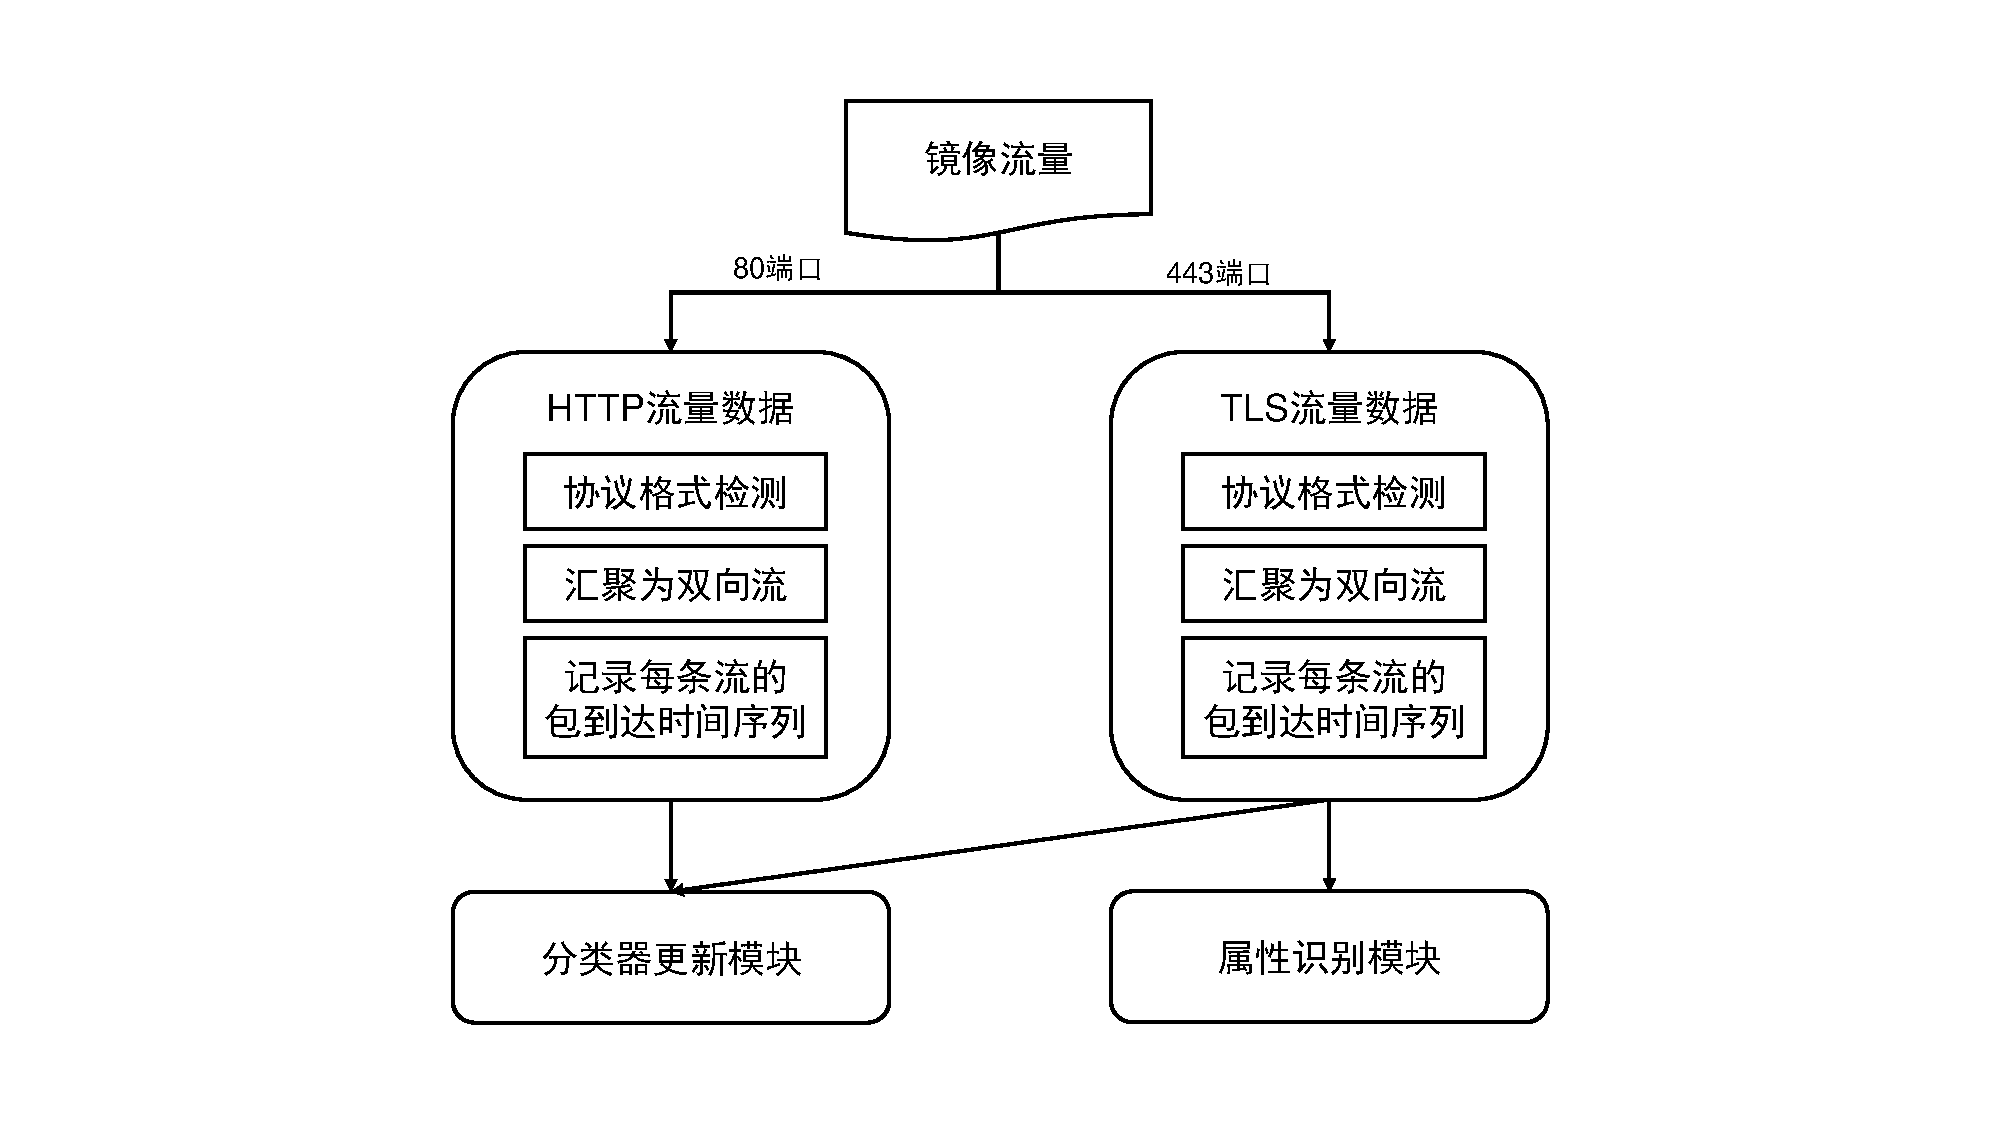
\includegraphics[width=0.6\textwidth]{流量采集模块}
    \bicaption{流量采集模块}{Traffic collection module}
    \label{fig:5-2}
\end{figure}

\section{特征提取模块}

在获取TLS流量后,特征提取模块根据协议格式标准对每条双向流的所有报文进行格式解析。当判定目标流量没有异常后,筛选出每条双向流地TCP SYN包和TLS Client Hello包以供接下来的各特征提取模块使用,其工作流程如图5.3所示。

\begin{figure}[!htbp]
    \centering
    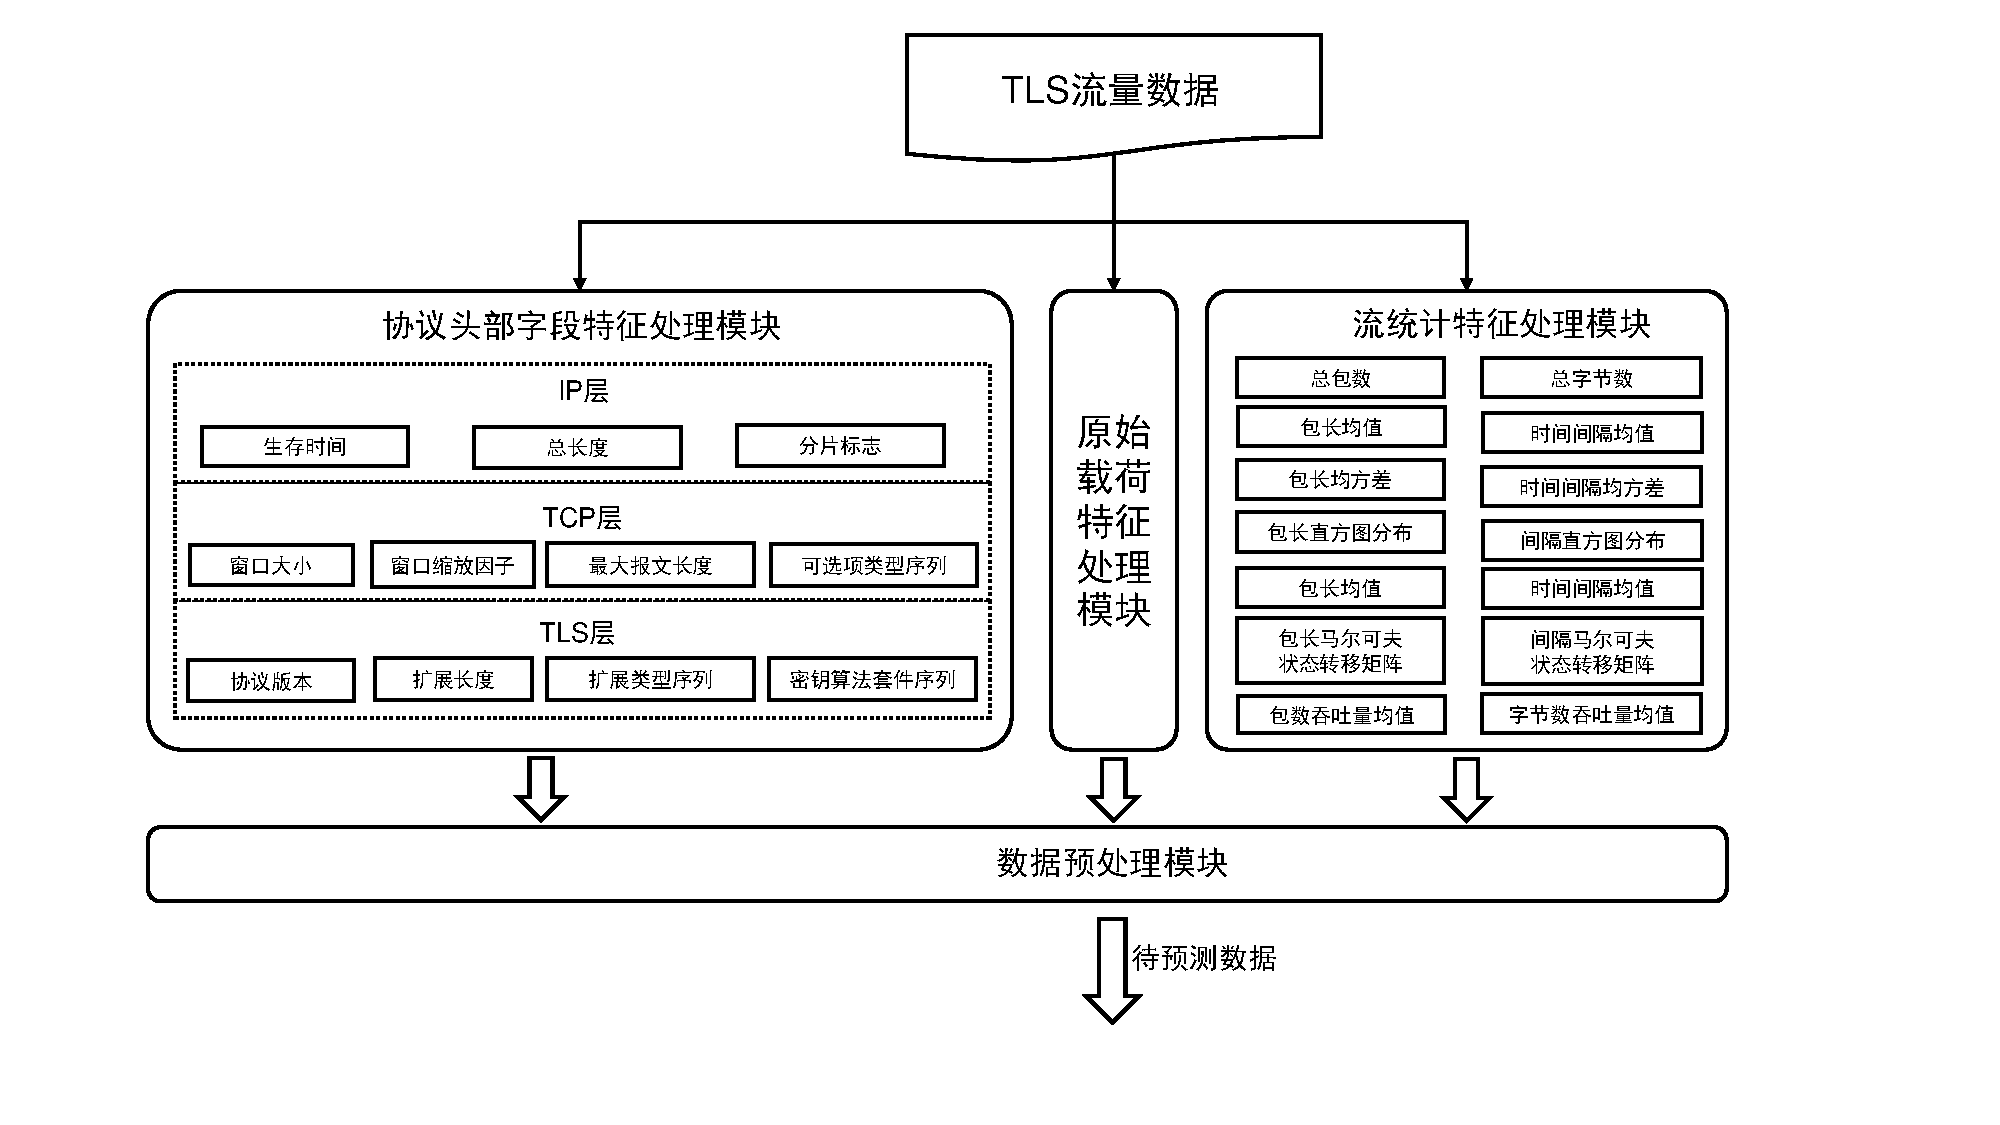
\includegraphics[width=0.9\textwidth]{特征提取模块}
    \bicaption{特征提取模块}{Feature extraction module}
    \label{fig:5-2}
\end{figure}

协议头部字段特征处理模块主要从TCP SYN包中提取IP协议首部的生存时间、总长度、分片标志等字段信息和TCP协议首部的窗口大小、窗口缩放因子、最大报文长度、可选项类型序列等字段信息,从TLS Client Hello包中提取协议版本、密钥算法套件序列、扩展长度、扩展类型序列、支持加密组件序列以及应用层协议协商状态码序列等字段信息。接着对于以上十三维特征进行各种数据预处理操作,包括缺失值填充,异常值处理,字符串特征编码等,得到可直接作为机器学习模型输入的十三维离散特征。

流统计特征处理模块的功能是提取和处理TLS流前50个包的包长序列特征和包到达时间序列特征。包长序列可由50个包的每包长度直接获取,通过计算便可得到包长均值、均方差、直方图分布和马尔可夫状态转移矩阵等统计特征。包到达时间序列由流量采集模块记录并提供,根据包到达时间序列可以计算得到包到达时间间隔均值、均方差、直方图分布和间隔马尔可夫状态转移矩阵等统计特征。最后通过统计完整流的所有报文信息,可得到总包数、总字节数、包数吞吐量均值、字节数吞吐量均值以及传输峰值分布等特征。对于以上连续特征进行数据归一化处理后,得到可作为机器学习模型输入的420维特征。

原始载荷特征处理模块的功能较为简单,主要从TCP SYN包中提取出IP层和TCP层的首部原始字节,从TLS Client Hello包中提取出TLS层的首部原始字节,对以上字节按序拼接在一起,并设置长度阈值为500字节,对长度大于500的原始字节序进行截断处理,对长度小于500的原始字节序进行填零补充。最终将长度为500的原始字节序进行归一化处理后,便可得到作为深度学习模型输入的500维特征。

\section{属性识别模块}

由于在实际的学习任务中,很难找到一个稳定性和预测性能都令人满意的模型,因此本系统的属性识别模块采用了双层结构的集成机器学习分类器。集成学习通过融合多个基模型,可以得到一个泛化性能更好的集成模型。在本模块中,第一层模型分别是以协议首部字段特征、流统计特征为输入的集成树模型和以原始字节序为输入的神经网络模型,第二层模型是以第一层模型预测结果为输入的逻辑回归模型。集成树模型包括3.3节中介绍的RF模型和LightGBM模型,神经网络模型包括4.2节中介绍的一维CNN模型和LSTM模型。

\begin{figure}[!h]
    \centering
    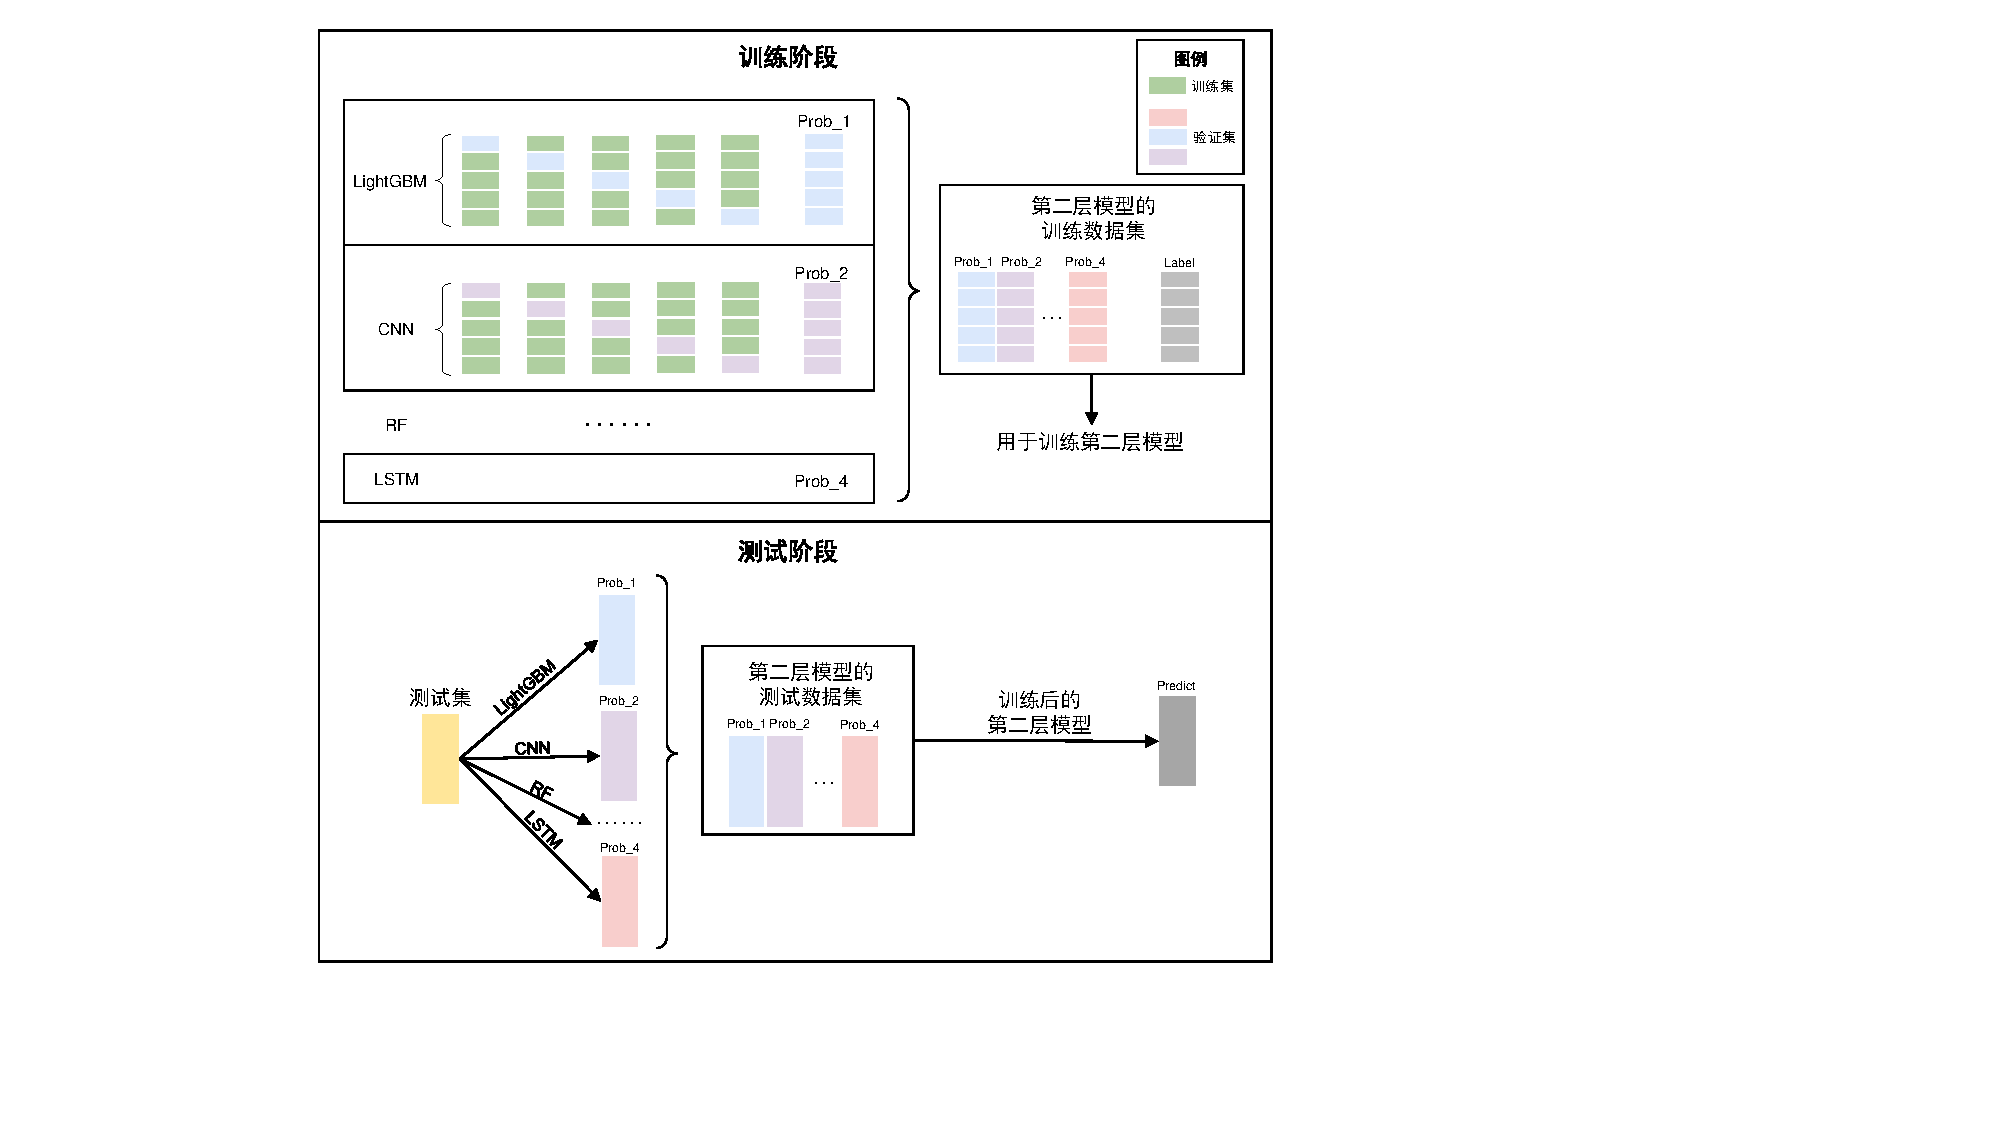
\includegraphics[width=0.9\textwidth]{stacking2}
    \bicaption{Stacking算法原理}{Stacking algorithm principle}
    \label{fig:5-3}
\end{figure}

本模块集成方法利用的主要思想是Stacking算法,和深度学习算法类似,Stacking算法也是一种表示学习算法,通过训练高层模型学习使用基模型的预测数据,可以实现对基模型的选择性表达,是目前提升机器学习效果最好的算法之一。Stacking算法原理如图5.4所示,在训练阶段中,首先利用K折交叉验证将原始训练集切分为K个子集,图中K值为5,然后将每个基模型训练并预测K次,每次训练循环以1个子集为验证集,以其余子集为训练集,最终得到四个模型在训练集上的类别预测概率数据,即为高层模型的训练特征数据。结合原始训练集中的标签数据,便可完成对高层模型的训练。

在测试阶段中,对于单个模型,利用其在K折交叉验证中的K次训练,可以对测试集数据进行预测K次,然后取这K次预测概率结果的均值,得到单个模型对测试集的类别预测概率数据。然后拼接所有基模型的预测概率数据,作为高层模型的预测特征数据。最后利用训练后的高层模型对特征数据进行预测,即可得到集成模型对测试集中所有样本的分类结果。
%将每个模型的预测结果拼接后得到Stacking训练集。同理,将K折交叉验证过程中每次训练后的基模型对原始测试集进行预测,最后取均值后得到Stacking测试集。在第二层模型中,通常选用原理和结构简单的机器学习模型从第一层的模型输出中学习有效特征,类似于投票器,本质是对第一层模型预测结果的权重学习。

%同其他集成学习方法一样,为了得到更强的泛化性能,进行Stacking集成时要求基学习器尽量保持独立,且效果相近。在3.4节的对比实验中可以看到,RF模型、XGBoost模型和LightGBM模型性能都比较优秀,但RF模型是基于Bagging算法,XGBoost模型和LightGBM模型都是基于Boosting算法,原理近似,因此本模块选择RF模型、LightGBM模型、一维卷积神经网络模型和长短期记忆网络模型等四种原理不同、性能优秀的模型作为基学习器。

属性识别模块利用以上介绍的集成分类器,可高效、精准地从样本数据中识别出每条加密流的客户端主机属性,目前主机属性包括操作系统种类、版本以及浏览器种类。未来可根据需求,结合分类器更新模块,扩展识别种类更多、粒度更细的主机属性。

\section{分类器更新模块}

分类器更新模块的功能是为属性识别模块中的分类器提供模型更新和优化服务,本质是对集成分类器的再训练过程,工作流程如图5.5所示。

\begin{figure}[!htbp]
    \centering
    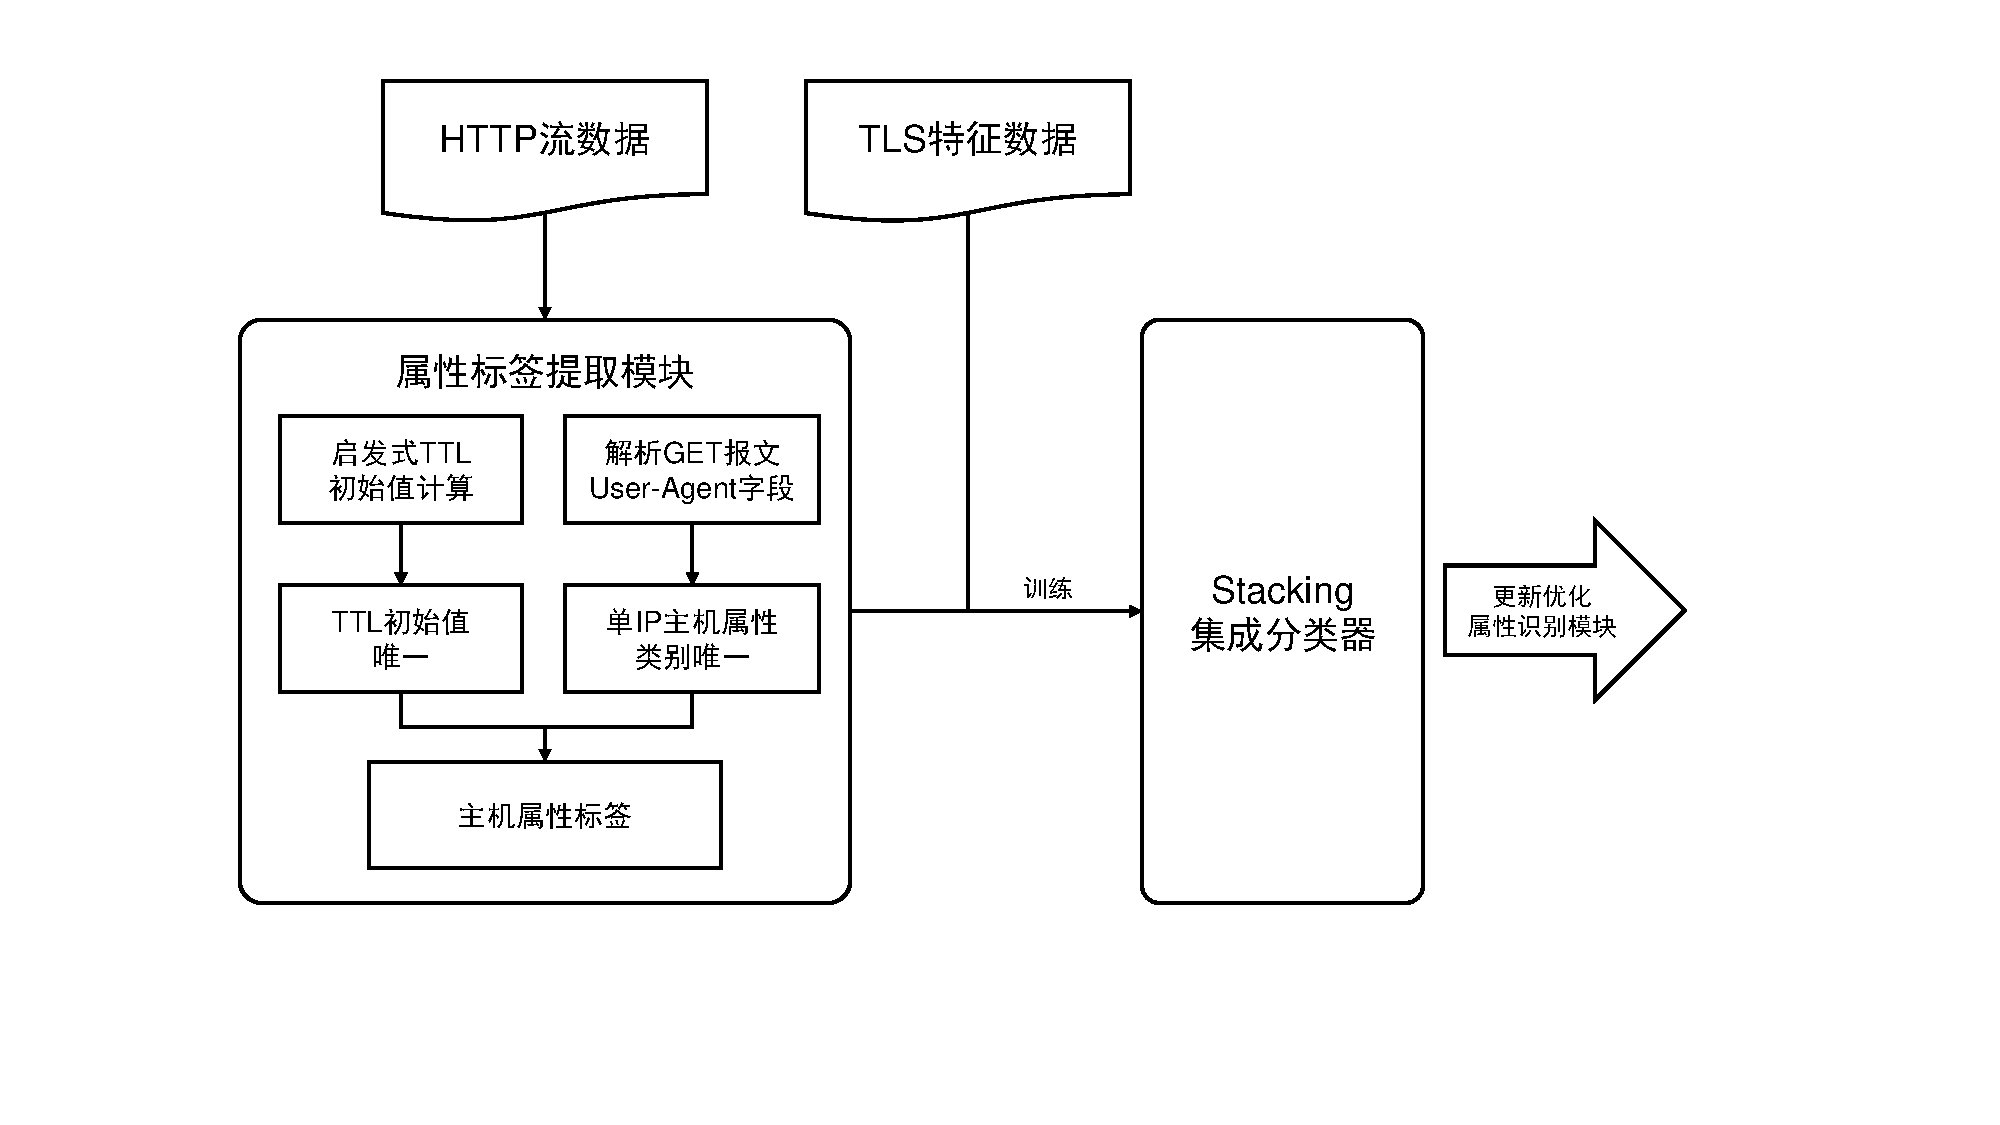
\includegraphics[width=0.9\textwidth]{5-4}
    \bicaption{分类器更新模块}{Classifier update module}
    \label{fig:5-4}
\end{figure}

由于考虑到系统的可扩展性,即在未来的主机属性发现场景中可能需要识别更多类别的操作系统和浏览器,分类器更新模块基于3.4节中介绍的属性标注方法,可以从HTTP流数据和TLS特征数据中构造有标签的数据集。然后分类器更新模块利用该数据集对Stacking集成模型进行离线训练,不会影响系统的实时识别功能。当离线模型的识别性能满足要求时,停止训练并将训练好的模型替换到属性识别模块中,完成对分类器的更新过程。

%由于本文中分类器的训练属于监督学习,必须基于有标签的数据集。而流量采集模块从网络中提取出的TLS流信息只包含训练任务所需的特征,并未携带主机属性标签。因此,本模块需要通过解析HTTP流GET请求报文中的User-Agent字段获取客户端的主机属性信息,然后通过客户端IP地址关联HTTP流与TLS流,为特征数据集完成属性标注。

%在当下的真实网络环境中,由于网络地址转换、动态主机配置协议等技术的存在,同一IP可能代理了多台局域网内的设备,导致在关联过程中,同一TLS流会被标注上不同的属性标签。如图5.7所示,三台不同类型的内网设备通过共享同一个公网地址即114.242.164.186访问因特网,对基于User-Agent字段的属性标注方法带来困难。为了解决这一问题,流量过滤模块利用同一客户端IP的主机属性应唯一、初始TTL值应唯一等假设筛选出单设备IP,通过此类IP的网络流量构建训练数据集。

\section{数据存储与可视化模块}

数据存储与可视化模块的功能主要是存储、查询与展示网络中已识别的主机属性信息。如图5.6所示,本模块首先利用Logstash工具从属性识别模块中收集三类主机属性的识别结果日志,从分类器更新模块中收集属性标注数据,并以Json格式存储到Elasticsearch数据库中。其中,识别结果日志的存储便于用户查询和数据分析,属性标注数据的存储用于将来分类器的模型更新和调整。然后时由ElasticSearch数据库携带的检索工具提供信息查询功能。最终借助Kibana工具生成展示给用户的Web界面,包括系统实时识别进度,网络中已检测主机的三类属性分布以及每天的吞吐量等。

\begin{figure}[!htbp]
    \centering
    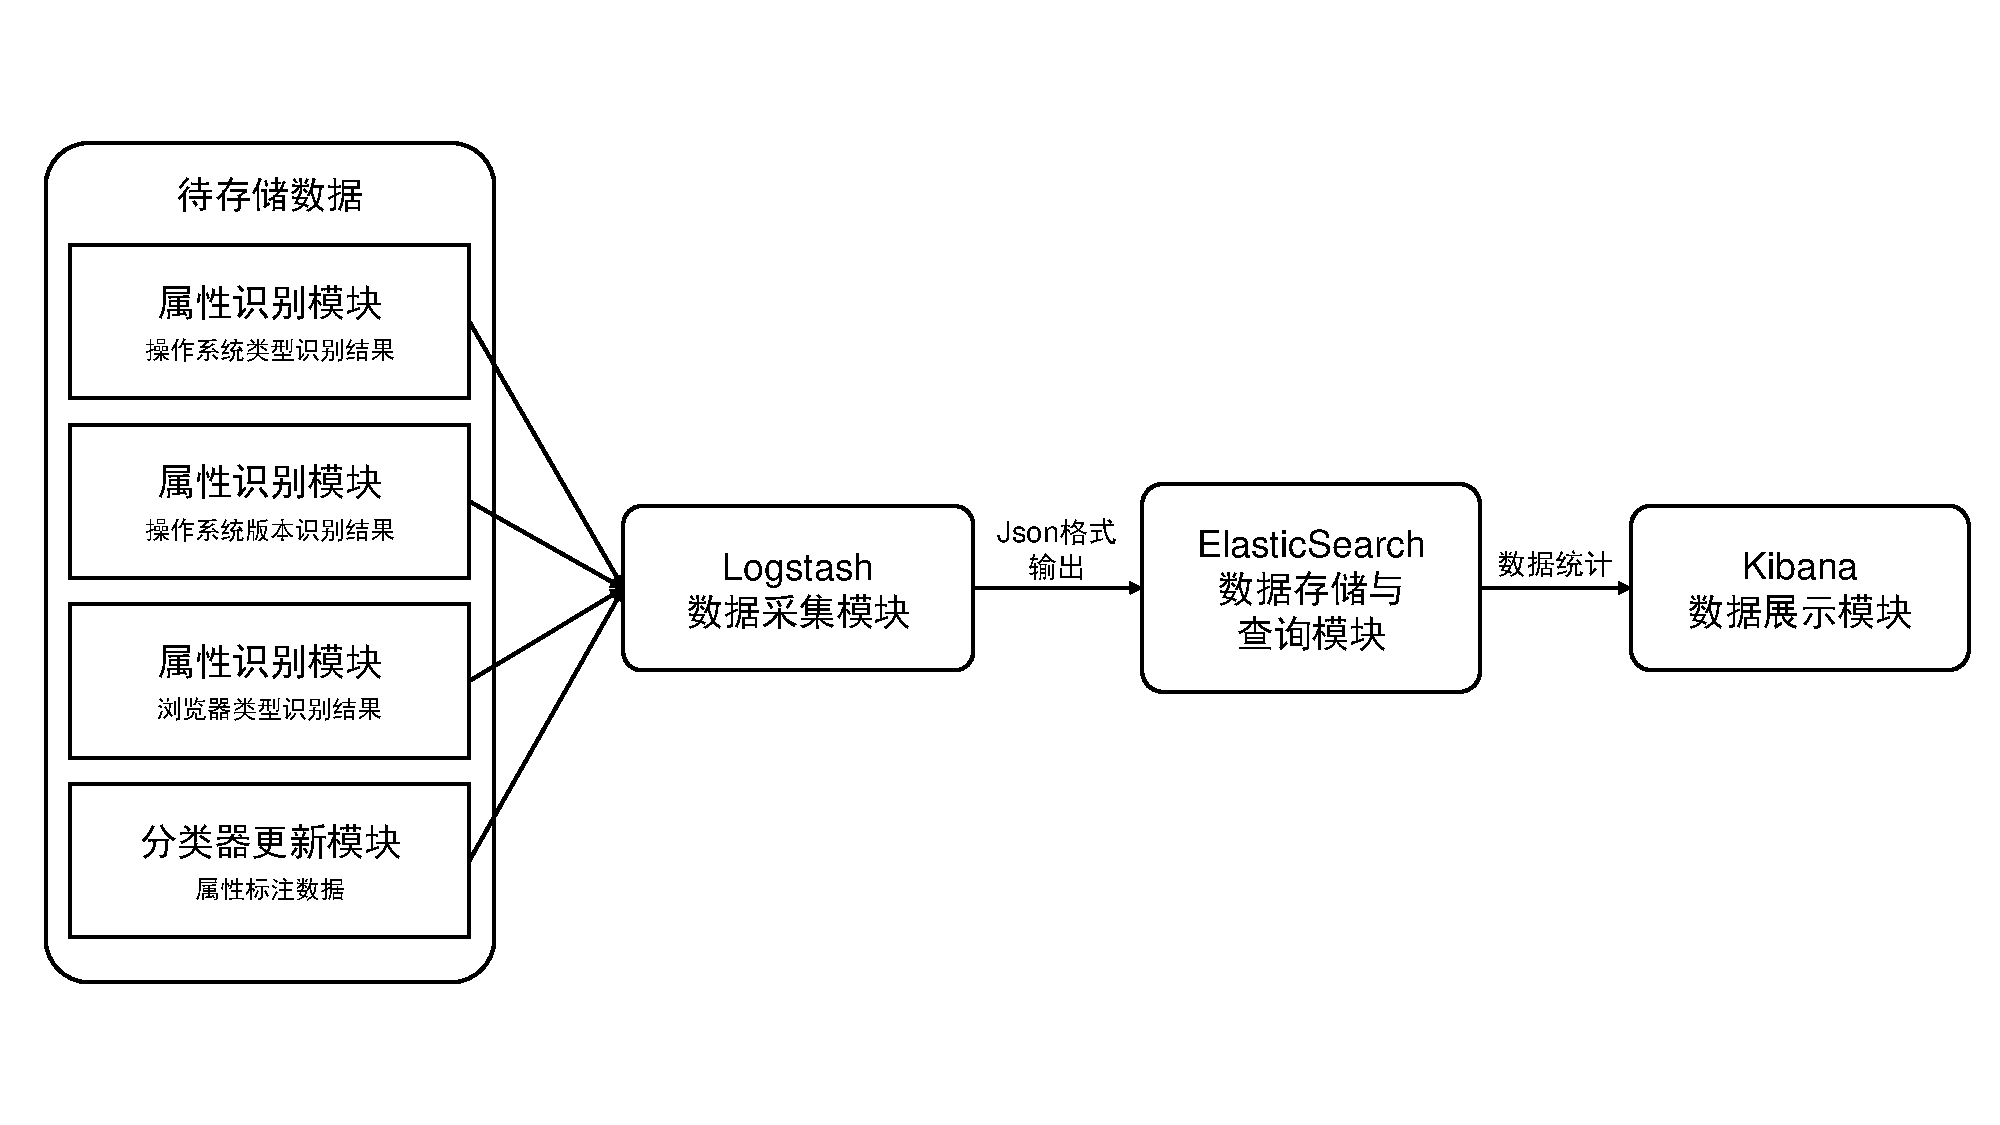
\includegraphics[width=0.9\textwidth]{数据存储}
    \bicaption{数据存储与可视化模块}{Data storage and visualization module}
\end{figure}

\section{系统测试}

\subsection{测试环境}

将本章介绍的原型系统实现后部署在某科研网络的实验环境中,环境配置如表5.1所示,操作系统为Ubuntu系统,CPU型号为Intel Xeon E5-2640,深度学习分类器采用的GPU型号为GTX 1080Ti,设备内存最大为94GB,网络中的流速均值为200MBps。在编程实现方面,流量采集模块与特征提取模块基于C语言实现,属性识别模块和分类器更新模块基于Python语言实现,数据存储和可视化模块基于ElasticSearch数据库实现。

\begin{table}[!h] 
    \bicaption{实验环境}{Lab environment}
    \centering
    \footnotesize
    \setlength{\tabcolsep}{25pt}
    \renewcommand{\arraystretch}{1}
\begin{tabular}{|c|l|}

\hline
操作系统 & Ubuntu 16.04.6 LTS \\ \hline
CPU型号 	& Intel Xeon E5-2640\\ \hline
GPU型号& GTX 1080Ti\\ \hline
内存大小& 94GB\\ \hline
网络流速 & 200MBps \\\hline

\end{tabular}
\end{table}

\subsection{系统运行性能测试}

本文在2020年1月3日到1月12日对系统进行为期十天的部署测试,观察并分析了系统在资源消耗方面和识别性能方面的表现,评估了原型系统在主机属性发现任务中的计算成本、空间成本以及识别有效性。

如表5.2所示,系统平均每天检测1465833条TLS会话,包含132075个客户端主机。在十天的运行结果中,对单核CPU的占用率峰值最高为87.4\%,内存率占用峰值最高为7.1\%,处理速度最快可以达到每分钟识别4357条会话。在GPU占用方面,基于Tensorflow实现的深度学习分类器对单核GPU的利用率最高可接近100\%。由此可见,本系统的计算复杂度较高,对内存空间的需求较小。在表5.1所示的实验条件下,系统可实现对主机属性的实时发现。

\begin{table}[!h] 
    \bicaption{系统运行性能}{System performance}
    \centering
    \footnotesize
    \setlength{\tabcolsep}{6pt}
    \renewcommand{\arraystretch}{1}
\begin{tabular}{ccccccc}
\toprule
天数 &TLS会话数目 &客户端主机数 & CPU峰值 & GPU峰值 & 内存峰值 & {\begin{tabular}[c]{@{}c@{}}吞吐量峰值\\ (样本/分钟)\end{tabular}}\\ 
\hline
1 & 1207243 & 135938  & 61.7\% & 98.8\% & 5.2\% & 3767\\
2 & 1649110 & 121809  & 87.4\% & 99.1\% &7.1\% &  4133\\
3 & 1601300 & 133736  & 76.9\% & 98.3\% &5.8\% &  3914\\
4 & 1371310 & 145284  & 50.2\% & 98.7\% &4.9\% &  3501\\
5 & 1689831 & 139410  & 51.3\% & 99.1\% &5.3\% &  3591\\
6 & 1494181 & 122342  & 67.6\% & 99.8\% &5.8\% &  3762\\
7 & 1282757 & 130111  & 81.4\% & 99.8\% &6.7\% &  4357\\
8 & 1589818 & 142170  & 70.3\% & 98.4\% & 6.1\% &  4206\\
9 & 1190328 & 122802  & 81.7\% & 99.7\% & 6.1\% &  3924\\
10 & 1582456 & 127149 & 81.2\% & 99.8\% & 6.3\% & 4008\\
均值 & 1465833 & 132075 &  70.9\% & 99.2\%& 5.9\% & 3916\\
\bottomrule
\end{tabular}
\end{table}

\subsection{分类器识别性能测试}

在系统测试过程中,本文发现,由于实时网络中的流量数据复杂多样,流量采集模块捕获的某些会话数据存在异常(缺失、噪声、不一致、冗余),无法提取有效特征,导致分类器不能有效识别其主机属性信息。

此外,由于属性识别模块目前的识别范围是有限的,只能识别主流的操作系统类型、版本以及浏览器类型。而在开放的实验网络中,可能存在识别范围之外的TLS会话数据,例如Symbian系统、BlackBerry OS系统、360浏览器、QQ浏览器等操作系统或浏览器发起的TLS会话。这些会话样本数据虽然占比非常小,但可能在一定程度上导致分类器的误识别,降低识别准确性。

为了筛选出上述问题产生的异常会话样本,本文优化了分类器的识别策略。在一般的分类器识别过程中,机器学习模型会对每个样本预测其属于某个类别的概率,然后选择概率最大的类别作为识别结果。通过深入统计分析,我们发现分类器对异常样本的类别预测概率通常都低于50\%。因此,本文假设仅当分类器的类别预测概率最大值高于50\%时,才会选择概率最大的类别作为识别结果,否则视为识别失败,即该样本不属于任何类别。

\begin{table}[!h] 
    \bicaption{分类器识别性能}{Classifier identification performance}
    \centering
    \footnotesize
    \renewcommand{\arraystretch}{1}
\begin{tabular}{ccccccc}
\toprule
\multirow{2}{*}{天数} & \multicolumn{3}{c}{识别率} & \multicolumn{3}{c}{F1分数} \\ \cline{2-7}
& 操作系统类型 & 操作系统版本 & 浏览器类型 &操作系统类型 & 操作系统版本 & 浏览器类型 \\ \hline
1 & 95.11\% & 94.13\% & 91.61\% & 96.51\% & 79.92\% & 95.14\% \\
2 & 94.25\% & 93.71\% &  91.53\% & 95.16\% & 82.79\% & 94.87\% \\
3 & 95.24\% & 94.11\% & 91.60\% & 96.47\% & 82.82\% & 94.98\% \\
4 & 93.71\% & 91.93\% & 92.33\% & 96.23\% & 82.83\% & 95.25\% \\
5 & 95.92\% & 94.27\% & 89.96\% & 96.01\% & 80.78\% & 95.54\% \\
6 & 96.30\% & 93.67\% & 92.41\% & 96.53\% & 81.13\% & 95.51\% \\
7 & 96.11\% & 95.86\% & 93.40\% & 95.90\% & 80.72\% & 96.20\% \\
8 & 91.62\% & 91.07\% & 92.42\% & 96.22\% & 82.09\% & 94.74\% \\
9 & 95.98\% & 93.24\% & 92.99\% & 96.48\% & 79.72\% & 96.22\% \\
10 & 94.42\% & 93.19\% & 91.94\% & 96.21\% & 81.14\% & 95.85\% \\
均值& 94.87\% & 93.52 \% & 92.02\%  & 96.17\% & 81.40\% & 95.43\% \\
\bottomrule
\end{tabular}
\end{table}

在如表5.3所示的分类器识别性能测试结果中,系统对操作系统类型的识别成功率均值为94.87\%,对操作系统版本的识别成功率均值为93.52\%,对浏览器类型的识别成功率均值为92.02\%。其中,系统对浏览器类型识别的成功率最低,这主要是因为实验网络中较多主机使用了识别范围之外的小众浏览器。

F1分数是模型精确度的一种指标。它同时兼顾了分类模型的精确率和召回率。从表5.3所示分类结果的F1分数来看,属性识别模块中的Stacking集成模型比第3章和第4章中介绍的所有单一模型效果都要更好,充分体现了Stacking技术的优越性。此外,系统在十天中的各方面性能变化都比较小,最大差异没有超过3\%,这一结果也证明了本系统拥有较强的稳定性和鲁棒性。

\subsection{可视化功能测试}

本文在2020年1月12日晚截取了系统的实时可视化Web页面,如图5.7所示,主要向用户展示了系统当日已识别的客户端数目,每天处理的会话数目以及各种主机属性的统计结果等。除此之外,系统还可以根据需要从数据库中快速检索并绘制更多表格和图像,方便用户对识别结果进行观察和分析。

\begin{figure}[!htbp]
    \centering
    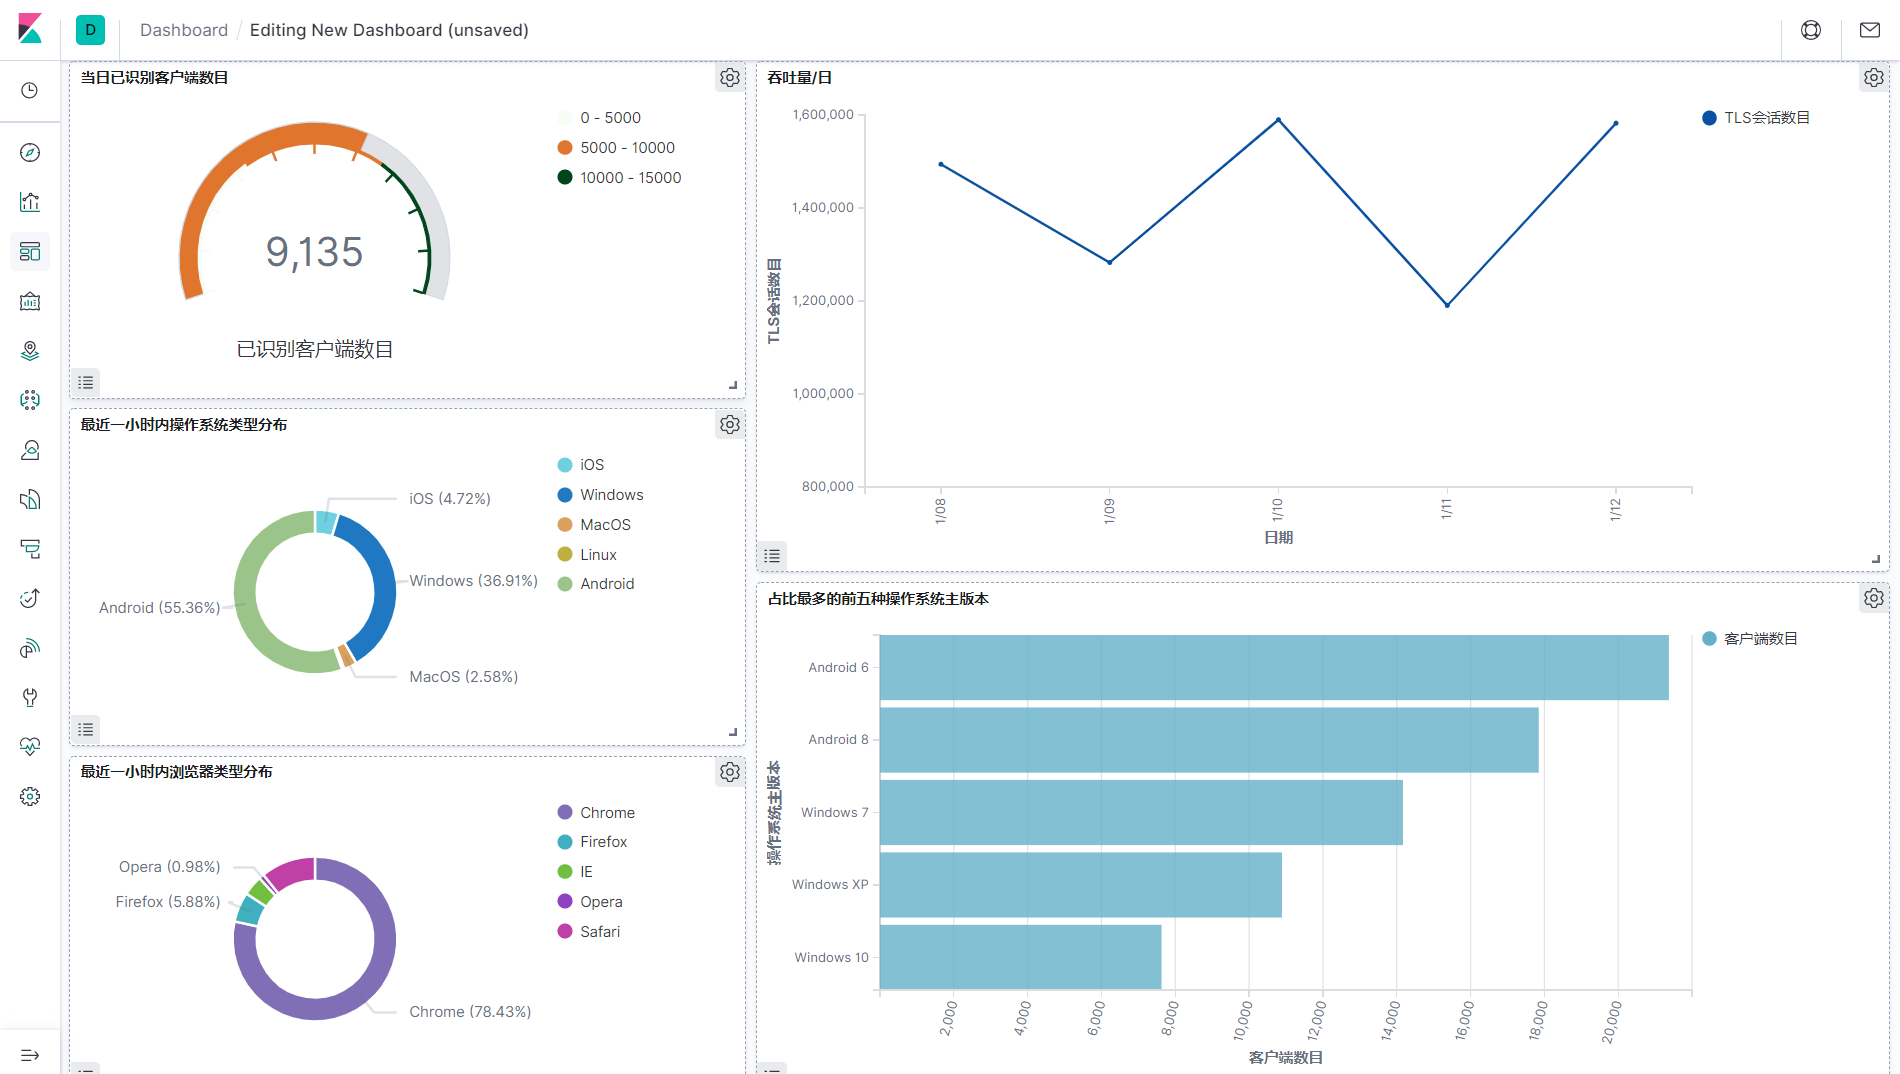
\includegraphics[width=0.8\textwidth]{可视化}
    \bicaption{可视化页面}{Visual page}
\end{figure}

\subsection{识别结果分析}

在为期十天的系统测试结果中,本系统共发现了5种操作系统类型,5种浏览器类型和22种操作系统版本,操作系统类型主要为Android、Windows、iOS、MacOS以及Linux等,版本包括上述5种操作系统的22种主版本,浏览器类型主要为Chrome、Safari、IE、Firefox以及Opera等。

在图5.8所示的操作系统类型识别结果中,Android系统和Windows系统的数量最多,共计占比约87.3\%,其次是Apple公司设计开发的iOS系统和MacOS系统,约占10\%,Linux系统的数量最少,只有2.7\%。

\begin{figure}[!h]
    \centering
    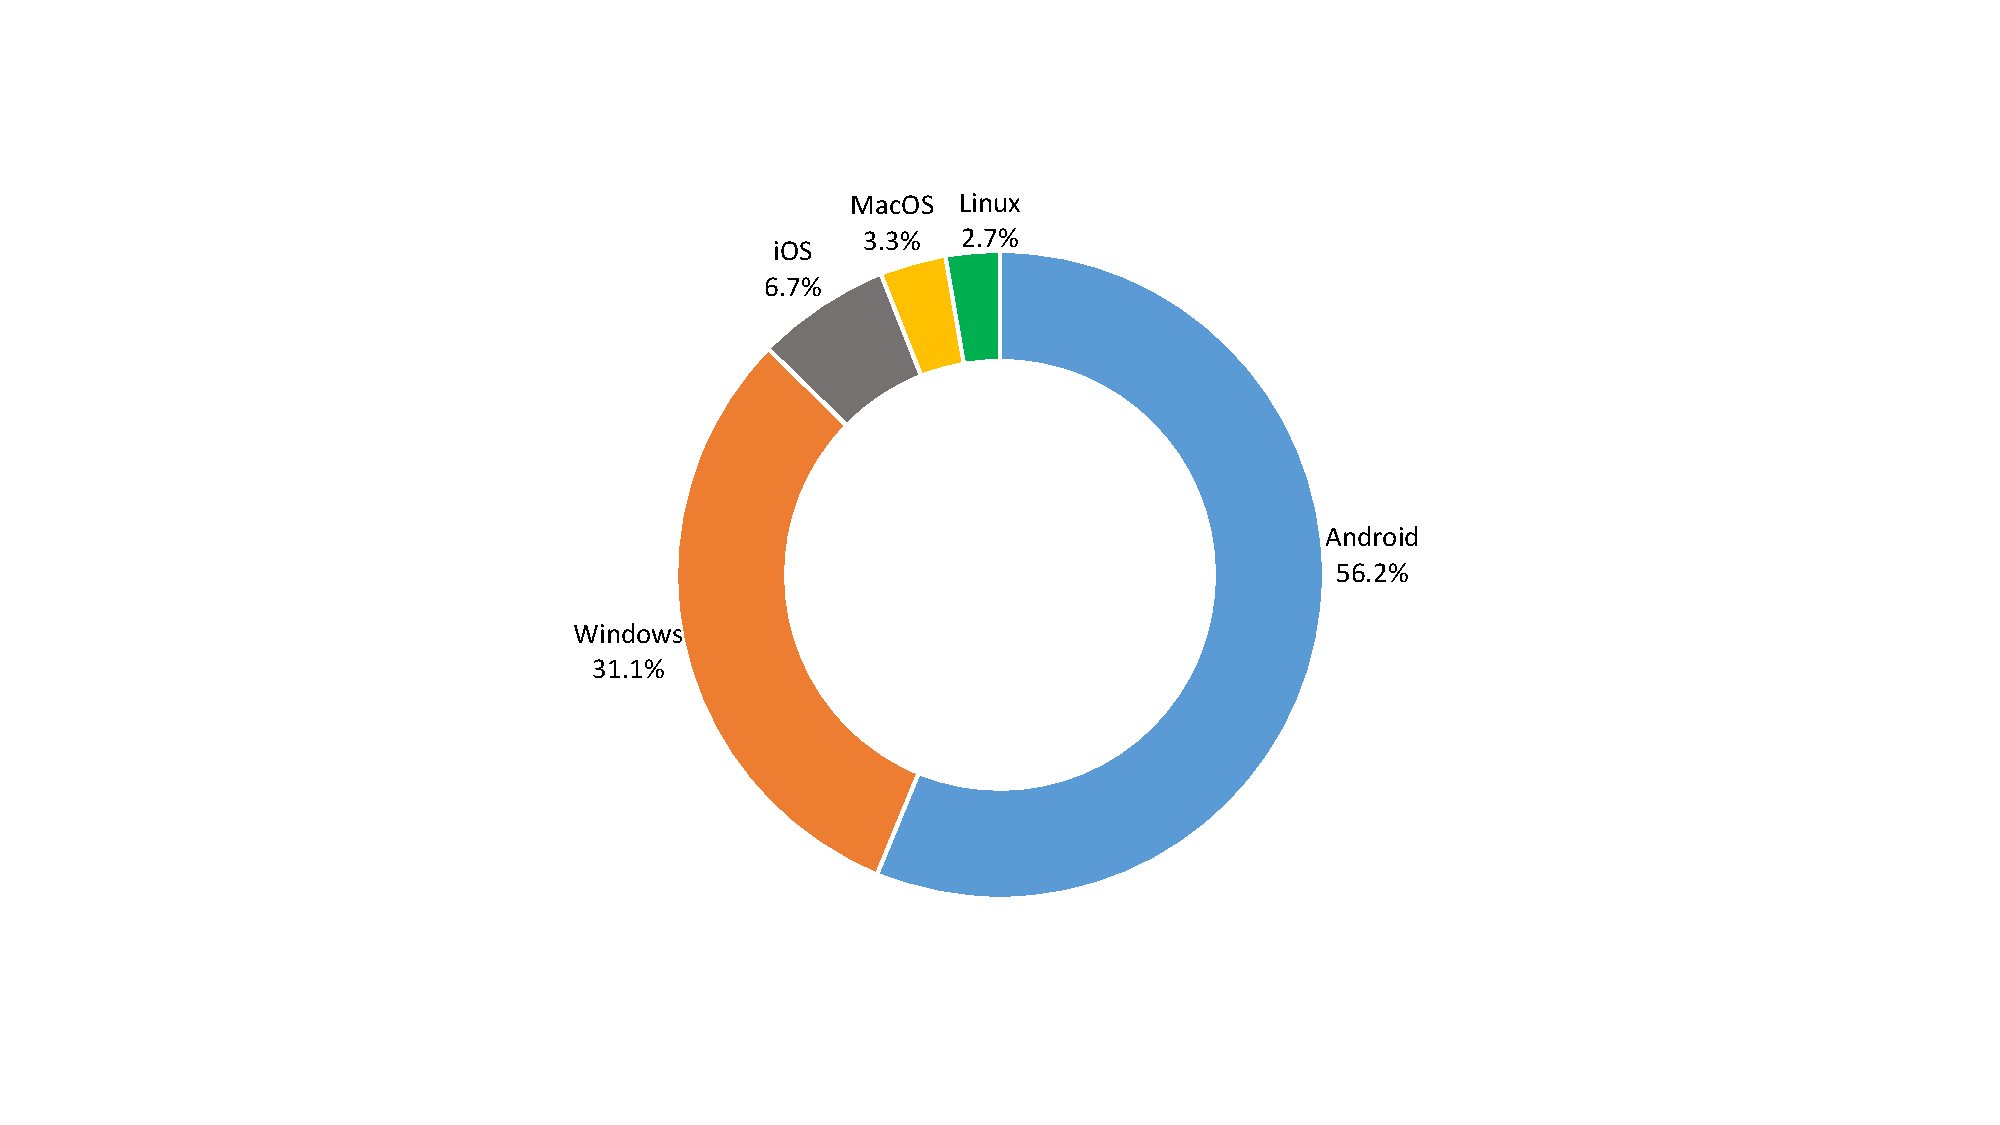
\includegraphics[width=0.59\textwidth]{os类型分布}
    \bicaption{识别结果中的操作系统类型分布}{Distribution of operating system type  in the identify ressults}
\end{figure}

在浏览器类型识别结果中,如图5.9所示,最受用户欢迎的浏览器是Chrome浏览器,占比约为70.6\%,比排名第二的Safari浏览器多出近50\%。IE浏览器作为微软公司的官方浏览器和Windows系统的默认浏览器,其使用量却非常少,仅占比约4.9\%。而经典的Firefox浏览器和Opera浏览器则更为少见,共计占比约4.8\%。

\begin{figure}[!h]
    \centering
    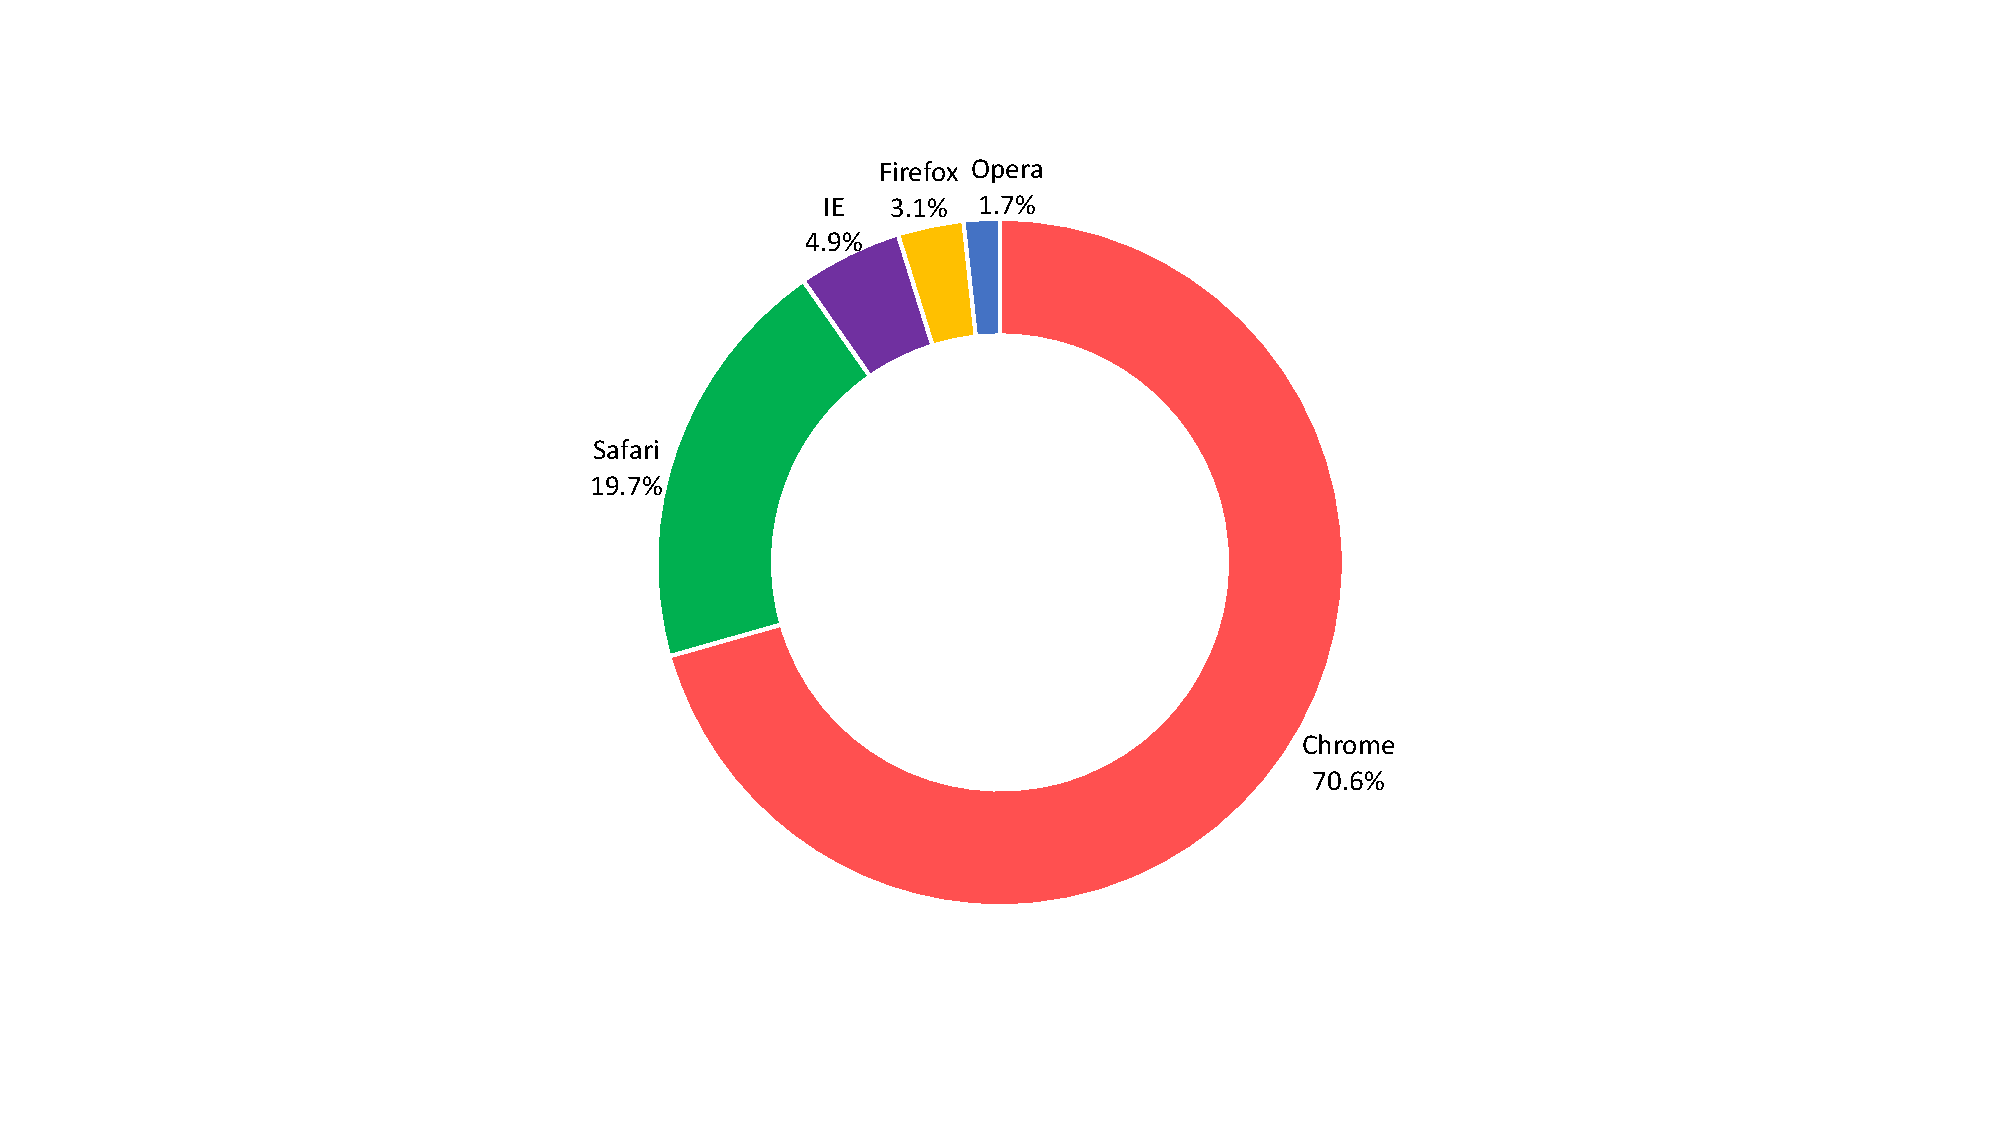
\includegraphics[width=0.55\textwidth]{bs类型分布}
    \bicaption{识别结果中的浏览器类型分布}{Distribution of browser type in the identify ressults}
\end{figure}

图5.10展示了操作系统版本的识别结果分布,从中可以发现,无论是最常见的Android系统和Windows系统,还是较为小众的iOS系统和MacOS系统,在其历史版本中,使用量最多的往往不是最新版本,而是稳定性和兼容性较好的经典版本。此外,在所有版本的系统中,Android 6、Android 8以及Windows 7系统的占比最多,共为49.5\%,
\begin{figure}[!h]
    \centering
    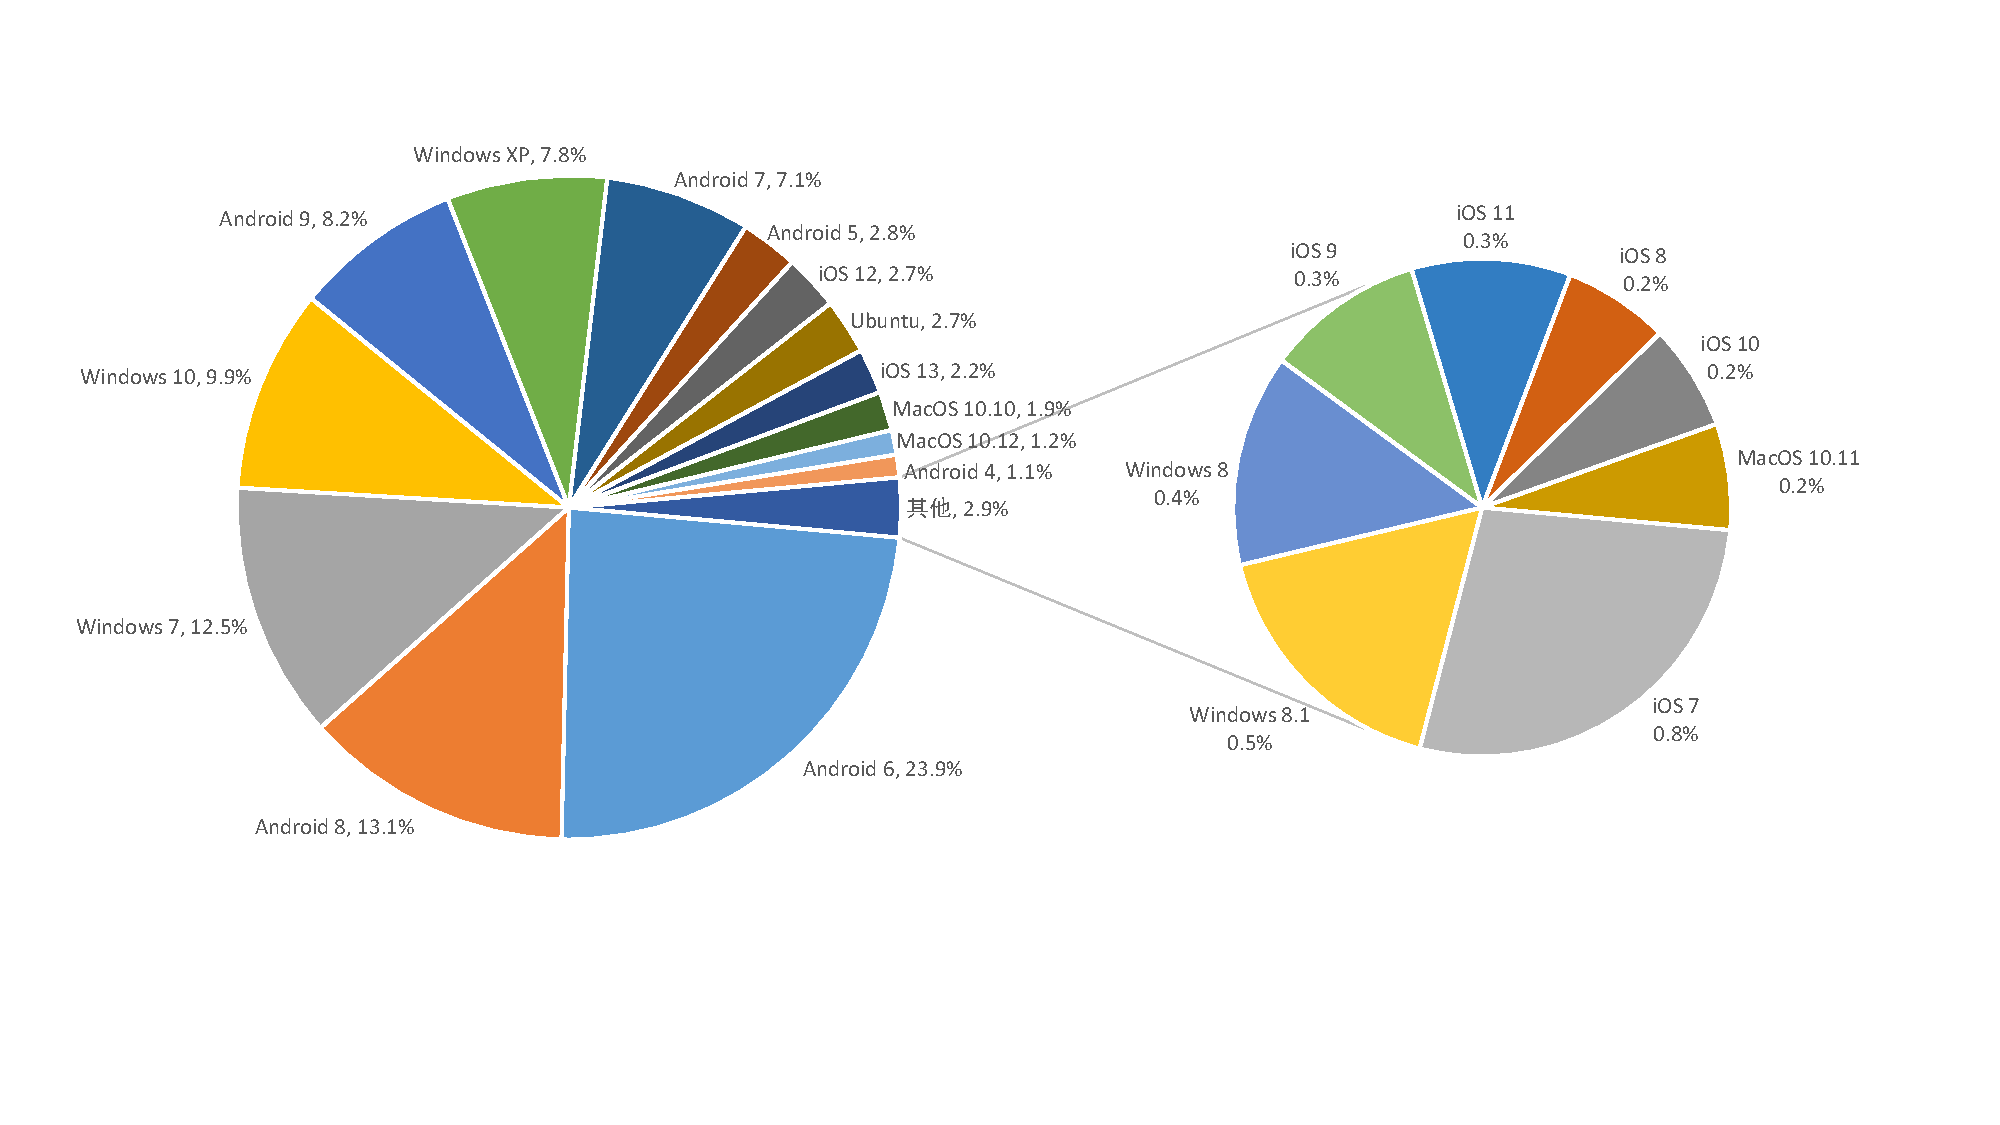
\includegraphics[width=0.9\textwidth]{os版本分布}
    \bicaption{操作系统版本分布}{Operating system Version distribution}
\end{figure}

\section{本章小结}

本章基于前文的研究成果,设计并实现了一个基于加密流量指纹的主机属性发现原型系统。本系统首先从实时网络中识别和采集HTTP流量和TLS流量,以五元组为标识将每个网络会话的所有数据包按序汇集为双向流。然后从流中提取所需特征和标签,特征主要包括协议首部字段特征、流统计特征以及流原始字节特征,标签主要为从HTTP协议首部User-Agent字段中提取出的主机属性信息。根据特征数据,系统中的Stacking集成分类器可快速、准确地识别每条TLS流的主机属性信息,同时结合标签数据,系统可完成对分类器的更新与优化。最终,基于Elasticsearch开源搜索平台,实现对识别信息的存储、查询与可视化。

通过在实时网络中部署并进行为期十天的测试,完成了对原型系统的性能评估,证明了系统具有优秀的鲁棒性和识别精度,其提供的可视化功能可以方便用户观察识别结果。

\chapter{总结与展望}
随着网络攻击行为日趋复杂,政府、企业以及个人所面临的安全威胁正在飞速增长,如蠕虫病毒、木马后门、僵尸网络、DDOS攻击等,给企业的信息网络造成严重破坏。保障网络安全最大的挑战之一就是及时发现漏洞,而绝大部分安全漏洞和隐患都与主机属性息息相关。此外,识别网络中主机的多维属性还可以帮助网络运营者有效地进行网络管理、网络资源分配、网络服务质量优化。

\section{本文工作总结}

本文主要完成了以下三点工作:

\begin{enumerate}
    \item \textbf{开放环境中的细粒度主机属性发现。}首先以流为单位,提取目标主机发起的TLS会话中的13维协议首部字段特征和3类流统计特征,包括IP协议的跳数、包长、分片标识等字段,TCP协议的传输窗口大小、窗口缩放因子、最大报文长度等字段,TLS协议的版本、扩展长度、密钥算法套件序列等字段以及流的包长序列统计特征、时间序列统计特征、速率统计特征等。然后结合以LightGBM模型为代表的机器学习算法,识别目标主机的操作系统类型及版本、浏览器类型及版本。
    
    \item \textbf{基于加密流原始载荷的主机属性发现。}随着理论的成熟和机器性能的提升,深度学习模型在流量分类领域里的表现越来越出色。通过提取TLS会话中TCP握手包和Client-Hello包的原始流信息,并结合以CNN模型和LSTM模型为代表的表示学习算法,便可在不需要先验知识的前提下,进一步提高复杂网路中主机属性的识别精度。
    
    \item \textbf{大规模网络中的海量主机属性发现。}本文基于Stacking技术,结合以人工特征为基础的LightGBM模型和以原始流信息为基础的深度学习模型,构建了一个用于海量主机属性发现的原型系统。该系统主要包含四个模块。协议识别模块用于在高速网络中检测、解析并识别TLS流量。特征提取模块用于从原始TLS流量中提取所需的人工特征和原始特征。属性识别模块基于stacking技术,综合各学习模型的的检测结果,得到最终的识别信息。数据存储和可视化模块用于识别结果的存储和可视化展示。
\end{enumerate}

\section{下一步的工作}

本文对加密网络中的主机属性发现技术进行了深入分析,利用协议首部字段特征、流统计特征以及原始字节特征,结合统计机器学习模型和神经网络模型,实现了一套具备良好效果的原型系统,但仍然存在以下问题:

\textbf{构建更可信的标注数据集。}本文利用HTTP协议请求报文的User-Agent字段对数据集进行属性标注,标注的正确性依赖于User-Agent字段的真实性。而User-Agent字段容易篡改和伪装,可能一定程度上影响了属性标注方法的准确性,降低了分类器的识别性能。未来将尝试利用TLS透明代理技术或者与大型网络服务商合作,构建更真实可信的标注数据集。

\textbf{提高系统性能。}由于机器学习模型算法效率受限,本文方法的计算成本较高。今后需要从特征和模型角度入手,优化特征集规模,降低机器学习模型复杂度,提高识别效率。

\textbf{扩展主机属性种类。}本文系统目前仅能识别三类主机属性,包括操作系统种类、版本以及浏览器种类等。识别的类别数目较少,未来工作可以引入更多的主机属性,例如设备类型、设备厂商、主机地理位置等等。

\textbf{分析新型协议。}本文的研究对象主要是采用加密协议TLS 1.2版本或更早版本的网络会话,在未来各种新型协议如QUIC协议、TLS 1.3协议、HTTP 2.0协议等技术的普及将会给主机属性识别带来新的挑战。
%---------------------------------------------------------------------------%
% main content
%-
%-> Appendix
%-
\cleardoublepage%
\appendix% initialize the environment
%\chapter{中国科学院大学学位论文撰写要求}

学位论文是研究生科研工作成果的集中体现,是评判学位申请者学术水平、授予其学位的主要依据,是科研领域重要的文献资料。根据《科学技术报告、学位论文和学术论文的编写格式》(GB/T 7713-1987)、《学位论文编写规则》(GB/T 7713.1-2006)和《文后参考文献著录规则》(GB7714—87)等国家有关标准,结合中国科学院大学(以下简称“国科大”)的实际情况,特制订本规定。

\section{论文无附录者无需附录部分}

\section{测试公式编号 \texorpdfstring{$\Lambda,\lambda,\theta,\bar{\Lambda},\sqrt{S_{NN}}$}{$\textLambda,\textlambda,\texttheta,\bar{\textLambda},\sqrt{S_{NN}}$}} \label{sec:testmath}

\begin{equation} \label{eq:appedns}
    \adddotsbeforeeqnnum%
    \begin{cases}
        \frac{\partial \rho}{\partial t} + \nabla\cdot(\rho\Vector{V}) = 0\\
        \frac{\partial (\rho\Vector{V})}{\partial t} + \nabla\cdot(\rho\Vector{V}\Vector{V}) = \nabla\cdot\Tensor{\sigma}\\
        \frac{\partial (\rho E)}{\partial t} + \nabla\cdot(\rho E\Vector{V}) = \nabla\cdot(k\nabla T) + \nabla\cdot(\Tensor{\sigma}\cdot\Vector{V})
    \end{cases}
\end{equation}
\begin{equation}
    \adddotsbeforeeqnnum%
    \frac{\partial }{\partial t}\int\limits_{\Omega} u \, \mathrm{d}\Omega + \int\limits_{S} \unitVector{n}\cdot(u\Vector{V}) \, \mathrm{d}S = \dot{\phi}
\end{equation}
\[
    \begin{split}
        \mathcal{L} \{f\}(s) &= \int _{0^{-}}^{\infty} f(t) e^{-st} \, \mathrm{d}t, \ 
        \mathscr{L} \{f\}(s) = \int _{0^{-}}^{\infty} f(t) e^{-st} \, \mathrm{d}t\\
        \mathcal{F} {\bigl (} f(x+x_{0}) {\bigr )} &= \mathcal{F} {\bigl (} f(x) {\bigr )} e^{2\pi i\xi x_{0}}, \ 
        \mathscr{F} {\bigl (} f(x+x_{0}) {\bigr )} = \mathscr{F} {\bigl (} f(x) {\bigr )} e^{2\pi i\xi x_{0}}
    \end{split}
\]

mathtext: $A,F,L,2,3,5,\sigma$, mathnormal: $A,F,L,2,3,5,\sigma$, mathrm: $\mathrm{A,F,L,2,3,5,\sigma}$.

mathbf: $\mathbf{A,F,L,2,3,5,\sigma}$, mathit: $\mathit{A,F,L,2,3,5,\sigma}$, mathsf: $\mathsf{A,F,L,2,3,5,\sigma}$.

mathtt: $\mathtt{A,F,L,2,3,5,\sigma}$, mathfrak: $\mathfrak{A,F,L,2,3,5,\sigma}$, mathbb: $\mathbb{A,F,L,2,3,5,\sigma}$.

mathcal: $\mathcal{A,F,L,2,3,5,\sigma}$, mathscr: $\mathscr{A,F,L,2,3,5,\sigma}$, boldsymbol: $\boldsymbol{A,F,L,2,3,5,\sigma}$.

vector: $\Vector{\sigma, T, a, F, n}$, unitvector: $\unitVector{\sigma, T, a, F, n}$

matrix: $\Matrix{\sigma, T, a, F, n}$, unitmatrix: $\unitMatrix{\sigma, T, a, F, n}$

tensor: $\Tensor{\sigma, T, a, F, n}$, unittensor: $\unitTensor{\sigma, T, a, F, n}$ 


% appendix content
%-
%-> Backmatter: bibliography, glossary, index
%-
\backmatter% initialize the environment
\intotoc*{\cleardoublepage}{\bibname}% add link to toc
%\nocite{*}
\bibliography{Biblio/ref}% bibliography
%---------------------------------------------------------------------------%
%->> Backmatter
%---------------------------------------------------------------------------%

\chapter[致谢]{致\quad 谢}\chaptermark{致\quad 谢}% syntax: \chapter[目录]{标题}\chaptermark{页眉}
\thispagestyle{noheaderstyle}% 如果需要移除当前页的页眉
%\pagestyle{noheaderstyle}% 如果需要移除整章的页眉

时光荏苒,岁月如梭,转眼间三年的硕士生涯即将结束。在毕业设计完成之际,我要衷心地感谢给予我无私帮助的老师,同学和家人。

感谢我的导师周晓飞老师。周老师学问扎实、工作严谨,三年间在生活和学习中给予了我很多的帮助。感谢熊刚老师,熊老师工作兢兢业业,锐意进取,认真踏实,是我们整个课题组学习的榜样,更是我人生道路上的导师。感谢给予我学术指导的苟高鹏老师和康翠翠老师,研究生期间的学术成果离不开两位老师的帮助。苟老师在学术研究上对自身有很高的要求,在科研方面给我提供了很多宝贵的意见。感谢石俊峥老师,石老师工作兢兢业业,认真踏实,在工程实践方面的丰富经验和严谨态度对我造成了非常积极的影响。

感谢实验室同窗们的陪伴和帮助。感谢崔明鑫师兄,侯承尚师兄,张龙师兄,刘晓龙师兄,刘畅师姐,郭煜师姐,杨颖师姐在学术和生活中对我的鼓励和指导。感谢王宇同学,王海同学,吴悠漾同学,王思源同学。三年间,我们一起学习工作,一起生活娱乐,一起守望互助,一起憧憬未来。感谢李思佳同学,让我收获研究生期间最大的惊喜。

感谢我的父母和姐姐。感谢父母的养育之恩,感谢家人作为我的精神支柱,激励着我在人生道路上不断前行。

最后,再次衷心感谢所有帮助我、关心我、支持我的老师、同学和亲友。

\chapter{作者简历及攻读学位期间发表的学术论文与研究成果}

\section*{作者简历}

范鑫磊,山东省菏泽市人,中国科学院信息工程研究所硕士研究生。


\section*{已发表(或正式接受)的学术论文:}

Identify OS from encrypted traffic with TCP/IP stack fingerprinting, IPCCC 2019.

\section*{申请或已获得的专利:}

一种基于TCP/IP协议栈指纹的操作系统被动识别方法

\section*{参加的研究项目及获奖情况:}

协议解析示范应用

特定app流量数据包分析课题

2018-2019学年中国科学院大学三好学生

%\cleardoublepage[plain]% 让文档总是结束于偶数页,可根据需要设定页眉页脚样式,如 [noheaderstyle]
%---------------------------------------------------------------------------%
% other information
\end{document}
%---------------------------------------------------------------------------%

